\section*{Úvod}



Soubor obsahuje příklady pro cvičení k mým přednáškám na Lesnické a dřevařské fakultě pro bakalářské studium v letním semestru 2020. Text bude expandovat, jak poběží semestr. Vychází ze cvičení v minulém semestru (kompletní zadání a většina řešení jsou k dispozici na webu předmětu). Text existuje ve verzích pro tisk na papír a pro promítání na plátně, každá z těchto verzí ještě s řešeními a bez řešení. 

\stranka
\section{Výpočet derivací}

Derivaci budeme chápat jako zobrazení, které funkci přiřadí jinou
funkci. Proč je tak nesmírně užitečná zjistíme v následujících
týdnech.

\def\tg{\mathop{\mathrm{tg}}}
\def\cotg{\mathop{\mathrm{cotg}}}
\def\arctg{\mathop{\mathrm{arctg}}}

\def\derivace#1;#2\par{$\displaystyle{(#1)'=\frac{\mathrm d}{\mathrm dx}(#1)=#2}$\par\smallskip}

\textbf{Základní vzorce.}

\bigskip
\hbox to \hsize{\begin{minipage}[t]{0.5\linewidth}
\derivace c;0

\derivace x^n;n x^{n-1}

\derivace e^x;e^x

\derivace \ln x;\frac 1x

\end{minipage}
\begin{minipage}[t]{0.5\linewidth}
\derivace \sin x;\cos x

\derivace \cos x;-\sin x

\derivace \arctg x;\frac 1{1+x^2}

\end{minipage}} Zde $c\in\mathbb R$ je konstanta a zbytek jsou vzorce,
které platí vždy, když je výraz napravo definovaný.

\stranka 

\textbf{Triky, které se často hodí.}
\begin{multicols}3
\begin{enumerate}[(A)]
\item $\sqrt x=x^{\frac 12}$
\item 
$\sqrt[k] x=x^{\frac 1k}$
\item 
$\frac {1}{x^k}=x^{-k}$
\item 
$\frac {f(x)}c=\frac 1c f(x)$
\item 
$\frac {c}{f(x)}=c f^{-1}(x)$
\item 
$a^x=e^{x\ln a}$
\item 
$\log_ax=\frac{\ln x}{\ln a}$
\item $\sqrt x(x+1)=x^{\frac 32}+x^{\frac 12}$
\item $\frac  {x^3+4}{x^2}=x+4x^{-2}$
\end{enumerate}

\end{multicols}

\stranka 
\textbf{Derivování a operace mezi funkcemi}

  Nechť $f$, $g$ jsou funkce a $c\in\mathbb R$ konstanta. Platí
  \begin{align*} 
    {\left[cf\right]}'&=cf',\\
    {\left[f\pm g\right]}'&=f'\pm g',\\
    {\left[fg\right]}'&=f'g+fg',\\
    {\Bigl[\frac{f}{g}\Bigr]}'&=\frac{f'g-g'f}{g^2},\\
    \bigl[f(g(x))\bigr]'&=\frac{\mathrm df}{\mathrm dg}\frac{\mathrm dg}{\mathrm dx}=f'(g(x))g'(x)
  \end{align*}

  \stranka 
  \def\der #1.{$\vphantom{\frac 11}f(x)=#1$}
\subsection{Výpočet derivace}
Určete derivace následujících funkcí, kde $a,b,\mu\in\mathbb{R}$.
\begin{multicols}3
\begin{enumerate}
\item \der x^6+\frac 1{x^6}.
\item \der x^2+2x+6.
\item $f(r)=r^3+2r^2-1$
\item \der 3x\sqrt x+9x^5.
\item \der 1-e^{bx}.
\item \der (x^2-1)^4.
\item \der \frac{1}{\sqrt \pi}e^{ax^2}.
\item \der \frac 1{(x+6)^2}.
\item   \der \frac{a}{(\mu x+b)^2}.
\end{enumerate}
\end{multicols}

\def\der#1.{$f'(x)=#1$}
\reseni
\begin{multicols}2
  \begin{enumerate}
  \item \der 6x^5-\frac{6}{x^7}.
  \item \der 2x+2.
  \item $f'(r)=3r^2+4r$
  \item \der (3x^{3/2}+9x^5)'=\frac 92\sqrt x+45x^4.
  \item \der -be^{bx}.
  \item \der 4(x^2-1)^32x=8x(x^2-1)^3.
  \item \der \frac 1{\sqrt \pi} e^{ax^2}2ax.
  \item \der \frac{-2}{(x+6)^3}.
  \item \der \frac{-2a\mu}{(\mu x+b)^3}.
  \end{enumerate}
\end{multicols}
\konec

\def\jednotka #1#2{\left[\frac{\mathrm{d}#1}{\mathrm{d}#2}\right]}
\def\derivace #1#2{\frac{\mathrm{d}#1}{\mathrm{d}#2}}


\stranka
\obrazek[wikimedia.org]{ryba.jpg}
\subsection{Růst ryby}
Biologové navrhli funkci
  \begin{equation*}
    l=0.03937 t^3 - 0.945 t^2 + 10.033 t + 3.073
  \end{equation*}
  jako model délky jistého druhu ryby, kde $l$ je délka ryby v~centimetrech, a $t$ je věk v~letech.  Vypočtěte derivaci
  $\frac{\mathrm{d}l}{\mathrm {d}t}$. Určete jednotku této derivace a
  slovní interpretaci hodnoty derivace v~bodě $t=12$.

\textit{Upraveno podle Stewart, Day: Biocalculus. Calculus for the life siences. V tomto příkladě se setkáváme s klasickou interpretací derivace jako rychlosti změny, tj. hodnoty o kterou se změní závislá veličina, když se nezávislá veličina změní o jednotku.}

\reseni $\jednotka lt=\mathrm{cm}/\mathrm{rok}$, tj. centimetr za rok. Platí
  \begin{equation*}
    \derivace lt =3\cdot 0.03937 t^2 - 2\cdot 0.945 t + 10.033 =
    0.11811 t^2 -1.89 t + 10.033 
  \end{equation*}
  a pro $t=12\,\mathrm{let}$ dostáváme 
  \begin{equation*}
   \derivace lt\Bigr\vert_{t=12} =4.4\, \mathrm{cm}/\mathrm{rok}.
  \end{equation*}
  Dvanáctiletá ryba roste rychlostí přibližně $4.4$ centimetrů za rok,
tj. mezi dvanáctým a třináctým rokem vyroste přibližně o $4.4$
centimetru.

\konec


\stranka

\obrazek{kolibrik.jpg}
\subsection{Bazální metabolismus}
Bazální metabolismus $M$ (ve wattech) souvisí s hmotností $W$ vztahem
$$M=AW^n,$$ kde $n$ je pro mnoho živočišných druhů blízké číslu $0.75$ a
$A$ je konstanta, která je specifická pro daný druh a v rámci daného
druhu klesá s věkem. Určete derivaci $$\frac{\mathrm d M}{\mathrm dW}$$
a určete i fyzikální jednotku a slovní interpretaci této derivace.

\textit{Zpracováno podle Monteith, Unsworth: Principles of Environmental Physics. Tady je opět klasická interpretace derivace jako rychlosti změny. Rychlost změny ale nemusí být jenom klasické chápání rychlosti jako závislosti na čase. Derivace vyjadřuje, jak závislá veličina reaguje na změny nezávislé veličiny. Pro pochopení, co derivace vyjadřuje, hraje velkou roli i jednotka této derivace. Označení je ponecháno z původní literatury, mimo jiné $M$ není hmotnost a $W$ není watt. Vztah je v literatuře znám jako Kleiberův zákon. Vysvětluje se pomocí něj rozdílná délka života různých živočišných druhů.}

\reseni $\frac {\mathrm dM}{\mathrm dW}=nAW^{n-1}$ podle pravidla pro
derivaci konstantního násobku a pro derivaci mocniny. Jednotka je watt
na kilogram, tj.
$\left[\frac {\mathrm dM}{\mathrm dW}\right]=\frac{\mathrm W}{\mathrm
  {kg}}$. Derivace udává rychlost, s jakou se projeví změna hmotnosti na bazálním metabolismu. Je to nárůst bazálního metabolismu způsobený nárůstem hmotnosti a přepočtený na jednotkovou změnu hmotnosti. Přibližně také změna bazálního metabolismu ve wattech při změně hmotnosti o kilogram u velkých živočichů nebo v miliwatech při změně hmotnosti o gram u drobných živočichů. Například u malých ptáčků nemá smysl uvažovat nárůst hmotnosti o kilogram a pro interpretaci raději přejdeme k jednotkám tisíckrát menším.\konec



\stranka\obrazek[wikimedia.org]{airbus.jpg}
\subsection{Mezní náklady (marginal cost)}
 Náklady na produkci $x$ letadel za rok jsou (v~milionech
Euro) dány funkcí
$$C(x) = 6 + \sqrt{4x + 4},\qquad  0 \leq x \leq 30.$$
Platí $C'(15)=0.25$. Určete, jakou tato derivace má slovní
interpretaci a určete i~jednotku této derivace.

\textit{Toto je jedna z nejrozšířenější aplikací derivací mimo přírodní vědy. Zajímáme se o to, jak rychle rostou ekonomické veličiny, protože ekonomika je za vším. Veličiny, které v ekonomii získáváme derivováním, obsahují zpravidla slovo ``mezní'', nebo též ``marginální''. Podle Wikipedie nastupující technická revoluce nazývaná Průmysl 4.0 přinese výrobu s velmi malými mezními náklady. Tedy derivace nákladů na výrobu podle množství vyrobeného zboží bude malá. To odpovídá představě výroby v robotizovaných halách, kde hlavním nákladem je vybudování výrobního zařízení.}

\reseni
Jednotka derivace $C'(x)$ je $\mathrm{milion\ Euro}/\mathrm{kus}$, resp. 
$\mathrm{milion\ Euro}/\mathrm{letadlo}$, resp. milion Euro, podle toho, jak nazveme jednotky v nichž měříme počet letadel.

Derivace $C'(15)$ vyjadřuje rychlost, s jakou rostou náklady při produkci $15$ letadel. Je to cena vztažená na jednotkový přírůstek, tj. jedná se vlastně o cenu výroby šestnáctého letadla. Šestnácté letadlo má výrobní náklady 0.25 milionů euro. 

\konec



\obrazek{horizont.jpg}[-10pt]
\subsection{Vzdálenost k horizontu}
Vzdálenost k horizontu pro pozorovatele ve výšce $h$ nad Zemí je dána funkcí $H=\sqrt {2Rh},$ kde $R=6.371\times 10^6\,\mathrm m$ je poloměr Země (\url{https://aty.sdsu.edu/explain/atmos_refr/horizon.html}). Po dosazení a vydělení faktorem 1000, aby $H$ vycházelo v kilometrech, dostáváme vzorec $$H=3.57\sqrt{h},$$ kde $h$ je v metrech a $H$ v kilometrech. Určete hodnotu této derivace $\frac{\mathrm d H}{\mathrm dh}$ pro $h=5\,\mathrm{m}$ (včetně jednotky) a slovní interpretaci této derivace.

\textit{Někdy je rozměr veličiny derivované stejný, jako rozměr veličiny, podle které se derivuje. Potom je derivace vlastně bez rozměru. Někdy je však vhodné pro srozumitelnější interpretaci jednotky nevykrátit, obzvlášť v případě jako je tento, kdy se obě délky udávají v jiných jednotkách (metry versus kilometry). }

\reseni
Pro $H=3.57\sqrt h$ platí $$\frac{\mathrm dH}{\mathrm dh}=\frac 12 \times 3.57 \times \frac {1}{\sqrt h}$$ a numericky
$$\frac{\mathrm dH}{\mathrm dh}(5)=\frac{3.57}{2\sqrt 5}\approx 0.7983 \frac {\mathrm{km}}{\mathrm m}\approx 0.8 \frac {\mathrm{km}}{\mathrm m}.$$ Vzdálenost k horizontu pro pozorovatele ve výšce $5$ metrů roste rychlostí 0.8 kilometru na každý metr výšky navíc. Toto je interpretace pro praktické využití. Kromě toho se jednotky dají upravit a ve skutečnosti derivace žádný fyzikální rozměr nemá
$$\frac{\mathrm dH}{\mathrm dh}(5) =0.7983 \times \frac {1000\, \mathrm{m}}{\mathrm m}=798$$ a každá změna výšky pozorovatele způsobí 800-násobnou změnu ve vzdálenosti k horizontu.
\konec




% Jiří Kameníček, https://brnensky.denik.cz
\obrazek[J. Kameníček, brnensky.denik.cz]{vate_pisky.jpg}
\subsection{Rychlost s jakou roste obsahu kruhu}  Váté písky je bezlesý
pruh podél železniční trati nedaleko Bzence, kde je extrémní sucho
(Moravská Sahara). V dřívějších dobách byly v pruhu podél železnice velmi časté
požáry kvůli provozu parních vlaků. Předpokládejme, že požár se v této
vysušené oblasti šíří ve tvaru kruhu. V určitém okamžiku je poloměr $50$
metrů a roste rychlostí $1.5$ metrů za minutu. Zapište zadání pomocí
derivací a určete jak rychle roste plocha zasažená ohněm.

\textit{V tomto příkladě se učíme, že ze znalosti vztahů mezi veličinami můžeme odvodit vztah, mezi rychlostmi změn, tj. do statických vzorců můžeme dodat dynamiku vývoje. V praxi někdy jde příklad tohoto typu obejít úvahou: teď je poloměr 50 metrů, tomu odpovídá jakási plocha, za minutu  bude poloměr 51.5 metru, tomu odpovídá opět jakási plocha a provnáním s plochou původní snadno zjistím přírůstek. To pro nás může být kontrola, že aparát funguje. Pro nás je teď důležité naučit se tento aparát na malých věcech, abyste mohli později dělat věci velké.}

\reseni Ze zadání: $r=50\,\mathrm{m}$, $\frac {\mathrm dr}{\mathrm dt}=1.5\,\text{m}\,\text{min}^{-1}$. Zajímá nás $\frac{\mathrm dS}{\mathrm dt}$.

Výpočet: Derivováním vztahu $$S=\pi r^2$$ podle $r$ získáváme $$\frac {\mathrm dS}{\mathrm dr}=2\pi r.$$ Derivováním podle $t$ dostaneme
$$\frac{\mathrm dS}{\mathrm dt} =
\frac{\mathrm dS}{\mathrm dr}
\frac{\mathrm dr}{\mathrm dt}=
2\pi r \frac{\mathrm dr}{\mathrm dt}$$
a numericky
$$\frac{\mathrm dS}{\mathrm dt} = 2\pi \times 50 \times 1.5 \approx 471 \,\mathrm{m}^2\,\text{min}^{-1}.$$
\konec


\stranka
\obrazek{kopec_soli.jpg}
\subsection{Sůl nad zlato}
V pohádce \textit{Sůl nad zlato} sype Maruška z bezedné slánky sůl na hromadu soli ve tvaru kužele, který roste tak, že objem je v každém okamžiku svázán s výškou vzorcem $$V=\frac 14h^3.$$ Výška je $0.5$ metru a vydatnost solničky $10$ litrů (tj. $0.01$ krychlových metrů) soli za minutu. Určete, jak rychle roste hromada soli do výšky.

\reseni

Podle zadání je $\frac{\mathrm dV}{\mathrm dt}=0.01$ krychlových metrů za minutu, $h=0.5$ metru a chceme znát $\derivace ht$. Derivováním dostáváme
$$\derivace Vt = \derivace Vh \derivace ht = \frac 34 h^2 \derivace ht.$$
Odsud
$$\derivace ht = \frac 43 \derivace Vt \frac 1{h^2}$$
a po dosazení
$$\derivace ht = \frac 43 \times 0.01 \times \frac 1{0.5^2} \,\mathrm{m}\,\mathrm{min}^{-1}=0.053 \,\mathrm{m}\,\mathrm{min}^{-1}.$$
Hromada roste do výšky rychlostí 5.3 centimetru za minutu.

\konec

\stranka
\obrazek[http://mp.mestokyjov.cz/]{kyjov.jpg}
\subsection{Rychlost s jakou roste obsahu kruhu II}
Město má přibližně tvar kruhu o poloměru $10\,\mathrm{km}$ a žije v něm $300\,000$ obyvatel. Jak rychle musí růst poloměr kruhu (velikost
města), pokud počet obyvatel roste rychlostí $10\,000$ obyvatel za rok
a chceme udržet stejnou hustotu osídlení?


\textit{Toto je mírná modifikace příkladu s požárem. Protože město má konstantní hustotu osídlení, jsou počet obyvatel i rozloha přímo úměrné a je to podobné, jako bychom jednu veličinu vyjadřovali ve dvou různých jednotkách.} 

\reseni
Ze zadání: $r=10\,\mathrm{km}$, $N=300\,000$, $\sigma=\frac{N}{\pi r^2}$ je hustota osídlení a ta je konstantní, $\frac {\mathrm dN}{\mathrm dt}=10\,000 \,\text{rok}^{-1}$. Zajímá nás $\frac{\mathrm dr}{\mathrm dt}$.

Výpočet: Pro počet obyvatel platí $N=\sigma \pi r^2$ a derivováním $$\frac{\mathrm dN}{\mathrm dt}
=\frac{\mathrm dN}{\mathrm dr}\frac{\mathrm dr}{\mathrm dt}=\sigma \pi 2r\frac{\mathrm dr}{\mathrm dt}.$$ Odsud
$$
\frac{\mathrm dr}{\mathrm dt}=\frac 1{2\pi r\sigma}\frac{\mathrm dN}{\mathrm dt}
$$
a protože $\pi r\sigma=\frac Nr$, máme
$$
\frac{\mathrm dr}{\mathrm dt}=\frac {r}{2N}\frac{\mathrm dN}{\mathrm dt}=\frac {10}{2\times 300\,000}\times 10\,000=0.166 \,\mathrm{km}\,\mathrm{rok}^{-1}\approx 170\,\mathrm m\,\mathrm{rok}^{-1}
$$

Existuje ještě poněkud přímočařejší, ale na provedení mírně náročnější postup, protože je nutné derivovat podíl funkcí. Zderivujeme přímo definiční vztah pro hustotu osídlení $\sigma=\frac{N}{\pi r^2}$ podle času. Vlevo je derivace konstanty, tj. nula, vpravo derivace podílu. Proto
$$0=\frac{\frac{\mathrm dN}{\mathrm dt} \pi r^2 - N2\pi r\frac{\mathrm dr}{\mathrm dt}}{(\pi r^2)^2}$$
a odsud
$$\frac{\mathrm dN}{\mathrm dt} \pi r^2 - N2\pi r\frac{\mathrm dr}{\mathrm dt}=0.$$
Nyní osamostatníme derivaci poloměru a dostaneme
$$
\begin{aligned}
\frac{\mathrm dN}{\mathrm dt} \pi r^2 &= N2\pi r\frac{\mathrm dr}{\mathrm dt}\\
\frac{\mathrm dr}{\mathrm dt} &= \frac{\mathrm dN}{\mathrm dt} \frac r{2N} 
\end{aligned}
$$
a výsledek je stejný jako v předchozím postupu.

\konec



\ifx\jenomslide\undefined\else\def\jenomslide##1\konec{}\fi

\stranka
\section{Využití derivací v matematických modelech}




\stranka

\obrazek{room.jpg}[-20pt]
\subsection{Tepelná výměna podle Newtonova zákona}  Newtonův zákon ochlazování je možné použít pro tělesa, u nichž teplota je ve všech místech stejná a efekty spojené s vedením tepla jsou zanedbatelné. Takové objekty charakterizujeme nízkým Biotovým číslem (naučíte se v navazujících předmětech jako Fyzikální vlastnosti dřeva). Předpokládejme, že nevytápěná místnost tyto podmínky splňuje.

Teplota v místnosti kde se přestalo topit při teplotě
$T=23^\circ\mathrm{C}$ se mění tepelnou výměnou s okolím. Rychlost,
s jakou teplota místnosti v zimě klesá je úměrná rozdílu teplot
v místnosti a venku. Vyjádřete toto pozorování kvantitativně pomocí
derivací. Sestavíte tím matematický model popisující pokles teploty
v této místnosti.

\textit{V tomto příkladu se učíme, že tam, kde se pracuje s rychlostmi změn hraje při kvantitativním popisu roli derivace. Ze střední školy známe tvary fyzikálních zákonů a vztahů v omezené platnosti, kdy se rychlost nemění (jako například  rovnoměrný pohyb) nebo mění jenom velmi speciálním způsobem (jako například  rovnoměrně zrychlený pohyb). Pomocí derivací tato omezení středoškolské fyziky padají. }

\reseni
Je-li $T$ teplota a $t$ čas, je veličina $ \derivace Tt$ rychlost s jakou roste teplota a veličina $-\derivace Tt$ rychlost, s jakou teplota klesá. Podle předpokladů platí
\begin{equation*}
  -\derivace Tt=k(T-T_{\text{venku}})
\end{equation*}
a model má tvar
\begin{equation*}
  \derivace Tt=-k(T-T_{\text{venku}}),\quad T(0)=23^\circ\mathrm{C}
\end{equation*}
kde $k$ je konstanta úměrnosti a $T_{\text{venku}}$ teplota venku.

\konec

\subsection{Veličiny z rovnice vedení tepla}

\begin{multicols}2
V případech, kdy je nutno uvažovat vedení tepla (vysoké Biotovo číslo), postupujeme podle rovnice vedení tepla, kterou jsme na přednášce odvodili pro jednorozměrný případ ve tvaru
$$\varrho c \frac{\partial T}{\partial t}=\frac{\partial}{\partial x}\Bigl(\lambda\frac{\partial T}{\partial x}\Bigr).$$  Typickým případem vedení tepla v jedné dimenzi je vedení tepla ve stěně. 

Uvažujme jednorozměrnou úlohu s vedením tepla. Osa $x$ směřuje doprava, teplota v~bodě $x$ a čase $t$ je $T(x,t)$ ve stupních Celsia. Tok tepla v čase $t$ a v bodě $x$ je $q(x,t)$ v~joulech za sekundu. Kladný tok je ve směru osy $x$.
Podle Fourierova zákona je $$q=-\lambda \frac{\partial T}{\partial x}.$$

Budeme uvažovat jednorozměrný objekt, tyč nebo stěnu. Počáteční teplota je $0\,^{\circ}\mathrm{C}$, pravý konec udržujeme na této teplotě, levý konec ohříváme na $20\,^{\circ}\mathrm{C}$ a udržujeme na této teplotě. Ve zbytku tyče (stěny) se postupně nastolí rovnováha vlivem vedení tepla.

\vspace*{-5pt}
Vyjádřete následující veličiny a určete jejich znaménko.

\vspace*{-15pt}
\begin{enumerate}[a)]\itemsep -2 pt
\item Rychlost s jakou v daném místě a čase roste teplota jako funkce času.
\item Rychlost s jakou v daném místě a čase roste teplota jako funkce polohy, tj. jak rychle  roste teplota směrem doprava.
\item Rychlost s jakou klesá teplota jako funkce polohy, tj. směrem doprava.
\item Rychlost se kterou roste (směrem doprava) tok tepla jako funkce polohy.
\item Rychlost se kterou klesá (směrem doprava) tok tepla jako funkce polohy.
\end{enumerate}
\end{multicols}

\reseni
\begin{enumerate}[a)]
\item Rychlost, s jakou v daném místě a čase roste teplota jako funkce času je $\frac {\partial T}{\partial t}$ a tato derivace je v každém bodě kladná, protože tyč se ohřívá. Po čase se asi ustálí rovnováha a derivace bude nulová, teplota se přestane měnit. Měříme ve stupních Celsia za sekundu.
  $\left[\frac {\partial T}{\partial t}\right]={}^\circ\mathrm{C}\,\mathrm{s}^{-1}$
\item Rychlost, s jakou v daném místě a čase roste teplota jako funkce polohy, tj. jak rychle se roste teplota směrem doprava, je $\frac {\partial T}{\partial x}$ a tato derivace je záporná, protože vlevo je horký konec a teplota směrem doprava klesá. Měříme ve stupních celsia na metr.
    $\left[\frac {\partial T}{\partial x}\right]={}^\circ\mathrm{C}\,\mathrm{m}^{-1}$
  \item Rychlost s jakou klesá teplota jako funkce polohy, tj. směrem doprava, je $-\frac {\partial T}{\partial x}$ a tato veličina je kladná, protože vlevo je horký konec a teplota směrem doprava opravdu klesá. Měříme ve stupních Celsia na metr.
        $\left[-\frac {\partial T}{\partial x}\right]={}^\circ\mathrm{C}\,\mathrm{m}^{-1}$

\item Rychlost, se kterou roste (směrem doprava) tok tepla jako funkce polohy je $\frac {\partial q}{\partial x}$. Teplo teče doprava a přitom se spotřebovává, protože se ohřívá tyč. Proto tok klesá a parciální derivace je záporná.
  Měříme v joulech za sekundu na metr.
          $\left[\frac {\partial q}{\partial x}\right]=\mathrm{J}\,\mathrm{s}^{-1}\,\mathrm{m}^{-1}$
\item Rychlost, se kterou klesá (směrem doprava) tok tepla jako funkce polohy je $-\frac {\partial q}{\partial x}$ a tato veličina je kladná, což plyne z předchozího bodu a z toho, že jsme změnili znaménko.
  Měříme v joulech za sekundu na metr.
            $\left[-\frac {\partial q}{\partial x}\right]=\mathrm{J}\,\mathrm{s}^{-1}\,\mathrm{m}^{-1}$ Tato veličina udává, kolik tepla se za jednotku času ubude v toku na metrovém úseku tyče. Ze zákona zachování energie se toto teplo nemůže ``ztratit'', ale použije se na zvýšení teploty, což je právě obsahem rovnice vedení tepla.
\end{enumerate}

\konec




%\obrazek{stena_cihly}
\subsection{Okrajové podmínky pro rovnici vedení tepla}

\begin{multicols}2
  K modelu stěny pomocí rovnice vedení tepla je ještě nutné přidat podmínky související s počátečním stavem (počáteční podmínky) a s~chováním na okrajích (okrajové podmínky).

  Nechť stěna je na intervalu $x\in[0,L]$, $x=0$ je vnitřní okraj a $x=L$ je vnější okraj. Výraz $-k\frac{\partial T}{\partial x}$ udává tok tepla ve směru osy $x$. Tok ve směru osy $x$ má kladné znaménko. Naformulujte okrajové podmínky v následujících scénářích.
\begin{enumerate}[a)]\itemsep 0 pt
\item Z venku dokonale izolovaná stěna. Na hranici $x=L$ nedochází k toku tepla.
\item Vnitřní část stěny je udržovaná na konstantní teplotě $T=23^\circ \mathrm C$.
\item Stěna je zvenku osvětlená a zahřívaná Sluncem. Na vnější hranici je konstantní tok tepla směrem do stěny.
\item Stěna je zvenku ochlazována prouděním vzduchu. Tok tepla mezi stěnou a okolím je úměrný rozdílu teplot stěny a okolí.
% \item Stěna je zevnitř zahřívaná infrazářičem. Na vnitřní straně stěny je konstantní tok tepla směrem do stěny.
\item Stěna je zevnitř ohřívána prouděním vzduchu od radiátorů. Tok tepla mezi stěnou a okolím je úměrný rozdílu teplot stěny a okolí.
\end{enumerate}
\textit{Zpracováno podle Cengel: Mass and heat transfer.} 
\end{multicols}

\reseni

\begin{enumerate}[a)]
\item $\frac{\partial T}{\partial x}(x=L)=0$
\item $T(x=0)=23$
\item $-k\frac{\partial T}{\partial x}(x=L)=-Q$, kde $Q$ je teplo za jednotku času dodané ze Slunce. Jedná se o výkon Slunce dopadající na stěnu vynásobený koeficientem absorbce, protože část tepelného výkonu se odráží. Záporné znaménko je proto, že teplo teče do stěny, tj. proti směru osy $x$.
\item $-k\frac{\partial T}{\partial x}(x=L)=h(T(x=L)-T_{\text{okolí}})$, kde $h$ je koeficient přestupu tepla.
% \item $-k\frac{\partial T}{\partial x}(L)=Q$, kde $Q$ je teplo za jednotku času dodané z infrazářiče. Jedná se výkon dopadající na stěnu vynásobený koeficientem absorbce. Teplo teče do stěny, tj. ve směru osy $x$.
\item $-k\frac{\partial T}{\partial x}(x=0)=h(T_{\text{místnost}}-T(x=0))$, kde $h$ je koeficient přestupu tepla.
  Všimněte si, že poslední dvě podmínky se liší znaménkem u $T$. To proto, že v jednom případě je kladný směr toku tepla do materiálu a jednou z materiálu. Pokud chceme mít popis jednotný, nebo nezávislý na zvolené souřadné soustavě, formulujeme podmínky pro tok tepla ven z materiálu. Tento tok získáme tak, že tok tepla vynásobíme skalárně s jednotkovým vektorem směřujícím ven z materiálu kolmo na jeho povrch. V tomto případě by pro tok ze stěny do místnosti bylo $k\frac{\partial T}{\partial x}(x=0)=h(T(x=0)-T_{\text{místnost}})$. Tento tok by byl záporný, protože ve skutečnosti teplo uniká z místnosti stěnou ven.
\end{enumerate}
\konec

\obrazek{mladata.jpg}
\subsection{Model růstu úměrného velikosti chybějícího množství}  \label{krava}
Mnoho
živočichů roste tak, že mohou dorůstat jisté maximální délky a
rychlost jejich růstu je úměrná délce, která jim do této maximální
délky chybí (tj. kolik ještě musí do této maximální délky
dorůst). Sestavte matematický model popisující takovýto růst.


\textit{Jakmile vidíme, že v zadání figuruje rychlost změny veličiny,
  která nás zajímá, je jasné, že kvantitativní model bude obsahovat
  derivaci. Zatím se učíme model zapsat, později ho budeme umět i vyřešit.}


\reseni
Je-li $L$ délka a $L_{\max}$ maximální délka, potom do maximální délky chybí  $L-L_{\max}$ a model má tvar
$$\derivace Lt=k (L_{\max}-L).$$
\konec

\obrazek{kontaminace.jpg}
\subsection{Kontaminace a čištění}
%Hughes
Znečišťující látky se v kontaminované oblasti rozkládají rychlostí
$8\%$ za den. Kromě toho pracovníci odstraňují látky rychlostí $30$
galonů denně. Vyjádřete tento proces kvantitativně pomocí vhodného
modelu.

\textit{Tento příklad opět zmiňuje rychlost změny, tj. derivaci. Tentokrát se na změně podílejí dva procesy a jejich účinek se sčítá. Příklad navíc připomíná, jak se pracuje se změnou vyjádřenou procenty. Toto je používané například při úročení spojitým úrokem. Pokud pokles změníme na růst, tj. pokud změníme
  znaménka u derivace, máme okamžitě model růstu financí na účtu, na kterém se pravidelně připisuje úrok a k tomu se přidává fixní úložka.}

\reseni Je-li $y$ znečištění v galonech a $t$ čas ve dnech, má model tvar
$$\derivace yt=-0.08y-30.$$

\konec



\obrazek{lov.jpg}
\subsection{Logistická rovnice: model využívání přírodních zdrojů}
Při modelování růstu populace o velikosti $x(t)$ často pracujeme s populací žijící v prostředí s omezenou úživností (nosnou kapacitou). Často používáme model
$$\frac{\mathrm d x}{\mathrm dt}=rx\left(1-\frac xK\right),$$
kde $r$ a $K$ jsou parametry modelu (reálné konstanty).  Nakreslete
graf funkce $f(x)=rx\left(1-\frac xK\right)$ a ověřte, že pro velká
$x$ je $f(x)$ záporné a velikost populace proto klesá. Pokud populaci
lovíme konstantní rychlostí, sníží se pravá strana o konstantu, kterou
označíme $h$. Ukažte, že pro intenzivní lov bude pravá strana rovnice
pořád záporná a intenzivní lov tak způsobí vyhubení populace. Dá se
najít kritická hodnota lovu oddělující vyhynutí populace a její
trvalé přežívání?

\textit{Toto je asi nejdůležitější rovnice pro modelování biologických jevů. Používá se při modelování vývoje obnovitelných zdrojů a bývá modifikována pro konkrétní případy podle toho, jak populace interaguje s okolím.}

\reseni
Funkce $f(x)=rx\left(1-\frac xK\right)$ je kvadratická funkce s nulovými body $x=0$ a $x=K$, vrcholem uprostřed mezi nulovými body (tj. pro $x=\frac K2$) a parabola je otočená vrcholem nahoru. Proto je napravo od $x=K$ záporná. To odpovídá tomu, že populace s velikostí přesahující nosnou kapacitu v dlouhodobém horizontu vymírá.

Funkce $f_h(x)=rx\left(1-\frac xK\right)-h$ vznikne posunutím funkce $f(x)=rx\left(1-\frac xK\right)$ o $h$ dolů. Pokud posuneme hodně, dostane se celá parabola pod osu $x$ a funkce bude pořád záporná. Kritická hodnota je v situaci, kdy mizí možnost, že $f_h(x)$ má body kde je kladná a populace se může rozvíjet. To nastane,  pokud se vrchol paraboly dostane na osu $x$, tj. $h$ je rovno funkční hodnotě funkce $f(x)$ v bodě $x=\frac K2.$
\konec



\stranka

\obrazek[pixabay.com, autor Free-Photos]{deer.jpg}

\subsection{Populace jelenů}

 Populace jelenů v~národním parku přibývá rychlostí 10\% za
    rok. Správa parku každý rok odebere 50 jedinců. Napište
    matematický model pro velikost populace jelenů v~tomto parku.

    \reseni
    Je-li $x$ velikost populace jelenů, platí
    \begin{equation*}
      \derivace xt=0.10 x-50, 
    \end{equation*}
    kde $t$ je čas v letech.
\konec


%\obrazek{nemoc.jpg}
\subsection{Hrubý model chřipkové epidemie}  Rychlost
s jakou roste počet nemocných chřipkou je úměrný současně počtu
nemocných a počtu zdravých jedinců. Sestavte model takového šíření
chřipky.

\textit{Toto je současně model popisující šíření informace v populaci, stačí si místo chřipky představit nějakou informaci předávanou mezi lidmi (sociální difuze).}

\reseni
Je-li $M$ velikost populace a $y$ počet nemocných, je v populaci $M-y$ zdravých a model má tvar
$$\derivace yt=ky(M-y).$$

\konec



\obrazek{olej.jpg}

\subsection{Ropná skvrna} Kruhová ropná skvrna na hladině se rozšiřuje
tak, že její poloměr jako funkce času roste rychlostí, která je
nepřímo úměrná druhé mocnině poloměru. Vyjádřete proces kvantitativně
pomocí derivací.

\reseni
Je-li $r$ poloměr, je $r^2$ druhá mocnina a protože se jedná o nepřímou úměrnost, platí
$$\derivace rt=\frac{k}{r^2}.$$
\konec

\subsection{Model učení} Rychlost učení (tj. časová změna objemu
osvojené látky nebo procento z~maximální manuální zručnosti) je úměrná
objemu dosud nenaučené látky. Vyjádřete proces kvantitativně pomocí
derivací.

\textit{Porovnejte s příkladem \ref{krava}.}

\reseni
Je-li $L$ objem naučené látky a $L_{\max}$ maximální objem látky kterou je možné se naučit, je objem dosud nenaučené látky $L_{\max}-L$ a model má tvar
$$\derivace Lt=k (L_{\max}-L).$$
\konec



% \textbf{Derivace objemu koule a souvislost s povrchem. Derivace obsahu
%   kružnice.}  Určete, jak souvisí rychlost změny poloměru kruhu
% s rychlostí, jakou roste obsah kruhu. Měli byste vypozorovat, že
% rychlost změny obsahu je rovna obvodu násobenému rychlostí změny
% poloměru. Platí analogické tvrzení i pro obsah čtverce a délku strany
% čtverce? Nakreslete si i obrázek pro vysvětlení tohoto
% pozorování. Poté stejně prozkoumejte vztah mezi objemem koule,
% povrchem koule a rychlostí změny poloměru koule. Zjistěte, jestli
% anaogický vztah platí i pro objem krychle, povrch krychle a rychlost
% změny délky hrany krychle.


\stranka


\def\der #1#2.#3.{$#1(#2)=#3$}
\subsection{Výpočet derivace}
Určete derivace následujících funkcí jedné proměnné. Ostatní veličiny jsou parametry. Pokud v zadaném vzorci odhalíte vztah mezi veličinami známý ze středoškolské geometrie, pokuste se najít odpovídající interpretaci derivace.
\begin{multicols}3
\begin{enumerate}
\item \der Vr. \frac 43\pi r^3. 
\item \der Sr. 4\pi r^2. 
\item \der Ar. \pi r^2.
\item \der Vh. \frac 13 \pi r^2h.
\item \der Sa. 6a^2.
\item \der Uv. \frac 12 mv^2.
\item \der Vr. \frac {a}{r^2}.  
\item \der fy. ae^{by}.
\item \der Sr.  2\pi r^2 + 2\pi r h.
\item \der Sh.  2\pi r^2 + 2\pi r h.
\item \der Sa.  \frac 12(a+c)v.
\item \der Lr.  2\pi r.
\end{enumerate}
\end{multicols}

\textit{V tomto příkladě se učíme mimo jiné derivovat i podle jiné proměnné než podle $x$. To je nezbytné pro aplikace. Abychom nebyli fixováni na proměnnou $x$, je vhodné se učit vzorce pro derivování vyjadřovat slovně a bez jména konkrétní proměnné.}

\reseni
\begin{multicols}2

\begin{enumerate}
\item $\frac{\mathrm dV}{\mathrm dr}=4\pi r^2$, rychlost změny objemu koule při změnách poloměru, tj. změna objemu koule vztažená k jednotkové změně poloměru
\item $\frac{\mathrm dS}{\mathrm dr}=8\pi r$, rychlost změny povrchu koule při změnách poloměru, tj. změna povrchu koule vztažená k jednotkové změně poloměru
\item $\frac{\mathrm dA}{\mathrm dr}=2\pi r$, rychlost změny obsahu kruhu při změnách poloměru, tj. změna obsahu kruhu vztažená k jednotkové změně poloměru
\item $\frac{\mathrm dV}{\mathrm dh}=\frac 13\pi r^2$, rychlost změny objemu kužele při změnách výšky, tj. změna objemu kužele vztažená k jednotkové změně výšky při zachovaném poloměru podstavy
\item $\derivace Sa=12a$, změna povrchu krychle vyvolaná jednotkovou změnou délky hrany krychle
\item $\derivace Uv=mv$ 
\item $\derivace Vr=-2\frac{a}{r^3}$
\item $\derivace fy=abe^{by}$
\item $\derivace Sr=4\pi r+2\pi h$, \dots
\item $\derivace Sr=2\pi r$, \dots
\item $\derivace Sa=\frac 12v$, \dots
\item $\derivace Lr=2\pi$, \dots
\end{enumerate}
\end{multicols}

\konec



\stranka
\section{Výpočet derivací, lineární aproximace}


  \stranka 
  \def\der #1.{$\vphantom{\frac 11}f(x)=#1$}
\subsection{Výpočet derivace součinu a podílu}
Určete derivace následujících funkcí, kde $a,b,\mu\in\mathbb{R}$.
\begin{multicols}3
\begin{enumerate}
\item \der x\ln x.
\item \der x\sqrt{x^2+1}.
\item \der \frac {x}{ax+b}.
\item $f(t)=\frac{t}{t^2+6}$
\item \der \frac{ax^2}{x^2+1}.
\item \der \frac {2x^3}{x^2+1}.
\item \der \frac {ax}{(x-1)^2}.
\end{enumerate}
\end{multicols}

\def\der#1.{$f'(x)=#1$}
\reseni
%\begin{multicols}2
  \begin{enumerate}
  \item \der 1\cdot \ln x+x\frac 1x=1+\ln x.
  \item \der \sqrt{x^2+a}+x\frac{x}{\sqrt{x^2+1}}.
  \item \der \frac{1\cdot (ax+b)-x\cdot a}{(ax+b)^2}=\frac b{(ax+b)^2}.
  \item $f'(t)=\frac{(t^2+6)-t2t}{(t^2+6)^2}=\frac{6-t^2}{(t^2+6)^2}$
  \item \der \frac {2ax(x^2+1)-ax^22x}{(x^2+1)^2}=\frac {2ax}{(x^2+1)^2}.
  \item \der \frac {6x^2(x^2+1)-2x^32x}{(x^2+1)^2}.
  \item \der \frac{a(x-1)^2-ax2(x-1)}{(x-1)^4}= \frac{a(x-1)-ax2}{(x-1)^3}=\cdots.
  \end{enumerate}
%\end{multicols}
\konec



\stranka


\subsection{Základní lineární aproximace}
Najděte lineární aproximace funkcí $\sin x$, $\cos x$ a~${(1+x)^n}$ v okolí nuly. Tím dokážete platnost následujících přibližných vzorců platných pro $x$ blízko nuly.
\begin{align*}
\sin x&\approx  x\\
\cos x&\approx  1\\
(1+x)^n&\approx  1+nx
\end{align*}

\textit{První dvě aproximace využijeme později pro odvození tvaru matice malých rotací, což je důležité při studiu deformace materiálů. Poslední můžeme využít například pro to, abychom z relativistického vzorce pro  celkovou energii extrahovali část závislou na rychlosti, tj. kinetickou energii (na přednášce).
}

\reseni

$f(x)\approx f(x_0)+f'(x_0)(x-x_0)$
\begin{enumerate}[a)]
\item $f(x)=\sin x$, $x_0=0$,\\ $f(0)=\sin 0=0$,\\ $f'(x)=(\sin(x))'=\cos x$,\\ $f'(0)=\cos (0)=1$
  $$\sin(x)\approx 0+1\cdot (x-0)=x$$
\item $f(x)=\cos x$, $x_0=0$,\\ $f(0)=\cos 0=1$,\\ $f'(x)=(\cos(x))'=-\sin x$,\\ $f'(0)=-\sin (0)=0$
  $$\cos(x)\approx 1+0\cdot (x-0)=1$$
\item $f(x)=(1+x)^n$, $x_0=0$,\\ $f(0)=(1+0)^n=1$,\\ $f'(x)=((1+x)^n)'=n(1+x)^{n-1}$,\\ $f'(0)=n(1+0)^{n-1}=n$
  $$(1+x)^n\approx 1+n\cdot (x-0)=1+nx$$
\end{enumerate}

\konec


\stranka
\subsection{Lineární aproximace} \label{aproximace}Veličina $y$ je funkce proměnné $x$. Najděte její lineární aproximaci v okolí zadaného bodu.
\begin{enumerate}[1)]
  \itemsep 10 pt
\item $y=xe^x$ v okolí bodu $x=0$
\item $y=rx\left(1-\frac xK\right)$ v okolí bodu $x=0$
\item $y=rx\left(1-\frac xK\right)$ v okolí bodu $x=K$
\item $y=\sqrt x$ v okolí bodu $x=1$
\item $y=\frac 1{\sqrt x}$ v okolí bodu $x=1$
\end{enumerate}

\textit{Ve druhém a třetím příkladě aproximujeme funkci modelující růst
populace v prostředí s nosnou kapacitou $K$. Aproximace v okolí bodu
$x=0$ odpovídá velmi malé populaci. Proto se konstanta úměrnosti ze
získané lineární aproximace nazývá \emph{invazní parametr}.
}


\def\qty(#1){\left(#1\right)}

\reseni

\begin{enumerate}[1)]
\item $f(x)=xe^x$, $x_0=0$,\\ $f(0)=0e^0=0$,\\ $f'(x)=(xe^x)'=e^x+x e^x$,\\ $f'(0)=e^0+0e^0=e^0=1$
  $$xe^x\approx 0+1\cdot (x-0)=x$$
\item $f(x)=rx\qty(1-\frac xK)$, $x_0=0$,\\ $f(0)=r0\qty(1-\frac 0K)=0$,\\ $f'(x)=\qty(rx-r\frac 1K x^2)'=r-\frac{2r}K x$,\\ $f'(0)=r-\frac{2r}{K} \cdot 0=r$
  $$rx\qty(1-\frac xK)\approx 0+r(x-0)=rx$$
\item $f(x)=rx\qty(1-\frac xK)$, $x_0=K$,\\ $f(K)=rK\qty(1-\frac KK)=rK(1-1)=0$,\\ $f'(x)=\qty(rx-r\frac 1K x^2)'=r-\frac{2r}K x$,\\ $f'(K)=r-\frac{2r}{K} \cdot K=r-2r=-r$
  $$rx\qty(1-\frac xK)\approx 0-r(x-K)=-r(x-K)=r(K-x)$$
  Poslední aproximaci je možno přepsat do tvaru
  $$rx\qty(1-\frac xK)\approx  rK\qty(1-\frac xK)$$
\item $f(x)=\sqrt x$, $x_0=1$,\\ $f(1)=\sqrt 1=1$,\\ $f'(x)=\qty(x^{\frac 12})'=\frac 12 x^{-\frac 12}$,\\ $f'(1)=\frac 12$
  $$\sqrt x \approx 1+\frac 12 (x-1)$$
\item $f(x)=\frac 1{\sqrt x}$, $x_0=1$,\\ $f(1)=\frac 1{\sqrt 1}=1$,\\ $f'(x)=\qty(x^{-\frac 12})'=-\frac 12 x^{-\frac 32}$,\\ $f'(1)=-\frac 12$
  $$\frac 1{\sqrt x} \approx 1-\frac 12 (x-1)$$
\end{enumerate}
\konec

\stranka

\subsection{Kinetika chemických reakcích pro malé koncentrace} Rychlost mnoha chemických reakcí je dána vzorcem
\begin{equation}\label{1}
  f(x)=\frac {ax}{b+x},
\end{equation}
kde $x$ je koncentrace substrátu a $a$, $b$ jsou parametry (konstanty). Tento vzorec se nazývá kinetika  Michaelise a Mentenové. Ukažte, že platí
\begin{equation*}
  \frac{\mathrm df}{\mathrm dx}=\frac{ab}{(b+x)^2}.
\end{equation*}
Použijte tento výpočet k lineární aproximaci funkce \eqref{1} pro malá $x$.%  a
% ukažte, že vzorec \eqref{2} opravdu platí. Odvážná úvaha,
% která se zdá býti poněkud vágní, je tedy korektní. Po trošce
% zkušeností se člověk, který to potřebuje často, naučí podobné vhodné
% aproximace ``sypat z rukávu'' v okamžiku potřeby i bez diferenciálního
% počtu. Vždy však je k~dispozici i přesný postup, založený na
% derivacích.

\reseni

Přímým dosazením dostáváme $f(0)=\frac {a0}{b+0}=0$, $f'(0)=\frac{ab}{(b+0)^2}=\frac {ab}{b^2}=\frac ab$ a odsud
$$f'(x)\approx 0+\frac ab (x-0)=\frac ab x.$$
\konec

\stranka

\subsection{Lineární aproximace kvalifikovaným odhadem}

Pokud je v součinu výraz, který je blízký nule, ovlivní tento výraz výsledný součin více, než zbylé součinitele. Postavíme toto pozorování na solidnější základy.

Ukažte, že pokud platí $f(x)=g(x)h(x)$ a $g(x_0)=0\neq h(x_0)$, má lineární aproximace funkce $g$ tvar
$$g(x)\approx g'(x_0)(x-x_0)$$ a lineární aproximace funkce $f$ tvar
$$f(x)\approx \Bigl[g'(x_0) (x-x_0)\Bigr]h(x_0),$$
kde v hranaté závorce je lineární aproximace funkce $g$ a tato aproximace je vynásobena hodnotou funkce $h$ v bodě $x_0$.

Situace je jednoduchá zejména v případě, kdy funkce $g$ je lineární a
je sama svojí lineární aproximací. Ukažte, že s uvedenou výbavou je možno
napsat lineární aproximace prvních tří funkcí z příkladu
\ref{aproximace} přímo a bez výpočtu. Ukažte, že výpočet není nutný a výsledek se dá kvalifikovaně odhadnout i v
předchozím příkladě s kinetikou Michaelise a Mentenové. Pro tyto účely použijte triviální identitu
\begin{equation*}
  \frac {ax}{b+x}=x\cdot\frac {a}{b+x}.
\end{equation*}

\reseni

Obecný vzorec je
$$f(x)\approx f(x_0)+f'(x_0)(x-x_0).$$

Vztah $$g(x)\approx g'(x_0)(x-x_0)$$ z něj plyne okamžitě použitím funkce $g$ a podmínky $g(x_0)=0$.

Pro funkci $f(x)=g(x)h(x)$ v našem případě máme
$$
\begin{aligned}
f(x_0)&=g(x_0)h(x_0)=0\cdot  h(x_0)=0\\
f'(x_0)&=g'(x_0)h(x_0)+g(x_0)h'(x_0)=g'(x_0)h(x_0)+0\cdot h'(x_0)=g'(x_0)h(x_0)\\
\end{aligned}
$$
a přímým dosazením
$$f(x)\approx 0+g'(x_0)h(x_0)(x-x_0)=\Bigl[g'(x_0)(x-x_0)\Bigr]h(x_0)$$
\begin{enumerate}
\item Funkce $f(x)=xe^x$ má v $x=0$ první součinitel nulový a druhý součinitel nenulový a platí $e^0=1$. V okolí $x=0$ je první součinitel
  lineární.  Proto v okolí
  $x=0$ platí
  $$xe^x\approx xe^0=x\cdot 1=x.$$
\item Funkce $f(x)=rx\left(1-\frac xK\right)$ má v $x=0$ první
součinitel $rx$ nulový a  
druhý součinitel $\left(1-\frac xK\right)$ nenulový a platí
$\left(1-\frac 0K\right)=1$. V okolí $x=0$ je první součinitel lineární a v okolí $x=0$ platí
  $$rx\left(1-\frac xK\right)\approx rx\left(1-\frac 0K\right)=rx.$$
\item Funkce $f(x)=rx\left(1-\frac xK\right)$ má v bodě $x=K$ první součinitel $rx$ nenulový roven $rK$ a
   druhý součinitel $\left(1-\frac xK\right)$ nulový. Druhý součinitel je lineární. Proto v okolí
  $x=K$ platí
  $$rx\left(1-\frac xK\right)\approx rK\left(1-\frac xK\right)=r(K-x).$$
\item Funkce $f(x)=x\frac {a}{b+x}$ má v bodě $x=0$ první součinitel $x$ nulový  a
   druhý součinitel $\frac {a}{b+x}$ nenulový a roven $\frac ab$. První součinitel je lineární. Proto v okolí
  $x=0$ platí
  $$x\frac a{b+x}\approx x\frac ab.$$
\end{enumerate}

\konec

\stranka

\obrazek{medene_nadobi.jpg}

\subsection{Numerické derivování a závislost tepelné vodivosti mědi na teplotě}


Tabulka udává závislost koeficientu tepelné vodivosti mědi na teplotě, $\lambda=\lambda(T)$. Odhadněte pomocí centrální diference derivaci funkce $\lambda$ pro $T=400K$ (cca $127^\circ \mathrm C$). Určete i fyzikální jednotku derivace $\frac{\mathrm d\lambda}{\mathrm dT}$ a slovní interpretaci vypočtené hodnoty.

{\footnotesize Poznámka: Teplota v Kelvinech (termodynamická teplota) je teplota ve stupních Celsia posunutá tak, aby teplota $-273{,}15^\circ\mathrm C$ odpovídala $0\,\mathrm K$. Dílky a tedy i~změny teploty jsou na obou stupnicích identické.

  }

{\centering 
\begin{tabular}{cc}
  $T$ [K] & $\lambda$ [W/(m\,K)]\\
  \hline
  200 & 413 \\
  400 & 393 \\
  600 & 379 \\
  800 & 366 \\
\end{tabular}

{\footnotesize Zdroj: Cengel, Mass and heat transfer.}

}
\reseni

$$\frac{\mathrm d\lambda}{\mathrm dT}(400) \approx \frac{(379 -413) \mathrm {W}/(\mathrm m\,\mathrm K)}{(600-200)\mathrm K}=-0.085\,\mathrm W \,\mathrm m^{-1}\,\mathrm K^{-2}$$
Při teplotě $T=400 K$ hodnota koeficientu tepelné vodivosti s rostoucí teplotou klesá. S~každým stupněm Celsia (s každým Kelvinem) nad danou teplotu klesne koeficient tepelné vodivosti o $0.085\,\mathrm W \,\mathrm m^{-1}\,\mathrm K^{-1}$.

Při teplotě $400\,\mathrm K$ a teplotním gradientu jeden stupeň Celsia na metr délky prochází mědí tepelný výkon $393$ wattů na metr čtvereční, tj. za sekundu se plochou metru čtverečního přenese $393$ joulů. S každým stupněm Celsia navíc tato hodnota malinko poklesne: o~$0.085$ joulu.
\konec


\stranka

\obrazek{sun_house.jpg}
\subsection{Iterační metoda}


Úlohy s tepelnou bilancí (např. osluněná stěna) často vedou na rovnice obsahující čtvrtou mocninu  a první mocninu neznámé veličiny. Toto je dáno tím, že vyzařování tepla souvisí podle Stefanova-Bolzmannova zákona se čtvrtou mocninou teploty  a přenos tepla prouděním nebo vedením souvisí s první mocninou teploty.
Koeficient u první mocniny bývá větší než u čtvrté mocniny, protože konstanta ze Stefanova-Bolzmannova zákona je velmi malá. Typickým představitelem by mohla být rovnice $$x^4-8x+6=0.$$
Napište iterační vzorec pro řešení této rovnice Newtonovou metodou a proveďte několik iterací s vhodnou celočíselnou počáteční aproximací. Poté porovnejte s postupem, kdy v rovnici osamostatníte $x$ z lineární části a z takové rovnice sestavíte iterační vzorec.


\reseni

Newtonova metoda: $f(x)=x^4-8x+6$, $f'(x)=4x^3-8$, $$x_{n+1}=x_n-\frac{x_n^4-8x_n+6}{4x_n^3-8}$$
$x_0=1$,\\ $x_1=0.75$,\\ $x_2=0.800123762376238$,\\ $x_3=0.801613150991155$,\\ $x_4=0.801614587354561$.

Ad hoc iterace: $$x_{n+1}=\frac{x_n^4+6}{8}$$
$x_0=1$,\\ $x_1=0.875000000000000$,\\ $x_2=0.823272705078125$,\\ $x_3=0.807422868167514$,\\ $x_4=0.803126865733812$,\\ $x_5=0.802005182967586$,\\ $x_6=0.801715260030858$

\konec

\stranka
\section{Lokální extrémy}

\stranka
\subsection{Lokální extrémy bez slovního zadání} V úlohách z praxe často
víme, že existuje optimální řešení a studovaná funkce má jediný bod s nulovou derivací. Pokud studujeme funkci bez jakéhokoliv kontextu,
musíme posuzovat to, zda v daném bodě opravdu extrém je a
jaký. Nejlépe tak, že současně určíme i intervaly monotonie. Za
povšimnutí stojí, že při hledání bodů, kde jsou lokální extrémy,
vlastně ani nemusíme znát původní funkci. Stačí nám o ní informace
týkající se spojitosti a poté stačí znát derivaci. I~s~takovým
případem se v praxi setkáváme.


Najděte lokální extrémy a intervaly monotonie následujících funkcí. Spolu s funkcí je zadána i její derivace.

\begin{multicols}2

\def\priklad #1.#2. {$y=#1$, $y'=#2$}

\begin{enumerate}[(1)]
  \setlength\itemsep{20pt}
\item \priklad \frac x{(x+1)^2}.\frac{1-x}{(x+1)^3}.
\item \priklad \frac{x^2}{x+1}.\frac{x(x+2)}{(x+1)^2}.
  \item \priklad \frac{x^2}{x^2+1}.\frac{2x}{(x^2+1)^2}.
  \item \priklad (5-x)\sqrt x.\frac{1}{2\sqrt x}(5-3x).
  \item \priklad x^2 e^{-x}.-(x - 2)xe^{-x}.
  \item $y$ je spojitá na $\mathbb R\setminus\{2\}$,\\ $y'=\frac{(x^2+3)(x^2-3)}{2-x}$
  \end{enumerate}
\end{multicols}


\obrazek[vlastní]{krabicka.jpg}
\subsection{Krabička z papíru}  V každém rohu papíru A4 vystřihneme
čtverec a zbylý papír podél stran poohýbáme nahoru, aby vznikla (až se
to slepí) krabička bez horního víka. Jak velké čtverce musíme
odstříhat, pokud chceme, aby výsledná
krabička měla co největší objem?


\textit{Toto je klasický příklad přítomný snad v každé učebnici diferenciálního počtu. Zajímavý je tím, že A4 má ve výuce zpravidla každý před sebou a může si tipnout, jaký očekává výsledek a kolik maximální objem bude. Pro odhad objemu si můžeme představit třeba litrovou krabici mléka a porovnávat s tímto referenčním kvádrem.}



\reseni Papír A4 má rozměry $210\times 297\,\mathrm{mm}$ a je-li vystřižený čtverec o straně $x$, má krabička rozměry $(210-2x)\times(297-2x)\times x$ a objem
\begin{equation*}
V(x)=(210-2x)(297-2x)x=4 x^3 - 1014 x^2 + 62370 x.
\end{equation*}
Derivováním dostaneme
\begin{equation*}
  \derivace Vx = 12x^2 - 2028x + 62370
\end{equation*}
a nulové body derivace jsou řešeními rovnice 
\begin{equation*}
   12x^2 - 2028x + 62370 = 0.
 \end{equation*}
 Tato rovnice má pro naši úlohu jediné smysluplné řešení $x=40.4$ (další řešení $x=128.5$ neodpovídá realizovatelnému výrobku). Optimální krabička vznikne vystřižením čtverců o stranách $40.4\,\mathrm{mm}$. Objem je
 \begin{equation*}
   V(40.4)=1.12 \times 10^6\,\mathrm {mm}^3=1.12\,\mathrm{l}.
 \end{equation*}
 \konec

 
\obrazek{plot.jpg}[-30pt] \subsection{Plot ze tří stran pozemku}  Chceme oplotit
pozemek obdélníkového tvaru, jehož jedna strana je rovná přirozená
hranice. Stavíme plot tedy jenom na zbylých třech stranách.
\begin{enumerate}[(1)]\itemsep 0 pt
\item Jaký tvar pozemku zvolit, pokud je dána délka pletiva a chceme mít plochu pozemku co největší?
\item Jaký tvar pozemku zvolit, pokud je dána plocha pozemku a chceme mít co nejmenší spotřebu pletiva?
\end{enumerate}


\textit{Než začnete řešit, tak si zkuste tipnout jestli optimální je čtverec
nebo obdélník. Pokud obdélník, tak zda podél přirozené hranice nebo
kolmo na ni. Také si zkuste tipnout, zda je řešení obou úloh stejné
(tj. stejný tvar obdélníku, například stejný poměr stran). Úlohy řešte
s co nejmenším množstvím parametrů. Uvažujte tedy, že máte jednu
délkovou jednotku pletiva v~prvním případě a že chcete oplotit pozemek
o jednotkovém obsahu v~případě druhém.
}

\reseni
Obsah obdélníka o stranách $x$ a $y$ je součin délek dvou sousedních stran
\begin{equation*}
  S=xy
\end{equation*}
délka plotu bude délka strany podél hranice (např $x$) a dvojnásobek délky strany kolmé na hranici (např. $y$)
\begin{equation*}
  L=x+2y
\end{equation*}
\textbf{Maximální plocha při daném obvodu.}
Měřeno v násobcích délky plotu je $L=1$ a ze vztahu
\begin{equation*}
  x+2y=1
\end{equation*}
dostaneme
\begin{equation*}
  x=1-2y.
\end{equation*}
Potom platí
\begin{equation*}
  S=xy=(1-2y)y=y-2y^2.
\end{equation*}
Derivací obdržíme
\begin{equation*}
  \derivace Sy=1-4y
\end{equation*}
a derivace je rovna nule pro $y=\frac 14$, tedy kratší strana je čtvrtina celkové délky plotu. Na delší strana tedy zbude polovina (dvakrát odkrojím čtvrtinu) a obdélník má poměr stran $2:1$.

\textbf{Minimální obvod při daném obsahu.}
Měřeno v jednotkách, ve kterých je obsah $S$ roven jedné (tj. v násobcích délky strany čtverce o stejném obsahu jako náš obdélník) dostáváme ze vztahu
\begin{equation*}
  xy=1
\end{equation*}
vztah
\begin{equation*}
  y=\frac 1x.
\end{equation*}
Potom platí
\begin{equation*}
  L=x+2y=x+\frac 2x=x+2x^{-1}
\end{equation*}
Derivací obdržíme
\begin{equation*}
  \derivace Lx=1+2(-1)x^{-2}=1-\frac 2{x^2}
\end{equation*}
a derivace je rovna nule pro $x^2=2$, tj. pro $x=\sqrt{2}$ (uvažujeme jenom kladné hodnoty $x$). Ze vztahu $y=\frac 1x$ dostáváme
\begin{equation*}
  y=\frac 1{\sqrt 2}=\frac{\sqrt{2}}2=\frac x2
\end{equation*}
a kratší strana je polovinou délky delší strany. Jako v předchozím případě, obdélník má poměr stran $2:1$.

\konec



\stranka

\obrazek[Harry Rogers, youtube.com]{beam.jpg}
\subsection{Optimální trám vyřezaný z kulatiny}
Ukažte, že pro vyřezání nebo vytesání trámu o maximálním objemu z kulatiny válcového tvaru je nutné vyřezat trám se čtvercovým
průřezem. Návod: Uvažujte válec, ze kterého chceme vyříznout
hranol. Zvolte jako jednotku délky průměr kulatiny a hledejte maximum
druhé mocniny obsahu průřezu. Zdůvodněte, že tento postup je
korektní. Maximum paraboly najděte ze znalosti toho, že vrchol
paraboly leží v polovině mezi kořeny.

Poté zopakujte předchozí úlohu pro maximum veličin $bh^2$ a $bh^3$, kde $h$
je výška a $b$ šířka průřezu trámu. V prvním případě maximalizujeme
nosnost a ve druhém tuhost nosníku. Použijte stejný postup jako v minulé úloze, ale už nebude stačit najít vrchol paraboly. (Poznámka: Jedna z těchto funkcí se maximalizovala na přednášce a proto tento případ nemusíte dopočítávat.)

\textit{Tento příklad je zajímavý spíše z aplikačního hlediska: nejvíce dřeva neznamená největší nosnost a nosník, který nejvíce unese, vychází jinak, než nosník, který se nejméně prohýbá.}

\reseni

V jednotkách průměru platí $h^2+b^2=1$
a mají se postupně maximalizovat funkce obsah $S=bh$, nosnost $N=bh^2$ a tuhost $T=bh^3$. Protože $b$ se pomocí $h$ vyjadřuje pomocí druhé odmocniny a naopak, bude výhodnější maximalizovat funkce, kde aspoň jedna mocnina je sudá. To je jenom u nosnosti, u obsahu a tuhosti si sudé mocniny vyrobíme umocněním na druhou a budeme dosazovat $$b^2=1-h^2,$$ tj.
$$
\begin{aligned}
S^2(h)&=b^2h^2=(1-h^2)h^2,\\
N(b)&=b(1-b^2)=b-b^3,\\
T^2(h)&=b^2h^6=(1-h^2)h^6=h^6-h^8.
\end{aligned}
$$
Postup je korektní, protože veličiny jsou nezáporné a druhé mocnina je pro nezáporné funkce rostoucí. Proto bude veličina maximální tam, kde je maximální její druhá mocnina.

\textbf{Obsah: }Funkce $f(h)=(1-h^2)h^2$ je parabola v proměnné $h^2$ a proto má maximum pro $h^2=\frac 12$ a $h=\frac {1}{\sqrt 2}$. Druhý rozměr vychází
$$b=\sqrt{1-h^2}=\sqrt{1-\frac 12}=\frac{1}{\sqrt 2}$$ a trám má v tomto případě (maximalizujeme objem) průřez čtverce.

\textbf{Nosnost: }Funkce $f(b)=b-b^3$ má derivaci $\frac{\mathrm df}{\mathrm b}=1-3b^2$ a derivace je pro $b>0$ nulová, jestliže $b^2=\frac 13$, tj. $b=\frac{1}{\sqrt 3}$.  Druhý rozměr vychází
$$h=\sqrt{1-b^2}=\sqrt{1-\frac 13}=\frac{\sqrt 2}{\sqrt 3}$$ a trám má v tomto případě (maximalizujeme nosnost) průřez obdélníka s poměrem stran $h:b=\sqrt 2:1$.

\textbf{Tuhost: }Funkci $f(h)=h^6-h^8$ jsme maximalizovali na přednášce a  trám má v tomto případě průřez obdélníka s poměrem stran $\sqrt 3:1$.
Vskutku. Funkce $f(h)=h^6-h^8$ má derivaci $\frac{\mathrm df}{\mathrm h}=6h^5-8h^7=2h^5(3-4h^2)$ a derivace je pro $h>0$ nulová, jestliže $h^2=\frac 34$, tj. $h=\frac{\sqrt 3}{2}$.  Druhý rozměr vychází
$$b=\sqrt{1-h^2}=\sqrt{1-\frac 34}=\frac{1}{2}$$ a trám má v tomto případě  průřez obdélníka s poměrem stran $h:b=\sqrt 3:1$.


\konec

\stranka


{
\def\mezera{\vspace*{-20pt}} \obrazek{pstruh.jpg} \subsection{Ryba
  migrující proti proudu}  Ryba ve vodě vydává za časovou jednotku
energii úměrnou třetí mocnině rychlosti vzhledem k vodě. Pro překonání
určité vzdálenosti proti proudu o rychlosti $v$ je proto potřeba
energie $$E= k \frac 1x (x+v)^3,$$ kde $x$ je rychlost ryby vzhledem
ke břehu a $x+v$ rychlost vzhledem k vodě. Najděte pro rybu optimální
cestovní rychlost při migraci na dlouhé vzdálenosti, tj. rychlost, při
které je minimalizován nutný energetický výdaj.

{\footnotesize

Než začnete řešit, uvědomte si, že pokud měříme rychlosti v jednotkách rychlosti vody v řece, platí $v=1$ a že vhodnou volbou
jednotek ve kterých měříme energii můžeme dosáhnout toho, že hledáme lokální minimum funkce
\begin{equation*}
  \frac{(x+1)^3}x.
\end{equation*}



(Podle Stewart, Day: Biocalculus. Calculus for the life siences.)

}

\reseni
Měřeno v násobcích rychlosti vody máme minimalizovat funkci
\begin{equation*}
  y=\frac{(x+1)^3}x.
\end{equation*}
Platí
\begin{equation*}
  \derivace yx=\frac{3(x+1)^2\cdot 1\cdot x-(x+1)^3\cdot 1}{x^2}=\frac{(x+1)^2(3x-(x+1))}{x^2}=\frac{(x+1)^2(2x-1)}{x^2}
\end{equation*}
Derivace je rovna nule pro $x=-1$ (ryba plave rychlostí stejnou jako voda, ale po proudu) a $x=\frac 12$ (ryba plave proti proudu takovou rychlostí, že její rychlost vzhledem k břehu je poloviční ve srovnání s rychlostí vody v protiproudu). Smysluplné je pouze řešení $x=\frac 12$ tj polovina rychlosti proudu. Například v proudu o rychlosti $20\,\mathrm{km}\,\mathrm{hod}^{-1}$ ryba plave tak, že vzhledem k nehybnému pozorovateli na břehu plave rychlostí $10\,\mathrm{km}\,\mathrm{hod}^{-1}$. Ve vodě tedy plave rychlostí $30\,\mathrm{km}\,\mathrm{hod}^{-1}$, proud $20\,\mathrm{km}\,\mathrm{hod}^{-1}$ ji strhává zpět a výsledná rychlost je $10\,\mathrm{km}\,\mathrm{hod}^{-1}$

\konec

}
\stranka

{\itshape\footnotesize 
Pozorování potvrdila, že migrující ryby ``znají'' řešení předchozího
příkladu a proto plavou proti proudu rychlostí o polovinu větší než
rychlost proudu. Vzhledem ke břehu je tedy jejich ``cestovní rychlost
proti proudu'' poloviční jako je rychlost proudu. Mimo jiné, v rychlé
vodě plavou rychle a v pomalejší pomaleji.

Příklad typu jaký jsme řešili u migrace ryb se ale ve skutečnosti
často objevuje naopak. Například následovně.

\begin{itemize}
\item Pozorujeme specifické chování ryb. Někdo si to toho nevšímá,
  někdo to bere jako fakt, ale někomu to vrtá hlavou. Proč to tak je?
  Asi si přirozeně minimalizují energii.
\item Jakou musíme učinit hypotézu aby tato hypotéza vedla k pozorovanému jevu? Jaká musí být souvislost energie s rychlostí, aby
  minimalizace energie vedla k tomu, co pozorujeme?
\item Po nalezení odpovědi na předchozí otázku je přirozené
  předpokládat, že jsme našli podstatu jevu. Tedy třeba, že energie je
  úměrná třetí mocnině rychlosti. V tomto smyslu matematika
  zviditelnila neviditelné.
\item Někdy je potřeba při konfrontaci s jinými pozorováními hypotézu
  poopravit, zpřesnit nebo bohužel zamítnout. To však je přirozené při
  poznávání světa.
\end{itemize}

}


%
% \section{Průběh funkce}

% Dle instrukcí cvičícího.
% \begin{itemize}
% \item Dokončení příkladů, které se nestihly.
% \item Ukázka využití
%   derivací k vyšetření průběhu funkce.
% \item Shrnutí diferenciálního počtu, další ukázky a příklady.
% \end{itemize}

\stranka
\section{Integrály I}



\def\tg{\mathop{\mathrm{tg}}}
\def\cotg{\mathop{\mathrm{cotg}}}
\def\arctg{\mathop{\mathrm{arctg}}}

\stranka

\subsection{Výpočet integrálu} Najděte následující integrály.

\begin{multicols}3

\def\priklad #1. {$\int#1\,\mathrm dx$}

\begin{enumerate}[(1)]
  \setlength\itemsep{12pt}
\item \priklad x^2+2x.
\item \priklad \sqrt{x}\Bigl(x+\sqrt{x}\Bigr).
\item \priklad \frac 1{\sqrt x}+\sqrt x.
\item \priklad \frac{x^2-1}x.
\item \priklad e^x+e^{2x}.
\item \priklad \sin\left(x+\frac \pi 3\right).
\item \priklad \frac 1{4x^2}.
\item \priklad \frac 1{4+x^2}.
\item \priklad \frac 1{1+4x^2}.
\item $\int \frac 1{r^2}-\frac 1{r^6}\,\mathrm dr$
\item \priklad _0^{\frac \pi 2} \cos x.
\item \priklad _0^1(x-1)^3.
\item \priklad _{-1}^{1} 3x^2+x^5.
\item $\int_0^{10} e^{-0.1 t}\,\mathrm dt$
\item $\int_{-a}^{a} u^3\,\mathrm du$

  \end{enumerate}
\end{multicols}


\reseni

%1,2,3,5,7,10,11,13,14,15
Používáme vzorce $\int x^n\,\mathrm dx=\frac 1{n+1}x^{n+1}+c$, $\int e^x\,\mathrm dx=e^x+c$, $\int e^{ax}\,\mathrm dx=\frac 1a e^{ax}+c$ a dále linearitu (integrál zachovává součet a konstantní násobek)
\begin{enumerate}[(1)]
  \def\dx{\,\mathrm dx}
\item   $\int x^2+2x\dx=\frac 13 x^3 + 2\frac 12 x^2 = \frac 13 x^3+x^2+c$
\item  $\int \sqrt x(x+\sqrt x)\dx=\int x\sqrt x+\sqrt x\sqrt x\dx=\int x^{\frac 32}+x\dx=\frac 25 x^{\frac 52}+\frac 12 x^2+c$
\item  $\int \frac 1{\sqrt x}+\sqrt x \,\mathrm dx=\int x^{-\frac 12}+x^{\frac 12}\,\mathrm dx=2x^\frac 12+\frac 23 x^{\frac 32}+c$
\item \dots
\item $\int e^x+e^{2x}\,\mathrm dx=e^x+\frac 12 e^{2x}+c$
\item \dots
\item $\int\frac{1}{4x^2}\,\mathrm dx=\frac 14 \int x^{-2}\,\mathrm dx=\frac 14  (-1)x^{-1}=-\frac {1}{4x}+c$
\item \dots
\item \dots
\item $\int \frac 1{r^2}-\frac 1{r^6}\,\mathrm dr=\int r^{-2}-r^{-6}\,\mathrm dr=(-1)r^{-1}+\frac 15 r^{-5}=-\frac 1r+\frac 1{5r^5}+c$
\item \dots
\item \dots
\item $\int_{-1}^1 3x^2+x^5\,\mathrm dx=\left[x^3+\frac 16 x^6\right]_{-1}^1=\left(1^3+\frac 16 1^6\right)-\left((-1)^3+\frac 16 (-1)^6\right)=2$
\item $\int_0^{10} e^{-0.1 t}\,\mathrm dt=\left[-10 e^{-0.1t}\right]_0^{10}=-10 e^{-0.1\times 10}-\left(-10 e^{-0.1\times 0}\right)=-10 e^{-1}+10$
\item  $\int_{-a}^{a} u^3\,\mathrm du=\left[\frac 14 u^4\right]_{-a}^a=\frac 14 a^4 - \frac 14 (-a)^4 = 0$
\end{enumerate}

\konec


\stranka

\obrazek{oil.jpg}[-30pt]

\subsection{Vytékání oleje} Najděte slovní interpretaci integrálu
\begin{equation*}
  \int_0^{10} r(t)\mathrm dt,
\end{equation*}
kde $r(t)$ je rychlost s~jakou vytéká olej z~děravé nádrže (v~litrech
za hodinu) a $t$ je čas v~hodinách. Vypočtěte integrál pro $r(t)=200-4t$.

\textit{Toto a další příklady jsou klasické aplikace integrálu, kdy integrálem rychlosti, s jakou se mění nějaká veličina, je změna této veličiny.}

\reseni Integrál udává objem oleje, který vyteče za prvních 10 hodin. Pro zadanou funkci dostáváme
\begin{equation*}
    \int_0^{10}r(t)\mathrm{d}t= \int_0^{10}(200-4t)\mathrm{d}t=
    \left[200t-2t^2\right]_0^{10}= 2000-200-(0-0)=1800.
  \end{equation*}
  Za 10 hodin vyteče 1800 litrů oleje.
\konec

\obrazek{bees.jpg}

\subsection{Populace včel}
 Populace včel o~počáteční velikosti 100 včel se rozmnožuje rychlostí $r(t)$. Najděte slovní interpretaci výrazů
\begin{equation*}
  \int_0^{15} r(t)\mathrm dt,
\end{equation*}
a
\begin{equation*}
  100+\int_0^{15} r(t)\mathrm dt.
\end{equation*}


\reseni První integrál značí přírůstek populace včel za patnáct jednotek času, druhý integrál značí celkovou velikost populace včel po uplynutí patnácti jednotek času. (Jednotky času nejsou v zadání specifikovány.)
\konec


\subsection{Napouštění nádrže} Chemikálie teče do nádrže rychlostí
$180+3t$ litrů za minutu, kde $t\in [0,60]$ je čas v~minutách. Určete, kolik chemikálie
nateče do nádrže během prvních 20 minut.

(Podle Stewart: Calculus.)

\reseni
Změna množství v nádrži je integrál rychlosti, tj. 
\begin{equation*}
  \int_0^{20} (180+3t)\,\mathrm dt=180\times 20 + \left[\frac 32 t^2\right]_0^{20}=4\, 200 \,\mathrm l.
\end{equation*}
\konec

\obrazek{kanalizace.jpg}

\subsection{Prasklá kanalizace} Prasklá kanalizace způsobila znečištění jezera v rekreační
oblasti. Koncentrace bakterií $C(t)$ (v bakteriích na kubický
centimetr, $t$ je čas ve dnech) se po ošetření úniku pro $t\in[0,6]$  vyvíjí
rychlostí $$C'(t)=10^3(t-7).$$ Jaká je změna koncentrace bakterií mezi
čtvrtým a šestým dnem?

(Podle Mardsen, Weinstein: Calculus I.)

\reseni
Změna koncentrace je integrál z rychlosti s jakou se koncentrace mění, tj. 
\begin{equation*}
  \int_4^6 10^3(t-7)\,\mathrm dt= \left[10^3\left (\frac 12 t^2-7t\right)\right]_4^6=-4000
\end{equation*}
a koncentrace poklesne o $4000$ jednotek (bakterií na kubický centimetr).
\konec

\stranka

\obrazek[vlastní]{slovnik.jpg}

\subsection{Rychlost učení} Nechť $W(t)$ je počet francouzských slovíček,
které se naučíme po $t$ minutách. Typicky může být (pro první dvě hodiny učení)
$$W(0)=0\quad \text {a} \quad W'(t)=\frac{4t}{100}-3\left (\frac  t{100}\right)^2.$$ Najděte pomocí integrálu funkci $W(t)$.

(Podle Mardsen, Weinstein: Calculus I.)

\reseni Výsledná funkce integrálem rychlosti učení, tj.
\begin{equation*}
W(t)=\int W'(t) \,\mathrm dt  =  \int \frac{4t}{100}-3\left (\frac  t{100}\right)^2 \,\mathrm dt  =\frac {2t^2}{100}-\frac{t^3}{10000} +C,
\end{equation*}
kde $C$ je integrační konstanta. Protože musí platit $W(0)=0$, je $C=0$ a proto
\begin{equation*}
  W(t)=\frac {2t^2}{100}-\frac{t^3}{10000}.
\end{equation*}

\konec


\stranka

\subsection{Určení parametru tak, aby integrál měl zadanou hodnotu}
V praktických úlohách je někdy situace, kdy integrujeme funkci s parametrem a hodnotu parametru je nutno doladit tak, aby integrál měl
předem stanovenou hodnotu.  Určete hodnotu reálného parametru $a$ tak,
aby byl integrál $$\int_0^{10} a \sqrt x\,\mathrm dx$$ roven hodnotě
2019.

\reseni

$$\int _0^{10} a\sqrt x=\left[a\frac 23 x^{\frac 32}\right]_0^{10}=\frac {2a}{3}(10)^{\frac 32}$$

$$\begin{aligned}
  2019&=\frac {2a}{3}(10)^{\frac 32}\\
  a&=\frac 32 2019 (10)^{-\frac 32}\end{aligned}$$

\konec

\stranka

\subsection{Práce na pružině} Síla působící na pružinu je úměrná
deformaci pružiny. Natáhneme-li pružinu z rovnovážného stavu o hodnotu
$x$, je nutno působit silou $kx$, kde $k$ je konstanta (tuhost
pružiny). Vypočtěte práci nutnou k natažení pružiny z nedeformovaného
stavu o jednotkovou délku a poté o délku $l$.

Po obecném výpočtu vypočtěte práci pro pružinu o zadané tuhosti $k$ a
deformaci $\Delta x$. Výpočet proveďte určitým integrálem třikrát,
postupně pro jednotku délky centimetr, decimetr a metr. Až po
dokončení výpočtu převeďte na joule (newton krát metr).

$$k=10 \,\mathrm{N}/\mathrm{cm}=100 \,\mathrm{N}/\mathrm{dm}=1000 \,\mathrm{N}/\mathrm{m}, \qquad \Delta x=10\,\mathrm{cm}=1\,\mathrm{dm}=0.1\,\mathrm{m}$$

\textit{Všimněte si, že v každém případě se integruje jiná funkce a v jiných
mezích. Protože však všechny výpočty charakterizují stejnou situaci,
výsledky jsou po převedení na stejné jednotky stejné, což je
očekávané. 
Změna jednotek je speciální případ substituce, kdy proměnnou podle
které integrujeme nahradíme proměnnou jinou. Tuto metodu si pro
integrál představíme na přednášce.
}

\reseni

Jednotková délka:
$$W=\int_0^1 F\,\mathrm dx = \int_0^1 kx\,\mathrm dx = \left[k\frac 12 x^2\right]_0^1=\frac 12 k-0=\frac 12 k$$

Délka $l$:
$$W=\int_0^l F\,\mathrm dx = \int_0^l kx\,\mathrm dx = \left[k\frac 12 x^2\right]_0^l=\frac 12 kl^2-0=\frac 12 kl^2$$

Výpočet v centimetrech:
$$W=\int_0^{10}  10 x\,\mathrm dx = \left[5 x^2\right]_0^{10}=5\times 100=500\,\mathrm N \mathrm{cm}=5\,\mathrm N\mathrm m$$


Výpočet v decimetrech:
$$W=\int_0^{1}  100 x\,\mathrm dx = \left[50 x^2\right]_0^{1}=50\,\mathrm N \mathrm{dm}=5\,\mathrm N\mathrm m$$

Výpočet v metrech:
$$W=\int_0^{0.1}  1000 x\,\mathrm dx = \left[500 x^2\right]_0^{0.1}=500\times 0.01=5\,\mathrm N \mathrm{m}$$


\konec





\stranka
\section{Integrály II}



\stranka
\subsection{Výpočet integrálu substitucí} Najděte následující integrály integrováním substituční metodou.

\begin{multicols}2


\def\priklad #1. {$\int#1\,\mathrm dx$}

\begin{enumerate}[(1)]
  \setlength\itemsep{20pt}
% \item \priklad (x+1)\cos x.
% \item \priklad (x-1)e^{-x}.
% \item \priklad x^2\ln x.
% %\item \priklad x^2\sin x.
% \item \priklad x\sin(x^2).
\item \priklad x e^{x^2}.
\item \priklad  e^{-ax}.
\item \priklad \frac x{x^2+1}.
\item \priklad \sin x\cos^5x.
\item \priklad \cos x\sqrt{\sin (x)}.
%\item \priklad \frac {\arctg x}{x^2+1}.
%\item \priklad \frac 1{1+\sqrt x}.
%\item \priklad \frac 3{5x-1}.
%\item \priklad \frac{x^2}{x^3-1}.
%\item \priklad \frac{x+1}{x^2+1}.
%\item \priklad x^2 e^x.
  \end{enumerate}
\end{multicols}

\stranka

\subsection{Střední hodnota funkce}
Určete střední hodnotu funkce na zadaném intervalu.

\begin{enumerate}[(1)]
\item funkce $\sqrt x$ na intervalu $[1,4]$
\item funkce $\sin x$ na intervalu $[0,\pi]$
\item funkce $\sin x$ na intervalu $[0,2\pi]$
\item funkce $ax^2$ na intervalu $[0,1]$
\end{enumerate}

V posledním příkladě určete hodnotu konstanty $a$ tak, aby střední hodnota byla rovna jedné.

\stranka
\subsection{Vedení tepla stěnou, lineární materiálové vztahy}

Tok tepla v jedné dimenzi je dán Fourierovým zákonem $$Q=-k\frac{\mathrm dT}{\mathrm dx}.$$ Pro ustálené proudění je $Q$ konstantní. Pro homogenní materiál s lineární odezvou je výše uvedený vztah přesně lineární, tj. $k$ je konstanta. Určete tok tepla stěnou šířky $d$ oddělující prostory o teplotě $T_1$ a $T_2$.

\reseni

Vztah
$$Q=-k\frac{\mathrm dT}{\mathrm dx}$$
udává derivaci teploty podle polohy ve tvaru
$$\frac{\mathrm dT}{\mathrm dx}=-\frac Qk$$
a integrací na intervalu $x\in [0,d]$ dostáváme
$$T(d)-T(0)=\int _0^d -\frac Qk\,\mathrm dx=-\frac Qk\int _0^d \mathrm dx=
-\frac Qk d.$$
Pro $T(0)=T_1$ a $T(d)=T_2$ dostáváme
$$T_2-T_1=-\frac Qk d$$
a odsud
$$Q=k\frac{T_1-T_2}d$$

\konec

\stranka
\subsection{Vedení tepla stěnou, nelineární materiálové vztahy}

Zopakujte předchozí výpočet pro materiál s nelineární materiálovou odezvou, kdy Fourierův zákon není lineární, tj. $k$ závisí na teplotě. Nejjednodušší zobecnění je případ, kdy $k(T)$ je lineární, tj. platí $$k(T)=a+bT.$$ Použijte substituční metodu převádějící integrál $\int k(T(x))\frac{\mathrm dT}{\mathrm dx}\,\mathrm dx$ na integrál $\int k(T)\,\mathrm dT.$ Použijte dále skutečnost, že střední hodnota lineární funkce je aritmetickým průměrem hodnot v krajních bodech intervalu.

\textit{Na tomto příkladě jsou zajímavé tři věci.
  \begin{itemize}\itemsep0pt
  \item Odvodíme vzorec používaný při posuzování tepelných
    ztrát. 
  \item Přirozeně vychází vzorec, který po
    zavedení střední hodnoty funkce $k(T)$ splývá se vzorcem z
    předchozího příkladu, odvozeného pro konstantní
    vodivost. 
  \item Nejzajímavější je fakt, že jsme substituční metodou
    vypočítali integrál funkce, kterou vlastně vůbec neznáme. Vskutku,
    neznáme teplotní profil $T(x)$ ve stěně a tím pádem neznáme ani
    závislost vodivosti $k(T(x))$ na poloze a ani gradient
    teploty. Přesto se podařilo integrál vypočítat. Teplotní profil se naučíme hledat jako řešení rovnice vedení tepla.
\end{itemize}
}

\reseni
Stejně jako v předchozím příkladě, máme
$$k(T)\frac{\mathrm dT}{\mathrm dx}=-Q$$
a integrací na intervalu $[0,d]$ dostáváme
$$\int_0^d k(T)\frac{\mathrm dT}{\mathrm dx}\,\mathrm dx=-Qd$$
a po substituci a označení $T(0)=T_1$, $T(d)=T_2$
$$\int_{T_1}^{T_2} k(T)\,{\mathrm dT}=-Qd.$$
S využitím střední hodnoty dostáváme
$$(T_2-T_1)\frac{k (T_1)+k (T_2)}2=-Qd$$
a po výpočtu
$$Q=\frac{k (T_1)+k (T_2)}{2}\frac{T_1-T_2}{d}.$$




\konec

\obrazek{medene_nadobi.jpg}

\subsection{Střední hodnota funkce dané tabulkou}

Určete střední hodnotu koeficientu tepelné vodivosti $\lambda$ mědi na teplotním intervalu od 100 do 400 Kelvinů. Porovnejte výsledek s aritmetickým průměrem.

Pro výpočet na intervalu od 100 do 800 Kelvinů bychom museli integrovat na intervalu, na kterém nemáme rovnoměrně rozložené uzlové body. Navrhněte, jak v takovém případě postupovat a jak vypočítat $\int_{100}^{800}\lambda(T)\,\mathrm dT$

{\centering 
\begin{tabular}{cc}
  $T$ [K] & $\lambda$ [W/(m\,K)]\\
  \hline
  100 & 482 \\
  200 & 413 \\
  300 & 401 \\
  400 & 393 \\
  600 & 379 \\
  800 & 366 \hbox to 0 pt{{\footnotesize \quad Zdroj: Cengel, Mass and heat transfer.}\hss}\\
\end{tabular}



}


\reseni

Integrál vypočteme lichoběžníkovým pravidlem
$$\int_{100}^{400}\lambda(T)\,\mathrm dT\approx
\frac {100}2(482+2\times 413+2\times401+393)=125150$$

Střední hodnota na intervalu $[100,400]$ je
$$\frac{1}{300}\int_{100}^{400}\lambda(T)\,\mathrm dT \approx 417$$

Aritmetický průměr je
$$\frac{482+413+401+393}4=422.$$

Střední hodnota je vlastně (po dosazení lichoběžníkového pravidla)
$$\frac {482+2\times 413+2\times401+393}6$$
a jedná se tedy o vážený průměr, kdy vnitřní body jsou započteny dvojnásobnou vahou.


Integrál na intervalu $[100,800]$ vypočteme díky aditivitě vzhledem k
integračnímu oboru
$$\int_{100}^{800}\lambda(T)\,\mathrm dT=\int_{100}^{400}\lambda(T)\,\mathrm dT+\int_{400}^{800}\lambda(T)\,\mathrm dT$$
a pro každý integrál máme data v ekvidistantních krocích a můžeme
použít přímo lichoběžníkové pravidlo.
\konec

\stranka





\obrazek{znecisteni.jpg}[0pt]

\def\mezera{\vspace*{10pt}}

\subsection{Růst populace a jejich přežívání}  Populace živočišného druhu
činí 5600 jedinců a tato populace roste rychlostí
$$R(t)=720 e^{0.1t}$$ jedinců za rok. (V tomto čísle je zahrnuta
přirozená natalita, mortalita a povolený lov.) Vlivem znečištění
životního prostředí se však jedinci dožívají kratšího věku, než je
zahrnuto v popsaném modelu. Zlomek populace, který přežije po době $t$
je $$S(t)=e^{-0.2t}.$$ Odhadněte počet živočichů za 10 let a
odhadněte, jaký by tento počet byl, kdyby k~ žádnému znečištění
nedocházelo, tj. kdyby bylo $S(t)=1$.

Napište jenom příslušné integrály a okomentujte, jakými metodami
bychom je počítali. Vlastní výpočet provádět nemusíte.

\textit{(Podle J. Stewart, T. Day: Biocalculus,  Calculus for Life Sciences.)}
% var('t')
% S(t)=exp(-0.2*t)
% print 5600+integrate(720*exp(0.1*t),(t,0,10))
% print 5600*S(10)+integrate(720*exp(0.1*t)*S(10-t),(t,0,10))

\reseni
Nechť výchozí stav je rok $t=0$.

Bez znečištění:
Pokud je $N(t)$ počet jedinců po roce $t$, platí
$$N(10)=N(0)+\int_0^{10} R(t)\,\mathrm dt=5600+\int_0^{10} 720 e^{0.1 t}\,\mathrm dt=
5600+\left[7200 e^{0.1t}\right]_0^{10}\approx 18000,
$$
kde integrál se dá vypočítat přímou integrací pomocí vzorce.

Se znečištěním: Jedinci, kteří jsou v populaci na začátku, musí přežít 10 let, to znamená, že se jejich počet sníží na $S(10)$-násobek. Jedinci, kteří se narodí v roce $t$ musí přežít $10-t$ let a to znamená, že jejich počet se sníží na $S(10-t)$-násobek. Toto snížení musíme započítat do předchozího modelu bez znečištění a dostaneme
$$
\begin{aligned}
N(10)&=N(0)S(10)+\int_0^{10} R(t)S(10-t)\,\mathrm dt=\\&=5600 e^{-2}+\int_0^{10} 720 e^{0.1 t}e^{-0.2(10-t)}\,\mathrm dt\\&=
5600 e^{-2}+720 e^{-2} \int_0^{10}  e^{0.3 t}\,\mathrm dt=
\cdots =7000,
\end{aligned}
$$
kde i tento integrál se dá vypočítat přímou integrací pomocí vzorce.

\konec

\stranka

\obrazek[https://slp.czu.cz]{strom.jpg}[0pt]


\subsection{Rodičovské stromy} Při obnově lesů je nutné velké množství
sadebního materiálu. Kromě školek hrají při obnově lesa důležitou roli
rodičovské stromy. Plošná hustota semen (například v počtu semen na
metr čtvereční) ve vzdálenosti $r$ od stromu je dána
funkcí $$D(r)=D_0 e^{-r^2/a^2}.$$ Pro vhodnou volbu jednotek dosáhneme
toho, že platí $a=1$. Pracujme proto s funkcí
$$D(r)=D_0 e^{-r^2}.$$ Určete množství semen uvnitř kruhu o poloměru $R$.

Napište jenom příslušný integrál a okomentujte, jakou metodou bychom
ho počítali. Vlastní výpočet provádět nemusíte.

\textit{(Volně přeformulováno podle L. Edestein--Keshet: Differential calculus
for the life sciences. Strom na obrázku je rodičovský strom ekotypu
Posázavského smrku ztepilého. Slouží k záchraně genových zdrojů
lesních dřevin.)}

\reseni Množství semen na metr čtvereční závisí na vzdálenosti od
stromu, je to tedy podobná úloha jako úloha s prouděním tekutiny
potrubím v přednášce. Postupujeme analogicky, jenom místo rychlosti tekutiny
máme hustotu semen.  Množství je součin hustoty a obsahu, $N=S\cdot D$. Protože $D$ není na celém obsahu konstantní, rozdělíme na části, kde konstantní je, a příspěvky sečteme, tj. $$N=\sum_{kruh} D\cdot\Delta S.$$ Protože $D$ je funkce $r$, potřebujeme sčítat (integrovat) přes $r$. Proto kruh dělíme na mezikruží a přes tato mezikruží sčítáme, tj. 
$$N=\sum_{kruh} D \frac{\Delta S}{\Delta r}\Delta r.$$ Limitním přechodem uděláme skok v součtu nekonečně malý a součet přejde na integrál, podíl změn přejde na derivaci, tj. dostaneme
$$N=\int_{kruh} D \derivace Sr\,\mathrm d r.$$
Obsah $S=\pi r^2$
roste s poloměrem, $\frac {\mathrm dS}{\mathrm dr}=2\pi r$. Po dosazení této derivace a po dosazení za $D$ a vyjádření toho, co znamená integrál přes kruh o poloměru $R$ získáme integrál
$$N=\int _0^R D_0e^{-r^2}2\pi r\,\mathrm dr,$$
který můžeme vypočítat pomocí substituce $-r^2=t$.

\konec


\stranka
\section{Diferenciální rovnice}

\stranka

\subsection{Řešení ODE a IVP} 

\begin{multicols}2

\def\priklad #1. {$#1$}

\begin{enumerate}[(1)]
  \setlength\itemsep{10pt}
\item \priklad \frac{\mathrm dy}{\mathrm dx}=xy^2.
\item \priklad \frac{\mathrm dy}{\mathrm dt}=te^y.
\item \priklad \frac{\mathrm dy}{\mathrm dx}=x\sqrt y.
\item \priklad \frac{\mathrm dy}{\mathrm dx}=x\sqrt y,\ \ y(0)=1.
\item \priklad \frac{\mathrm dr}{\mathrm dt}=kr^3,\ \ r(0)=r_0.
\item \priklad \frac{\mathrm dm}{\mathrm dt}=m+2,\ \ m(0)=0.
\item \priklad \frac{\mathrm dm}{\mathrm dt}=m+2,\ \ m(0)=-2.
\end{enumerate}
\end{multicols}

\textit{Umění najít řešení diferenciální rovnice je sympatické, není to však nic proti umění sestavit model (naučili jsme se již ve druhém týdnu, připomeneme si v následujícím modelu), umění posoudit jednoznačnost řešení (většina modelů se řeší numericky a musíme být přesvědčeni o smysluplnosti takové činnosti) a  stabilitu řešení (řešení, která nejsou stabilní, jsou sice v souladu s přírodními zákony, ale pravděpodobnost jejich spontánního výskytu je nulová). Jednoznačnost a zjednodušenou verzi stability řešení (stabilita konstantních řešení) jsme viděli na přednášce a připomeneme v dalších příkladech.}

\stranka

\obrazek{ledni_medved.jpg}
\subsection{Tloušťka ledu}

Takzvaný Stefanův zákon (J. Stefan, \"Uber die Theorie der Eisbildung, insbesondere \"uber die Eisbildung im Polarmeere, 1891) že tloušťka ledu na hladině moře roste ve
stabilních podmínkách rychlostí nepřímo úměrnou této tloušťce. Zapište
tento fakt pomocí vhodného matematického modelu a najděte řešení
vzniklé diferenciální rovnice.



\stranka

\obrazek[www.rodovystatek.cz]{voda_plastovky.jpg}[-10pt]
\subsection{Model vypouštění nádrže} \label{vypousteni} Z fyziky je známo, že rychlost s jakou
vytéká tekutina otvorem u dna nádoby je úměrná odmocnině výšky hladiny
(protože se mění potenciální energie úměrná výšce na kinetickou
energii úměrnou druhé mocnině rychlosti). Proto je i rychlost s jakou
se zmenšuje objem vody v nádrži úměrná odmocnině výšky
hladiny.

Ukažte, že matematickým popisem procesu je diferenciální rovnice.
Napište rovnici pro výšku hladiny vody v nádrži jako funkci času.
Uvažujte tři případy:
nádrž \textbf{cylindrického tvaru} (válec postavený na podstavu),
nádrž ve tvaru
\textbf{kvádru} 
a nádrž ve tvaru \textbf{kužele} otočeného vrcholem dolů (trychtýř). 


\textit{V tomto příkladě vystupuje derivace jak rychlost, ale po přepisu zadání do modelu máme v rovnici dvě různé veličiny, které se mění: objem vody a výšku hladiny. Musíme ještě najít a použít vztah mezi rychlostmi změn těchto veličin. Fyzikální zákon je formulován pro derivaci objemu a nás zajímá derivace výšky.}

\reseni
Buď $V$ objem vody a $h$ výška hladiny od dna.
Podle zadání ve všech případech platí $$\frac {\mathrm dV}{\mathrm dt}=-k_1\sqrt h$$ a musíme derivaci $\frac {\mathrm dV}{\mathrm dt}$ vyjádřit pomocí $\frac {\mathrm dh}{\mathrm dt}$.

Pro cylindr, kvádr nebo jakoukoliv nádrž se svislými stěnami je objem úměrný výšce hladiny, $V=k_2 h$, a proto $\frac {\mathrm dV}{\mathrm dt}=k_2\frac {\mathrm dh}{\mathrm dt}$. Odsud
$$k_2\frac {\mathrm dh}{\mathrm dt}=\frac {\mathrm dV}{\mathrm dt}=-k_1\sqrt h,$$
tj.
$$\frac {\mathrm dh}{\mathrm dt}=-\frac{k_1}{k_2}\sqrt h$$
a pro $k=\frac{k_1}{k_2}$ má model tvar
$$\frac {\mathrm dh}{\mathrm dt}=-k\sqrt h.$$

Pro kužel platí $V=k_3h^3$ (díky podobnosti je objem přímo úměrný třetí mocnině libovolného délkového parametru) a proto
$\frac {\mathrm dV}{\mathrm dt}=k_3 \times 3h^2 \frac {\mathrm dh}{\mathrm dt}$.
Odsud
$$3k_3 h^2 \frac {\mathrm dh}{\mathrm dt}=\frac {\mathrm dV}{\mathrm dt}=-k_1\sqrt h,$$
tj. 
$$\frac {\mathrm dh}{\mathrm dt}=-\frac{k_1}{3k_3}h^{-3/2}$$
a po přeznačení konstanty má model pro kuželovou nádrž tvar
$$\frac {\mathrm dh}{\mathrm dt}=-kh^{-3/2}.$$


\konec

\stranka
\obrazek[www.rodovystatek.cz]{voda_plastovky.jpg}[-30pt]


\subsection{Problematika jednoznačnosti v modelu vypouštění nádrže}

Ve cvičení \ref{vypousteni}  jsme odvodili rovnici
$$\derivace ht=-k\sqrt h$$
popisující úbytek hladiny vody v nádrži tvaru kvádru, ze které vypouštíme vodu.
\begin{enumerate}[A)]
\item Zkontrolujte, že pro $h>0$ má každá počáteční úloha jediné řešení. Interpretujte tento výsledek prakticky.
\item Pro $h=0$ by řešení nemuselo být určeno jednoznačně. A opravdu
  není. Řešením je například $h(t)=0$ nebo $$h(t)=
  \begin{cases}
    \frac 14 k^2 t^2 & t<0\\
    0 & t\geq 0.
  \end{cases}
  $$
Zkontrolujte dosazením (pozor: pro $t<0$ platí $\sqrt {t^2}=|t|=-t$) a rozmyslete, jestli nejednoznačnost je jenom matematický trik, nebo jestli má
 fyzikální interpretaci.
\end{enumerate}

\reseni
\begin{enumerate}[A)]
\item Nabídneme dvě  varianty, pro argumentaci je možno použít kteroukoliv z nich. 
  \begin{itemize}
  \item \textbf{Podle obecné věty o jednoznačnosti:} Stačí ověřit, že pravá strana má ohraničenou parciální derivaci podle $h$. Protože platí
    $$\frac{\partial }{\partial h}(k\sqrt h)=k\frac 12
    h^{-1/2}=\frac{k}{2\sqrt h}$$ a tato derivace je definovaná a
    ohraničená v nějakém okolí libovolného bodu splňujícího $h>0$.
    Podle věty o existenci a jednoznačnosti řešení obecné
    diferenciální rovnice má počáteční úloha právě jedno řešení.
  \item \textbf{Podle věty o jednoznačnosti pro rovnici se separovanými proměnnými: } Stačí ověřit,
    že část závislá na $h$ je nenulová. Toto jistě platí, protože pro
    $h>0$ je $\sqrt{h}\neq 0$.
\end{itemize}
Pokud je tedy v nádrži nějaká voda, je jednoznačně dáno,
    jak bude vytékat a je možné vypočítat, jaká bude v libovolném
    okamžiku hladina.
  
\item
  Pro $h=\frac 14 k^2 t^2$ a $t<0$ dostáváme
  \begin{equation*}
    \begin{aligned}
      \derivace ht&=\frac 14 k^2 \cdot 2t = \frac 12 k^2 t\\
      -k\sqrt h&=-k\sqrt{\frac 14 k^2 t^2} = - k \frac 12 |k| \cdot |t| =
      - k \frac 12 k (-t) = \frac 12 k^2 t
    \end{aligned}
  \end{equation*}
  a obě strany rovnice jsou stejné. Pro $h=0$ je dosazení triviální.
  
  Je-li $h(t_0)=0$, může to být proto, že voda v čase $t_0$ právě vytekla, nebo proto, že vytekla před hodinou nebo proto, že v nádrži nikdy voda nebyla. Proto je nejednoznačnost přirozená. Například $h(t)=0$ je řešení odpovídající tomu, že voda v nádrži nikdy nebyla. Funkce $h(t)=\frac 14 k^2t^2$ pro $t<0$ odpovídá tomu, že pro $t<0$ v nádrži voda byla a vytekla v čase $t=0$.
\end{enumerate}

\konec


\stranka

\obrazek[vlastní]{pokros.jpg}


\subsection{Stavebniny vedle čebínského nádraží: model} Hromada sypkého
materiálu má tvar kužele. Úhel u~vrcholu je konstantní, daný
mechanickými vlastnostmi materiálu a je nezávislý na
objemu. Předpokládejme, že personál stavebnin přisypává na hromadu
materiál konstantní rychlostí (v jednotkách objemu za jednotku
času). Tato hromada je však v poměrně otevřené krajině a vítr
rozfoukává materiál po okolí. Je rozumné předpokládat, že rozfoukávání (opět v jednotkách objemu za jednotku
času)
se děje rychlostí úměrnou povrchu návětrné strany pláště. Vyjádřete proces kvantitativně pomocí derivací.
Napište rovnici pro derivaci objemu hromady podle času. 

\textit{Toto je podobný model jako model vypouštění nádrže, ale kratší. Opět máme po přepisu zadání do matematického modelu dvě veličiny měnící se s časem v jedné rovnici. Derivace objemu, která nás zajímá, již v rovnici přítomna naštěstí je. Stačí vyjádřit obsah pomocí objemu, nejlépe pomocí rozměrové analýzy.}

\reseni
Rychlost s jakou se mění objem je $\frac{\mathrm dV}{\mathrm dt}$, rychlost přisypávání označme $R$, povrch návětrné strany $S$.
Podle zadání platí
$$  \frac{\mathrm dV}{\mathrm dt} = R - k_0S.$$
Protože kužel má stále stejný tvar, objem jednoznačně determinuje rozměry, povrch kužele, nebo i povrch poloviny pláště, tj. povrch návětrné strany. Z rozměrové analýzy na základě Buckinghamova Pi-teorému z přednášky je zřejmé, že musí platit úměrnost mezi takovými mocninami těchto veličin, pro které jednotky ``pasují'', Existuje tedy konstanta taková, že $$S=k_1V^{\frac 23}.$$ Spojením těchto dvou vztahů dostáváme
$$  \frac{\mathrm dV}{\mathrm dt} = R - k V^{\frac 23},$$
kde $r$ a $k=k_0k_1$ jsou konstanty.

\konec




\obrazek[vlastní]{pokros.jpg}[-30pt]

\subsection{Stavebniny vedle čebínského nádraží: stabilita řešení}

Hromada sypkého materiálu má tvar kužele. Úhel u~vrcholu je konstantní, daný
mechanickými vlastnostmi materiálu a je nezávislý na
objemu. V předchozím příkladě jsme sestavili diferenciální rovnici popisující růst hromady ve tvaru
$$\frac{\mathrm dV}{\mathrm dt}=R-kV^{\frac 23},$$
kde $R$ je rychlost přisypávání a $k$ konstanta.
\vspace*{25pt}
\begin{itemize}
\item Existuje konstantní řešení? Pokud ano, je stabilní nebo nestabilní? Zdůvodněte.
\item Může hromada skončit i při neustálém přisypávání celá rozfoukaná?
\item Mohou pracovníci navršit hromadu do libovolné výšky anebo pro velkou hromadu je již rozfoukávání rychlejší než přisypávání?
\end{itemize}

\reseni
Označme $f(V)=R-kV^{\frac 23}$.
Konstantní řešení je řešením rovnice $f(V)=0$, tj. $$R-kV^{\frac 23}=0.$$ Odsud
$$V_0=\left(\frac{R}{k}\right)^{3/2}.$$ Protože $f$ klesá v bodě $V_0$, je toto řešení stabilní.

Protože $f(0)>0$, malá hromada vždy roste a proto nemůže skončit celá rozfoukaná. Pro malý objem je přisypávání intenzivnější než rozfoukávání.

Protože $f$ je pro velké $V$ záporná, pro velkou hromadu objem ubývá (více se rozfouká než přisype) a hromadu není možné navršit libovolně velkou. 

\konec



\stranka

% \stranka
% \section{Vybrané úlohy diferenciálního a integrálního počtu.}

% Dle instrukcí cvičícího a dle toho, kolik cvičení odpadlo (státní svátek, děkanské volno, hlavní cvičení, \dots). Opakování nebo rozšíření nebo shrnutí, v případě nutnosti (pokud odpadlo hodně cvičení) se přeskakuje a pokračuje s následujícím cvičením.

\stranka
\section{Matice}

\subsection{Násobení matic}
Vynásobte matice $A$ a $B$ pro obě pořadí násobení.
\begin{equation*}
A=  \begin{pmatrix}
  1 & -2 & 3\\
  0 & 1 & 0\\
  1 & 2 & -2
\end{pmatrix},\qquad
B=  \begin{pmatrix}
  2 & -2 & 2\\
  -1 & 2 & -1\\
  0 & 1 & 3
\end{pmatrix}.
\end{equation*}
Vynásobte matice $B$ a $C$ pro obě pořadí násobení, je-li 
\begin{equation*}
C=  \begin{pmatrix}
  1 & 0 & 0\\
  0 & 3 & 0\\
  0 & 0 & 4
\end{pmatrix}.
\end{equation*}

\textit{V tomto příkladě si vyzkoušíme násobení matic a kromě toho uvidíme, že násobení diagonální maticí je v jistém smyslu jednoduché. Podle toho, v jakém pořadí násobíme matice, se diagonálními prvky se násobí řádky nebo sloupce druhé matice.}

\reseni
S rozepsáním pomocí lineárních kombinací vektorů tvořených sloupci matice $A$ dostáváme
\begin{equation*}2\cdot
  \begin{pmatrix}
  1 \\
  0 \\
  1 
\end{pmatrix}
-1\cdot
\begin{pmatrix}
   -2 \\
   1 \\
   2 
\end{pmatrix}
+0\cdot
\begin{pmatrix}
3\\
 0\\
 -2
\end{pmatrix}
=
\begin{pmatrix}
4\\
 -1\\
 0
\end{pmatrix}
\end{equation*}
\begin{equation*}-2\cdot
  \begin{pmatrix}
  1 \\
  0 \\
  1 
\end{pmatrix}
+2\cdot
\begin{pmatrix}
   -2 \\
   1 \\
   2 
\end{pmatrix}
+1\cdot
\begin{pmatrix}
3\\
 0\\
 -2
\end{pmatrix}
=
\begin{pmatrix}
-3\\
 2\\
 0
\end{pmatrix}
\end{equation*}
\begin{equation*}2\cdot
  \begin{pmatrix}
  1 \\
  0 \\
  1 
\end{pmatrix}
-1\cdot
\begin{pmatrix}
   -2 \\
   1 \\
   2 
\end{pmatrix}
+3\cdot
\begin{pmatrix}
3\\
 0\\
 -2
\end{pmatrix}
=
\begin{pmatrix}
13\\
 -1\\
 -6
\end{pmatrix}
\end{equation*}
Odsud dostáváme
\begin{equation*}
AB=  \begin{pmatrix}
  4 & -3 & 13 \\
  -1 & 2 & -1\\
  0 & 0 & -6
\end{pmatrix}
\end{equation*}
Jinou metodou, s podrobným rozepsáním pomocí skalárního součinu řádků první matice a sloupců druhé matice dostáváme
\begin{equation*}
  \begin{aligned}
  AB&=
   \begin{pmatrix}
  1 & -2 & 3\\
  0 & 1 & 0\\
  1 & 2 & -2
\end{pmatrix} \begin{pmatrix}
  2 & -2 & 2\\
  -1 & 2 & -1\\
  0 & 1 & 3
\end{pmatrix}
\\&=
\begin{pmatrix}
  1\times 2-2\times (-1)+3\times 0 & 1\times (-2)-2\times 2+3\times 1 & 1\times 2-2\times (-1)+3\times 3\\
  0\times 2 +1\times (-1) +0\times 0  &   0\times (-2) +1\times 2 +0\times 1  &   0\times 2 +1\times (-1) +0\times 3  \\
  1\times 2 +2\times (-1) -2\times 0 &  1\times (-2) +2\times 2 -2\times 1 &  1\times 2 +2\times (-1) -2\times 3
\end{pmatrix}
\\&=
\begin{pmatrix}
  4 & -3 & 13 \\
  -1 & 2 & -1\\
  0 & 0 & -6
\end{pmatrix}.
\end{aligned}
\end{equation*}
Poté již stručněji (rozepište si sami)
\begin{equation*}
   BA=
   \begin{pmatrix}
     4 & -2 & 2 \\
-2 & 2 & -1 \\
3 & 7 & -6
\end{pmatrix}\quad
BC=
\begin{pmatrix}
  2 & -6 & 8 \\
-1 & 6 & -4 \\
0 & 3 & 12
\end{pmatrix}
\quad
CB=
\begin{pmatrix}
  2 & -2 & 2 \\
-3 & 6 & -3 \\
0 & 4 & 12
\end{pmatrix}.
\end{equation*}
V případě součinů s diagonální maticí se diagonálními prvky násobí odpovídající řádky nebo sloupce matice, podle toho, v jakém pořadí součin uvažujeme.
\konec


\stranka

\subsection{Soustava rovnic jako násobení matic}

Zapište soustavu rovnic pomocí maticového násobení
\begin{equation*}
  \begin{aligned}
2x_1-3x_2+2x_3&{}=12\\
2x_1+\phantom{1}x_2+\phantom{1}x_3&{}=21\\
-x_1+3x_2+\phantom{1}x_3&{}=0\\
\end{aligned}
\end{equation*}

\reseni
\begin{equation*}
  \begin{pmatrix}
  2 & -3 & 2 \\ 2 & 1 & 1 \\ -1 & 3& 1
\end{pmatrix}
\begin{pmatrix}
  x_1\\x_2\\x_3
\end{pmatrix}
=
\begin{pmatrix}
  12\\21\\0
\end{pmatrix}
\end{equation*}
\konec

\stranka

\def\tg{\mathop{\mathrm{tg}}}
\def\cotg{\mathop{\mathrm{cotg}}}
\def\arctg{\mathop{\mathrm{arctg}}}


\stranka

\subsection{Timmyho transformace}

Figurka na obrázku je Timmy ve třech situacích. Jednou se pozoruje svůj obraz ve vodě, jednou spadl na záda, a jednou vrhá stín. Vyjádřete pomocí matice transformaci, která vzor (černá malůvka) převádí na obraz (barevná malůvka).

\def\timyscale{0.7}

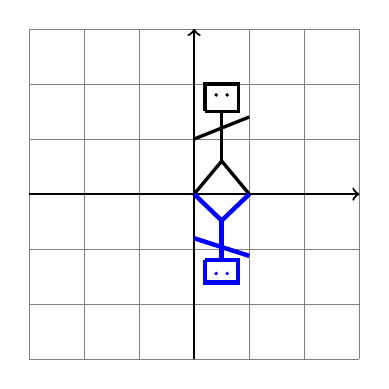
\begin{tikzpicture}[scale=\timyscale]
  \def\timmy{    \draw (0,0)--(0.5,0.6)--(1,0);
    \draw (0.5,0.6)--(0.5,1.5);
    \draw (0,1)--(1,1.4);
    \draw (0.2,1.5) -- (.8,1.5)--(0.8,2)--(0.2,2)-- (0.2,1.5);
    \fill (0.4,1.8) circle (1pt);
    \fill (0.6,1.8) circle (1pt);
}
  \begin{scope}[ultra thin, gray]
    \draw(-3,-3) grid (3,3);
  \end{scope}
  \draw[->, thick](-3,0)--(3,0);
  \draw[->, thick](0,-3)--(0,3);  
  \begin{scope}[very thick]
    \timmy
  \end{scope}
  % \begin{scope}[rotate=90, ultra thick, red]
  %   \timmy
  % \end{scope}  
  \begin{scope}[y=-0.8cm, ultra thick, blue]
    \timmy
  \end{scope}  
  % \begin{scope}[y={(1,1)}, ultra thick, gray]
  %   \timmy
  % \end{scope}  
\end{tikzpicture}
\hfill
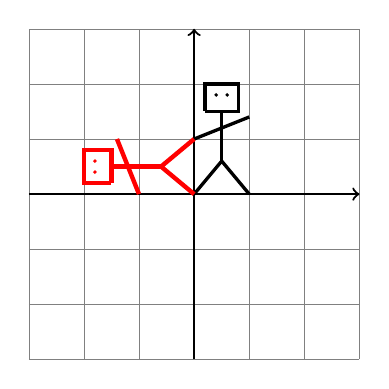
\begin{tikzpicture}[scale=\timyscale]
  \def\timmy{    \draw (0,0)--(0.5,0.6)--(1,0);
    \draw (0.5,0.6)--(0.5,1.5);
    \draw (0,1)--(1,1.4);
    \draw (0.2,1.5) -- (.8,1.5)--(0.8,2)--(0.2,2)-- (0.2,1.5);
    \fill (0.4,1.8) circle (1pt);
    \fill (0.6,1.8) circle (1pt);
}
  \begin{scope}[ultra thin, gray]
    \draw(-3,-3) grid (3,3);
  \end{scope}
  \draw[->, thick](-3,0)--(3,0);
  \draw[->, thick](0,-3)--(0,3);  
  \begin{scope}[very thick]
    \timmy
  \end{scope}
  \begin{scope}[rotate=90, ultra thick, red]
    \timmy
  \end{scope}  
  % \begin{scope}[y=-1cm, ultra thick, blue]
  %   \timmy
  % \end{scope}  
  % \begin{scope}[y={(1,1)}, ultra thick, gray]
  %   \timmy
  % \end{scope}  
\end{tikzpicture}
\hfill
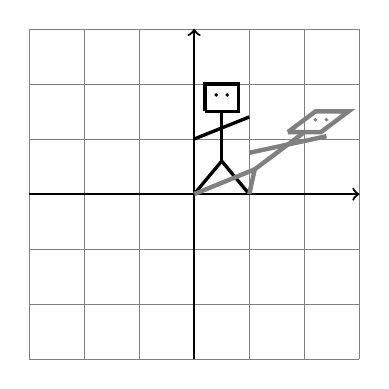
\begin{tikzpicture}[scale=\timyscale]
  \def\timmy{    \draw (0,0)--(0.5,0.6)--(1,0);
    \draw (0.5,0.6)--(0.5,1.5);
    \draw (0,1)--(1,1.4);
    \draw (0.2,1.5) -- (.8,1.5)--(0.8,2)--(0.2,2)-- (0.2,1.5);
    \fill (0.4,1.8) circle (1pt);
    \fill (0.6,1.8) circle (1pt);
}
  \begin{scope}[ultra thin, gray]
    \draw(-3,-3) grid (3,3);
  \end{scope}
  
  \draw[->, thick](-3,0)--(3,0);
  \draw[->, thick](0,-3)--(0,3);  
  \begin{scope}[very thick]
    \timmy
  \end{scope}
  % \begin{scope}[rotate=90, ultra thick, red]
  %   \timmy
  % \end{scope}  
  % \begin{scope}[y=-1cm, ultra thick, blue]
  %   \timmy
  % \end{scope}  
  \begin{scope}[y={(1,.75)}, ultra thick, gray]
    \timmy
  \end{scope}  
\end{tikzpicture}

Poznámka: Stačí si všímat, kam se zobrazují jednotkové vektory ve směru os, tj. kam se zobrazí Timmiho nakročená noha a Timyho ruka, která je natažená dozadu. Případné neceločíselné složky matice jenom odhadněte. \textit{Podle LAFF Linear Algebra - Foundations to Frontiers (www.ulaff.net)}

\reseni

Nakročená noha je v bodě $(1,0)$ a tento bod se transformuje sám na sebe pro krajní obrázky a na bod $(0,1)$ pro prostřední obrázek. Tím je dán první sloupec matice zobrazení. Ruka natažená dozadu je v bodě $(0,1)$ a u modrého Timmyho se transformuje (odhadem) na $(0,-0.8)$, u červeného Timmyho na $(-1,0)$ a u šedého Timmyho (odhadem) na $(1,0.8)$. Matice jsou postupně
\begin{equation*}
  M_{\text{modrá}}=
  \begin{pmatrix}
    1 & 0
    \\
    0 &-0.8
  \end{pmatrix},
\quad
  M_{\text{červená}}=
  \begin{pmatrix}
    0 & -1
    \\
    1 & 0
  \end{pmatrix},\quad
  M_{\text{šedá}}=
  \begin{pmatrix}
    1 & 1
    \\
    0 & 0.8
  \end{pmatrix}.
\end{equation*}

\konec

\subsection{Matice rotace}
Matice rotace o úhel $\theta$ v kladném smyslu je
\begin{equation*}R_\theta=
  \begin{pmatrix}
    \cos\theta & -\sin \theta\\
    \sin\theta & \cos\theta
  \end{pmatrix}.
\end{equation*}
Násobením ověřte, že matice otočení o úhel $-\theta$ je k této matici inverzní.

\textit{Návod:} Funkce kosinus je sudá funkce a funkce sinus je lichá funkce. Proto platí $$\cos(-\theta)=\cos \theta \qquad\text{a}\qquad \sin(-\theta)=-\sin \theta.$$

\textit{Matice rotace je důležitá v aplikacích zabývajících se deformacemi, protože umožní odfiltrovat tu část změny polohy referenčních bodů, která je způsobena rotací a nepřispívá tedy ke změně tvaru tělesa.}

\reseni
Při zkratce $S=\sin \theta$ a $C=\cos\theta$ platí
\begin{equation*}
  R_{-\theta}=\begin{pmatrix} \cos(-\theta) & -\sin(-\theta) \\ \sin(-\theta) & \cos(-\theta)    
  \end{pmatrix}
  =\begin{pmatrix} \cos \theta  & \sin \theta \\ -\sin\theta & \cos\theta    
  \end{pmatrix}
  =
  \begin{pmatrix}
    C & S\\ -S & C
  \end{pmatrix}
\end{equation*}
a potom
\begin{equation*}
  R_\theta R_{-\theta}=
  \begin{pmatrix}
    C & -S \\ S& C
  \end{pmatrix}
  \begin{pmatrix}
    C & S\\ -S & C
  \end{pmatrix}
  =
  \begin{pmatrix}
    C^2+S^2 & CS-SC
\\ SC-CS & S^2+C^2
\end{pmatrix}
=
\begin{pmatrix}
  1 & 0 \\0& 1
\end{pmatrix},
\end{equation*}
kde jsme využili identitu
\begin{equation*}
  \sin^2\theta + \cos^2\theta=1.
\end{equation*}

\konec

\stranka

\subsection{Matice posunutí}
Transformace pomocí násobení matic zachovává počátek a nemůže proto charakterizovat například posunutí roviny. Pokud chceme mít
pomocí maticového násobení realizováno i posunutí, musíme zavést
homogenní souřadnice a ztotožnit bod $(x,y)$ s vektorem
$(x,y,1)^T$. Ukažte, že matice
\begin{equation*}P_{a,b}=
\begin{pmatrix}
  1& 0& a\\
  0 & 1 & b\\
  0& 0& 1
\end{pmatrix}
\end{equation*}
je matice posunutí o $a$ doprava a $b$ nahoru. Odhadněte, jak bude
vypadat matice popisující opačnou transformaci a pro jedno nějaké pořadí
součinu ověřte, že součin těchto matic je jednotková matice.

\reseni
Platí
\begin{equation*}
\begin{pmatrix}
  1& 0& a\\
  0 & 1 & b\\
  0& 0& 1
\end{pmatrix}
\begin{pmatrix}
  x\\y\\1
\end{pmatrix}
=
\begin{pmatrix}
  x+a\\y+b\\1
\end{pmatrix}
\end{equation*}
a vidíme, že k souřadnici $x$ se přičítá $a$ a k souřadnici $y$ se přičítá $b$.
Inverzní zobrazení bude posunutí o $a$ doleva a o $b$ dolů, tj. 
\begin{equation*}
  \begin{pmatrix}
  1& 0& -a\\
  0 & 1 & -b\\
  0& 0& 1
\end{pmatrix}.
\end{equation*}
Přímým výpočtem vidíme, že platí
\begin{equation*}
  \begin{pmatrix}
  1& 0& a\\
  0 & 1 & b\\
  0& 0& 1
\end{pmatrix}
  \begin{pmatrix}
  1& 0& -a\\
  0 & 1 & -b\\
  0& 0& 1
\end{pmatrix}=
  \begin{pmatrix}
  1& 0& 0\\
  0 & 1 & 0\\
  0& 0& 1
\end{pmatrix}.
\end{equation*}

\konec

\stranka

\subsection{Matice, zachovávající význačné směry} Dřevo má tři výrazné
směry a pokud máme možnost zvolit souřadnou soustavu tak, aby tyto
směry byly dány vektory $(1,0,0)^T$, $(0,1,0)^T$ a $(0,0,1)^T$, formulace
fyzikálních zákonů se zjednoduší. Najděte
\begin{enumerate}
\item  nejobecnější matici $3\times 3$, která zachovává směr vektoru $(1,0,0)^T$,
\item  nejobecnější symetrickou matici $3\times 3$, která zachovává směr vektoru $(1,0,0)^T$,
\item  nejobecnější symetrickou matici $3\times 3$, která zachovává směr vektorů $(1,0,0)^T$, $(0,1,0)^T$, $(0,0,1)^T$.
\end{enumerate}

\textit{V tomto příkladě uvidíme, že matice zachovávající směr os souřadnic jsou v určitém smyslu pěkné.}

\reseni
ad 1.
\begin{equation*}
  \begin{pmatrix}
    a & b & c \\ d & e & f \\ g& h& i \end{pmatrix}
  \begin{pmatrix}
    1\\0\\0
  \end{pmatrix}
  =
  \begin{pmatrix}
    a \\ d \\g
  \end{pmatrix}
\end{equation*}
a vektory $(1,0,0)^T$
a $(a,d,g)^T$ musí mít stejný směr. Proto $d=g=0$ a nejobecnější matice s danou vlastností je matice, která ve druhém a třetím řádku začíná nulou.
\begin{equation*}
    \begin{pmatrix}
    a & b & c \\ 0 & e & f \\ 0& h& i \end{pmatrix}
\end{equation*}

ad 2. Jako minulý případ, ale aby byla matice symetrická, musí být také $b=c=0$, a $h=f$ tj.
\begin{equation*}
    \begin{pmatrix}
    a & 0 & 0 \\ 0 & e & f \\ 0& f& i \end{pmatrix}.
\end{equation*}

ad 3. Jako minulý případ, ale ještě se musí zachovávat směry vektorů $(0,1,0)^T$ a $(0,0,1)^T$. Platí
\begin{equation*}
    \begin{pmatrix}
    a & 0 & 0 \\ 0 & e & f \\ 0& f& i \end{pmatrix}
  \begin{pmatrix}
    0 \\1\\0
  \end{pmatrix}
  =
  \begin{pmatrix}
    0 \\ e\\f
  \end{pmatrix}
,\quad
    \begin{pmatrix}
    a & 0 & 0 \\ 0 & e & f \\ 0& f& i \end{pmatrix}
  \begin{pmatrix}
    0 \\0\\1
  \end{pmatrix}
  =
  \begin{pmatrix}
    0 \\ f\\i \end{pmatrix}
\end{equation*}
a aby vzor a obraz měly stejný směr, musí být $f=0$. Nejobecnější symetrická matice, která zachovává směr všech tří základních bázových vektorů je matice, která má mimo hlavní diagonálu nuly.
\konec



\stranka

\subsection{Matice derivování}
Ukažte, že matice 
$A=
\begin{pmatrix}
  0 & 0 & 0 \\
  2 & 0 & 0 \\
  0 & 1 & 0
\end{pmatrix}
$
je matice derivování polynomů stupně nejvýše $2$, pokud polynom $ax^2+bx+c$ ztotožníme s vektorem $
\begin{pmatrix}
  a \\ b\\c
\end{pmatrix}
$.  Vysvětlete, jak bychom
interpretovali matici $A^2$ a $A^3$ a tyto matice vypočtěte.

\textit{Návod: je možné ukázat buď pro obecný polynom $ax^2+bx+c$, nebo samostatně pro polynomy  $x^2$, $x$ a $1$ a poté si všimnout, že ostatní polynomy můžeme dostat lineárními kombinacemi a maticová násobení tyto lineární kombinace nepokazí díky tomu, že je distributivní a komutuje při násobení s konstantou.
 V tomto příkladě mimo jiné vidíme, že mocnina nenulové matice může být nula. To je efekt, který nemá obdobu u násobení reálných čísel.}


\reseni Polynom $x^2$ má derivaci $2x$, tj. v označení pomocí vektorů
se musí vektor $(1,0,0)^T$ zobrazit na $(0,2,0)^T$. Toto snadno
ukážeme, že platí, protože se vlastně jedná o první sloupec matice
$A$. Podobně, polynom $x$ má derivaci $1$ a polynom $1$ má derivaci
$0$, tj. v označení pomocí vektorů se musí vektory $(0,1,0)^T$ a
$(0,0,1)^T$ zobrazit na $(0,0,1)^T$ a $(0,0,0)^T$. Opět vidíme snadno,
že pro naši matici $A$ platí (dostáváme vlastně druhý a třetí sloupec
matice $A$).

Protože libovolný polynom druhého stupně dostaneme pomocí lineárních
kombinací výše uvedených vektorů a protože tyto lineární kombinace
zůstanou při maticovém násobení zachovány, je při výše definovaném
zobrazení obrazem libovolného polynomu druhého stupně jeho derivace.

Pro obecný polynom $ax^2+bx+c$ s derivací $2ax+b$ vidíme, že obrazem
vektoru $(a,b,c)^T$ musí být $(0,2a, b)^T$, což matice $A$ opět (po
krátkém výpočtu) splňuje.

Matice $A^2$ je druhá derivace a $A^3$ třetí derivace a mají tvar
\begin{equation*}
  A^2=
  \begin{pmatrix}
  0 & 0 & 0 \\
  0 & 0 & 0 \\
  2 & 0 & 0
\end{pmatrix}, \qquad
  A^3=
  \begin{pmatrix}
  0 & 0 & 0 \\
  0 & 0 & 0 \\
  0 & 0 & 0
\end{pmatrix}.
\end{equation*}


\konec


\stranka

\subsection{Matice projekce}
Matice $P=
\begin{pmatrix}
  \cos^2 \alpha & \cos \alpha \sin \alpha \\
  \cos\alpha\sin\alpha & \sin^2 \alpha
\end{pmatrix}
$ reprezentuje kolmou projekci na přímku, která jde počátkem soustavy souřadnic a svírá s kladnou částí osy $x$ úhel $\alpha$.
\begin{enumerate}
\item Ukažte, že platí $P^2=P$. To znamená, že body na přímce se
  zobrazí samy na sebe.
\item Ukažte, (nemusíte výpočtem, například graficky, nebo využitím
  toho, že každý bod přímky se zobrazí sám na sebe) že dva různé body
  se projekcí mohou zobrazit na stejný bod a proto není naděje na to
  mít inverzní zobrazení. Proto neexistuje inverzní matice.
\end{enumerate}

\reseni
Pro $C=\cos \alpha$ a $S=\sin\alpha$ dostáváme
\begin{equation*}
  \begin{aligned}
P^2&=
  \begin{pmatrix}
    C^2 & CS \\CS & S^2
  \end{pmatrix}
  \begin{pmatrix}
    C^2 & CS \\CS & S^2
  \end{pmatrix}
=
\begin{pmatrix}
  C^4+C^2S^2 & C^3S+CS^3 \\
C^3S+CS^3 & C^2S^2+S^4
\end{pmatrix}
\\&=
\begin{pmatrix}
  C^2(C^2+S^2) & CS(C^2+S^2) \\
CS(C^2+S^2) & S^2(C^2+S^2)
\end{pmatrix}
=
\begin{pmatrix}
  C^2 & CS \\
CS & S^2
\end{pmatrix}
=P
\end{aligned}
\end{equation*}

Evidentně jakýkoliv bod mimo přímku projekce a jeho obraz jsou da různé body, které mají stejný obraz. Proto nemůže existovat inverzní zobrazení.

Pro determinant platí
\begin{equation*}
  |P|=
  \begin{vmatrix}
      C^2 & CS \\
CS & S^2
  \end{vmatrix}
=C^2S^2-(CS)(CS)=C^2S^2-C^2S^2=0
\end{equation*}
a tento výpočet potvrzuje, že neexistuje inverzní matice.
\konec


\stranka
\section{Determinanty, soustavy rovnic}

\stranka
\subsection{Určete následující determinanty}

\begin{enumerate}
\item $D_1=
  \begin{vmatrix}
    2 & -1 \\ 4 &3
  \end{vmatrix}
  $
\item $D_2=
  \begin{vmatrix}
    2 & -1 \\ x-4 &y-3
  \end{vmatrix}
  $

  ($D_2=0$ je přímka daná bodem $(4,3)$ a směrovým vektorem $(2,-1)$)
\item $D_3=
  \begin{vmatrix}
    2-\lambda & -1 \\ 4 & 3-\lambda
  \end{vmatrix}
  $ (charakteristický polynom matice z prvního bodu)
\item
  $D_4=
  \begin{vmatrix}
    1 & -1 & 0\\ 2 & 3 & 1 \\ -1 &-1 & 2\end{vmatrix}
  $
\item
  $D_5=
  \begin{vmatrix}
    a & -1 & 0\\ 2 & 3 & 1 \\ -1 &-1 & 2\end{vmatrix}
  $  
\item
  $D_6=
  \begin{vmatrix}
    2-\lambda & 0 & 0\\ 0 & 3-\lambda & 0 \\ 0 & 0& 7-\lambda \end{vmatrix}
  $  (charakteristický polynom diagonální matice)
\end{enumerate}


\reseni

\begin{equation*}
  \begin{aligned}
    D_1&=2\cdot 3 - (-1)\cdot 4=6+4=10\\
    D_2&=2\cdot(y-3)-(-1)\cdot (x-4)=2y-6+x-4=x+2y-10\\
    D_3&=(2-\lambda)\cdot(3-\lambda)-(-1)\cdot 4 = \lambda^2-5\lambda+10\\
    D_4&=12\\
    D_5&=7a+5\\
    D_6&=(2-\lambda)(3-\lambda)(7-\lambda)
\end{aligned}
\end{equation*}

\konec



\stranka


\subsection{Soustava lineárních rovnic s jediným řešením} Vyřešte soustavu rovnic.

\shorthandoff{-}
\begin{equation*}
  \begin{pmatrix}
1 &2 &2 \\
2 &2 &-1\\
2 &3 &1 \\
\end{pmatrix}
\begin{pmatrix}
  x_2\\x_2\\x_3
\end{pmatrix}
=
\begin{pmatrix}
  3\\1\\-1
\end{pmatrix}
\end{equation*}


\textit{Soustava rovnic je asi nejdůležitější aplikace lineární algebry, ale v dnešním světě není důvod ji řešit ručně. Je však užitečné si alespoň základní manipulace vyzkoušet na jednoduchém příkladě. Tento moc času nezabere.}



\stranka
\subsection{Soustava lineárních rovnic s nekonečně mnoha řešeními} Vyřešte soustavu rovnic.

\begin{equation*}
  \begin{pmatrix}
3 &-1 &-1 &-1\\ 
2 &1 &1 &-2 \\
1 &-2 &-2 &1 \\
3 &-1 &-1 &1 \\
\end{pmatrix}
\begin{pmatrix}
  x_1 \\ x_2 \\x_3\\x_4
\end{pmatrix}
=
\begin{pmatrix}
  0 \\ 0 \\0\\0
\end{pmatrix}
\end{equation*}

\textit{Soustava s nekonečně mnoha řešeními typicky vychází při
  hledání vlastních čísel matice. Na tomto příkladě si osaháme případ
  homogenní soustavy a jednoparametrického řešení, tj. případ, který
  při výpočtu vlastních vektorů vychází nejčastěji.}


\subsection{Soustava lineárních rovnic s parametrem}
Pro jakou hodnotu parametru má soustava nekonečně mnoho řešení?

\stranka


\stranka
\section{Hlavní cvičení}
Cvičení ve středu ani ve čtvrtek se nekoná kvůli hlavnímu cvičení. Přednáška je beze změny.


\stranka
\section{Vlastní čísla a směry}



\stranka
\subsection{Vlastní čísla a vektory matice $2\times 2$}

Uvažujme symetrickou matici
\begin{equation*} A=
  \begin{pmatrix}
  3 & 1\\
  1 & 3
\end{pmatrix}.
\end{equation*}
\begin{enumerate}
\item Určete vlastní čísla a jednotkové vlastní vektory této matice.
\item Sestavte matici $P$ tak, aby ve sloupcích obsahovala jednotkové vlastní vektory.
Pokud je to možné, napište matici $P$ tak, aby její determinant byl kladný.
\item Ověřte, že  $P^TAP=D$  je diagonální matice.
\end{enumerate}
\textit{Návod: Vlastní vektory příslušné různým vlastním číslům jsou na sebe kolmé.}

\reseni
Charakteristický polynom je
\begin{equation*}
  \begin{vmatrix}
    3-\lambda & 1\\1 & 3-\lambda
  \end{vmatrix}
  =(3-\lambda)^2-1=9-6\lambda+\lambda^2-1=\lambda^2-6\lambda+8=(\lambda-4)(\lambda-2)
\end{equation*}
a vlastní čísla jsou $\lambda_1=2$ a $\lambda_2=4$.
Protože platí
\begin{equation*}
A-\lambda_1 I
  =  \begin{pmatrix}
    3-2 & 1 \\
    1 &3-2
  \end{pmatrix}
  =
    \begin{pmatrix}
    1 & 1 \\
    1 &1
  \end{pmatrix},
\end{equation*}
je vlastní vektor příslušný vlastní hodnotě $\lambda_1$ řešením soustavy
\begin{equation*}
\begin{pmatrix}
    1 & 1 \\ 1 &1
  \end{pmatrix}
\begin{pmatrix}
  x_1\\x_2
\end{pmatrix}
=
  \begin{pmatrix}
    0\\0
  \end{pmatrix}
\end{equation*}
To je vlastně dvakrát zopakovaná rovnice
\begin{equation*}
  x_1+x_2=0,
\end{equation*}
která má řešení například $x_1=1$ a $x_2=-1$. Protože délka vektoru $(1,-1)$ je $\sqrt{1^2+(-1)^2}=\sqrt 2$, jednotkový vlastní vektor je $e_1=\left(\frac 1{\sqrt 2}, -\frac 1 {\sqrt 2}\right)^T$. Podobně by se dal najít jednotkový vlastní vektor příslušný druhé vlastní hodnotě, ale protože oba vektory musí být na sebe kolmé, stačí vzít jednotkový vektor, který je k $e_1$ kolmý, například
$e_2=\left(\frac 1{\sqrt 2}, \frac 1 {\sqrt 2}\right)^T$. Matici $P$ můžeme vzít
s $e_1$ v prvním a $e_2$ druhém sloupci, tj.
\begin{equation*}
    P=  \begin{pmatrix}
      \frac 1{\sqrt 2} & \frac 1{\sqrt 2}\\
      -\frac {1}{\sqrt 2} & \frac 1{\sqrt 2}
    \end{pmatrix}.
  \end{equation*}
  Rychlý výpočet ukazuje, že matice $P$ má determinant roven jedné. Kdyby vyšel roven minus jedné, stačí prohodit sloupce nebo jeden sloupec vynásobit faktorem $-1$.
  
Pokud ještě před násobením matic vytkneme opakující se faktor z obou matic, násobením dostáváme
\begin{equation*}
  \begin{aligned}
  P^TAP&=\begin{pmatrix}
      \frac 1{\sqrt 2} & -\frac 1{\sqrt 2}\\
      \frac {1}{\sqrt 2} & \frac 1{\sqrt 2}
    \end{pmatrix}
        \begin{pmatrix}
    3 & 1 \\ 1 &3
  \end{pmatrix}
  \begin{pmatrix}
      \frac 1{\sqrt 2} & \frac 1{\sqrt 2}\\
      -\frac {1}{\sqrt 2} & \frac 1{\sqrt 2}
    \end{pmatrix}\\&
    =\frac 1{\sqrt 2}\frac 1{\sqrt 2}
    \begin{pmatrix}
      1 & -1 \\ 1 &1
    \end{pmatrix}
        \begin{pmatrix}
    3 & 1 \\ 1 &3
  \end{pmatrix}
    \begin{pmatrix}
      1 & 1 \\ -1 &1
    \end{pmatrix}
    \\&=
    \frac 1{2}
    \begin{pmatrix}
      1 & -1 \\ 1 &1
    \end{pmatrix}
    \begin{pmatrix}
      2 & 4 \\-2 & 4
    \end{pmatrix}
    \\&=
    \frac 1{ 2}
    \begin{pmatrix}
      4& 0 \\ 0& 8
    \end{pmatrix}=
    \begin{pmatrix}
      2& 0 \\0& 4
    \end{pmatrix}.
  \end{aligned}
\end{equation*}
Podle očekávání vyšla diagonální matice s vlastními hodnotami v hlavní diagonále.
 \konec

% \stranka

% \section{Komentář k předchozímu} Zobrazení popsané maticí $A$
% je naznačeno na obrázku a jak vidno, mění tvar modrého jednotkového čtverce.

% \hbox to \hsize{\begin{minipage}[t]{0.35\linewidth}\vspace*{0pt}
% \begin{tikzpicture}[scale=1]
%   \draw[-latex](0,0)--(3,0);
%   \draw[-latex](0,0)--(0,1.5);

%   \fill[blue, opacity=0.5] (0,0) rectangle (1,1);
%   \fill[red, opacity=0.5] (0,0) -- (3,-1) -- (2,0) -- (-1,1) -- cycle;
%   \draw[ultra thick,blue,-latex] (0,0)--(1,1) node[right] {$u$};
%   \draw[ultra thick,red,-latex] (0,0)--(2,0) node[above right] {$u'$};

%   \draw[ultra thick,blue,-latex] (0,0)--(0,1) node[right] {$v$};
%   \draw[ultra thick,red,-latex] (0,0)--(-1,1) node[above right] {$v'$};
%   \draw (-0.5,1.7) node [right, gray] {\footnotesize Vzor je modře, obraz červeně.};
% \end{tikzpicture}

% Vektor $u$ se při zobrazení otočí po směru a $v$ proti směru
% hodinových ručiček. Někde mezi nimi bude vektor, který při zobrazení
% směr nemění. To bude vlastní vektor a z obrázku je možné odhadnout, že
% bude příslušný menší vlastní hodnotě.
% \end{minipage}\hfil\vrule\hfil
% \begin{minipage}[t]{0.62\linewidth}\vspace*{-10pt}
%   \begin{tikzpicture}[scale=1]
%       \draw (1.2,1.2) node [right,gray, text width=4cm] {\footnotesize Vzor je vybarven, obraz je znázorněn jenom obrysem, barvy obrazu a vzoru si odpovídají.};
%   \draw[-latex](0,0)--(3,0);
%   \draw[-latex](0,0)--(0,1.5);

%   \fill[blue, opacity=0.5] (0,0) rectangle (1,1);
%   \draw[ultra thick, blue] (0,0) -- (3,-1) -- (2,0) -- (-1,1) -- cycle;

%   \fill[green, opacity=0.5] (0,0)--(0.382683432365090,0.923879532511287)--
%   (-0.541196100146197, 1.30656296487638) --
%   (-0.923879532511287,0.382683432365090)--cycle;

%   \draw[ultra thick, green]  (0,0)--(0.224170764583983, 0.541196100146197)--(-2.93015126531497, 1.84775906502258)-- (-3.15432202989895, 1.30656296487638) -- cycle;
% \end{tikzpicture}

% Zobrazení symetrickou maticí $A$ uvažovanou v tomto příkladě si můžeme představit tak, že máme elastickou pásku, která se působením síly deformuje tak, že se natahuje v jednom směru a zužuje v příčném směru. Čtverec nakreslený na pásce tak, že jeho strany leží v těchto směrech (zelený) se deformuje na obdélník. Obecný čtverec (modrý) se deformuje tak, že se mění úhly. Na přednášce jsme si naznačili, jak se ukáže, že deformace v těchto směrech je extremální, vrátíme se k~tomu v záverečném shrnutí na konci semestru, protože jde o kombinaci úlohy z lineární algebry a diferenciálního počtu.

% \end{minipage}}


\stranka
\subsection{Neceločíslená vlastní čísla a vektory matice $2\times 2$}

 
\stranka
\subsection{Vlastní čísla a vektory matice $3\times 3$.}

V minulém cvičení jsme ukázali, že nejobecnější symetrická matice zachovávající směr vektoru  $(1,0,0)^T$ má v prvním řádku a prvním sloupci jenom jeden nenulový prvek, prvek v hlavní diagonále.

Uvažujme matici
\begin{equation*}
A=  \begin{pmatrix}
  5 & 0 & 0\\
  0 & 2 & 2\\
  0 & 2 & 5
\end{pmatrix},
\end{equation*}
která je tohoto typu.
Určete vlastní čísla a zbylé vlastní vektory matice.


\reseni
Podle zadání víme, že jeden z vlastních vektorů je $e_1=(1,0,0)^T$ a protože se zobrazí na pětinásobek, je příslušná vlastní hodnota $\lambda_1=5$. Charakteristický polynom je
\begin{equation*}
  \begin{aligned}
  \begin{vmatrix}
  5-\lambda & 0 & 0\\
  0 & 2-\lambda & 2\\
  0 & 2 & 5-\lambda
\end{vmatrix}
&=(5-\lambda)(2-\lambda)(5-\lambda)-(5-\lambda)\times 2\times 2\\& =
(5-\lambda)\Bigl[(2-\lambda)(5-\lambda) -4\Bigr]
\\&=(5-\lambda)(\lambda^2 -7\lambda +6)
=(5-\lambda)(\lambda-1)(\lambda-6)
\end{aligned}
\end{equation*}
Další dvě vlastní hodnoty jsou $\lambda_2=1$ a $\lambda_3=6$

Uvažujme matici
\begin{equation*}
  A-1 I=
  \begin{pmatrix}
    4 & 0 & 0\\
    0 & 1 & 2\\
    0 & 2& 4
  \end{pmatrix}.
\end{equation*}
Soustava
\begin{equation*}
  \begin{pmatrix}
    4 & 0 & 0\\
    0 & 1 & 2\\
    0 & 2& 4
  \end{pmatrix}
  \begin{pmatrix}
    x_1\\x_2\\x_3
  \end{pmatrix}
  =
  \begin{pmatrix}
    0 \\0\\0
  \end{pmatrix}
\end{equation*}
má řešení $x_1=0$ (plyne z první rovnice) a například $x_2=2$ a $x_3=-1$ (plyne z druhé a třetí rovnice, které jsou jedna násobkem druhé). Vlastní vektor příslušný vlastní hodnotě $\lambda_2=1$ je $e_2=(0,2,-1)^T$.

Uvažujme matici
\begin{equation*}
  A-6 I=
  \begin{pmatrix}
    -1 & 0 & 0\\
    0 & -4 & 2\\
    0 & 2& -1
  \end{pmatrix}.
\end{equation*}
Soustava
\begin{equation*}
  \begin{pmatrix}
    -1 & 0 & 0\\
    0 & -4 & 2\\
    0 & 2& -1
  \end{pmatrix}
  \begin{pmatrix}
    x_1\\x_2\\x_3
  \end{pmatrix}
  =
  \begin{pmatrix}
    0 \\0\\0
  \end{pmatrix}
\end{equation*}
má řešení $x_1=0$ (plyne z první rovnice) a například $x_2=1$ a $x_3=2$ (plyne z druhé a třetí rovnice, které jsou jedna násobkem druhé). Vlastní vektor příslušný vlastní hodnotě $\lambda_3=6$ je $e_3=(0,1,2)^T$.

\konec



\subsection{Transformace tenzoru pootočením}

\subsection{Extrémy diagonálních prvků transformovaného tenzoru}



\stranka
\section{Parciální derivace, rovnice vedení tepla}

\stranka
\subsection{Stacionární vedení tepla, lineární materiál}

Najděte rozložení teploty v homogenní stěně při stacionárním vedení tepla a v materiálu s lineární materiálovou odezvou (koeficient tepelné vodivosti je konstantní).
Jinými slovy, najděte všechny funkce splňující
$$\frac{\partial}{\partial x} \left(k \frac{\partial T}{\partial x}\right)=0$$
pro $T=T(x)$ a $k\in \mathbb R^+$.

\textit{Poznámka: Výsledek se dá použít i pro stěnu složenou z různých vrstev. Postupuje se tak, že se jednotlivé vrstvy nahradí ekvivalentními vrstvami z jednoho materiálu. Například vrstva z materiálu s polovičním koeficientem tepelné vodivosti se nahradí vrstvou, která je dvojnásobně silná.}

\textit{Poznámka: Na stejnou úlohu se stejnou rovnicí a stejným řešením vede například proudění podzemní vody ve zvodni s napjatou hladinou (představou může být podzemní voda protékající půdou a shora i zdola ohraničená nepropustnou vrstvou).}

\reseni

Rovnici můžeme vydělit konstantou $k$

Po zintegrování dostáváme $$ \frac{\partial T}{\partial x}=C_1$$
a po dalším zintegrování $$T=C_1x+C_2.$$ Teplota se mění lineárně. Dvě konstanty se určí pomocí dvou teplot na hranicích stěny.

\konec

\stranka
\subsection{Stacionární vedení tepla, nelineární materiál}


Najděte rozložení teploty v homogenní stěně při stacionárním vedení
tepla a v materiálu s nelineární materiálovou odezvou (koeficient
tepelné vodivosti není konstantní).  Použijte lineární závislost
koeficientu tepelné vodivosti na teplotě.  Jinými slovy, najděte
všechny funkce splňující
$$\frac{\partial}{\partial x} \left(k \frac{\partial T}{\partial x}\right)=0$$
pro $T=T(x)$ a $k=a+bT$, $a,b\in \mathbb R$.

\textit{Poznámka: Výpočet necháme kvalitativní abychom viděli, že teplotní profil ve stěně není lineární. Pro užitečnost v inženýrských aplikacích je vhodné přidat okrajové podmínky a vyjádřit řešení pomocí parametrů v těchto okrajových podmínkách. To jsou typicky teploty na jednotlivých stranách stěny.}

\textit{Poznámka: Na stejnou úlohu se stejnou rovnicí a stejným řešením, pouze pro $a=0$, vede například proudění podzemní vody ve zvodni s volnou hladinou (narozdíl od předchozího příkladu chybí horní nepropustná vrstva).}

\reseni
Po zintegrování dostáváme
$$(a+bT)\frac{\partial T}{\partial x}=C_1$$
a rovnici řešíme jako diferenciální rovnici se separovanými proměnnými.
Odseparováním získáme
$$(a+bT)\mathrm dT=C_1\mathrm dx$$
a po zintegrování
$$aT+\frac 12bT^2 = C_1x+C_2.$$
Řešením je
parabola otočená naležato. Dvě konstanty se určí pomocí teplot na hranicích stěny. Pro správný profil je nutné si vybrat
správnou část paraboly tak, aby teplota zůstala mezi teplotami na
krajích stěny.
\konec


\subsection{Výpočet  parciálních derivací}

\newcommand\pd[2][x]{\frac{\partial }{\partial #1}\left(\vphantom {\frac 22}#2\right)}
\begin{multicols}2
\begin{enumerate}[a)]
\item $\pd{x^2y+2xy^3+x+1}$
\item $\pd[y]{x^2y+2xy^3+x+1}$
\item $\pd{3x(3-x-2y)}$
\item $\pd[y]{3x(3-x-2y)}$
\end{enumerate}
\end{multicols}

\reseni
\begin{enumerate}[a)]
\item $\pd{x^2y+2xy^3+x+1}=2x\cdot y+2y^3+1+0=2xy+2y^3+1$
\item $\pd[y]{x^2y+2xy^3+x+1}=x^2+2x\cdot 3y^2+0+0=x^2+6xy^2$
\item $\pd{3x(3-x-2y)}=\pd{9x-3x^2-6xy}=9-3\cdot 2x-6\cdot 1\cdot y=9-6x-6y$
\item $\pd[y]{3x(3-x-2y)}=\pd[y]{9x-3x^2-6xy}=0-0-6x=-6x$
\end{enumerate}

\konec

%\subsection{Gradient, anizotropní vedení tepla}

%\obrazek{teplo_deska.png}
\subsection{Rovnice vedení tepla v dvourozměrném materiálu}

%sage: x,y = var('x,y')
%sage: contour_plot((x+2*y)^2+x^3, (x,0,10), (y,0,10), contours=15, cmap="coolwa%rm", plot_points=150, colorbar=True)

Teplota ve dvourozměrné desce pro $0\leq x\leq 10$ a $0\leq y\leq 10$ zachycené v určitém okamžiku termokamerou je popsána rovnicí
  $$T(x,y)=(x+2y)^2+x^3.$$
  Rozměry jsou v centimetrech, teplota ve stupních Celsia. (Formálně to nevychází, ale ke každému členu můžeme dodat konstantu, která rozměr opraví tak, aby výsledek opravdu vycházel ve stupních Celsia. Pro jednoduchost tuto komplikaci vynecháme.)

\begin{enumerate}
\item Vypočtěte gradient $\nabla T$  a tok tepla $-\lambda \cdot \nabla T.$
Součinitel tepelné vodivosti (pro jednoduchost s celými čísly a bez jednotky) je $\lambda=
  \begin{pmatrix}
    5 & 1\\1&4
  \end{pmatrix}.
$ 
\item Určete, zda na levém okraji desky ($x=0$) teče teplo dovnitř desky nebo z desky ven.
\item Vypočtěte divergenci toku tepla, tj. $\nabla\cdot(-\lambda \cdot \nabla T).$
\item V desce nejsou zdroje tepla. Ochlazuje se deska uprostřed, nebo otepluje?
\end{enumerate}


\stranka
\subsection{Stacionární vedení tepla v žebru chladiče}

\subsection{Difuzní rovnice ve 2D}

\stranka
\section{Dvojný integrál}

\subsection{Kvadratický moment obdélníku}

\subsection{Těžiště trojúhelníku}

\subsection{Velikost tlakové síly na přehradu}

\subsection{Působiště tlakové síly na přehradu}

\stranka
\section{Shrnutí}

Dle časových možností a průběhu semestru: shrnutí nebo opakování nebo výpočet ukázkové písemky nebo rezerva pro případ rektorského nebo děkanského volna, rezerva pro případ státních svátků apod.


%\endinput


\stranka


\section{Archiv}

\stranka
\obrazek[http://ecoursesonline.iasri.res.in]{aq.png}[-10pt]


\subsection{Pokles hladiny podzemní vody při ustáleném rovinném proudění}

\label{pokles}
Stavovou veličinou pro popis podzemní vody je \textit{piezometrická
  hladina} $h$ měřená v metrech (hrubá představa může být hladina
spodní vody nebo, v případě že je shora ohraničení nepropustnou
vrstvou, tak hladina, kam by vystoupila voda ve vrtu). Prostor, kde
voda teče, se nazývá \textit{zvodeň} (aquifer).
Proudění řídí \textit{Darcyho zákon}, který
  vyjadřuje, že \textit{filtrační rychlost} $v_f$ podzemní vody je úměrná
  sklonu piezometrické hladiny, tj. rychlosti, s jakou klesá
  piezometrická hladina jako funkce $x$.

  \vspace*{-15pt}
\begin{enumerate}[A)]\itemsep 0 pt
\item Zapište Darcyho zákon kvantitativně pomocí derivace piezometrické hladiny. 
\item Tok je dán součinem filtrační rychlosti a obsahu plochy kolmo na
  rychlost. Uvažujte obdélníkovou plochu $h\times 1$, která je na výšku přes celou
  zvodnělou vrstvu $h$ a na šířku má jednotkovou délku. Vynásobte její obsah 
  filtrační rychlostí a dostanete \textit{průtok na jednotku šířky}, označovaný
  $q$. Pro ustálené proudění je $q$ konstantní.
\item Výsledný vztah z předchozího bodu chápejte jako diferenciální rovnici s neznámou funkcí $h$ jako funkcí $x$ a řešením rovnice najdete křivku snížení hladiny podzemní vody v podélném profilu. 
\end{enumerate}

(\textit{Podle Dana Říhová a Jana Marková, Poznámky k přednáškám z Hydrauliky, přednáška č. 9.})

\reseni

\begin{enumerate}[A)]
  \item  $$v_f=-k\derivace {h}x$$
  \item $$q=-kh\derivace hx$$
  \item $$
    \begin{aligned}
      q\,\mathrm{d}x&=-kh\,\mathrm dh\\
      \int q\,\mathrm{d}x&=-k \int h\,\mathrm dh\\
      qx&=-\frac k2 h^2+C
    \end{aligned}
    $$
    V souřadnicích, kdy osa $x$ směřuje doprava a $h$ nahoru, se jedná
    se o parabolu ``otočenou vrcholem směrem doprava''.
\end{enumerate}
\konec



\obrazek[http://ecoursesonline.iasri.res.in]{well.png}[-25pt]


\subsection{Studna s volnou hladinou}

Uvažujme diferenciální rovnici
\begin{equation}
q=-kh\derivace hx \tag{*}\label{*}
\end{equation}
odvozenou v \ref{pokles} B. Tentokrát budeme studovat studnu s volnou hladinou\footnote{Zjednodušeně, voda ve studni je na úrovni hladiny podzemní vody. Studna nevznikla navrtáním nepropustné vrstvy, kdy by byla voda natlakovaná a vystoupila do výšky odpovídající tomuto tlaku.} Je-li studna čerpána konstantní rychlostí $Q$, je tok na jednotku délky na kružnici o poloměru $x$ roven $q=-\frac {Q}{2\pi x}$ (voda teče dovnitř, tj. ve směru ve kterém klesá $x$). Dosaďte tento vztah do rovnice \eqref{*} a rovnici vyřešte s počáteční podmínkou $h(R)=H$, kde $H$ odpovídá hladině vody ve studni a $R$ je poloměr studny (na obrázku $h_w$ a $r_w$). Dostanete rovnici \textit{snížení hladiny v okolí studny} čerpané rychlostí $Q$ (depresní křivka).
(\textit{Volně podle Dana Říhová a Jana Marková, Poznámky k přednáškám z Hydrauliky, přednáška č. 9. Analogickým způsobem se počítají tepelné ztráty při prostupu tepla válcovou stěnou (viz \url{https://youtu.be/rvyogmaUmUQ}).})


\reseni
$$
\begin{aligned}
  -\frac{Q}{2\pi x}&=-kh\derivace hx\\
%  \frac{Q }{2\pi x}\,\mathrm {d}x&=kh\,\mathrm d h\\
  \frac{Q }{2\pi} \int \frac{\mathrm {d}x}{x}&=k\int h\,\mathrm d h\\
  \frac{Q }{2\pi}\ln x&=k \frac {h^2}2 +c\\
\text{obecné řešení: }  \frac{Q }{\pi}\ln x&=k {h^2} +C\\
\text{z počáteční podmínky: }  \frac{Q }{\pi}\ln R&=k {H^2} +C\\
  C&=\frac{Q }{\pi}\ln R-k {H^2}\\
\text{po dosazení do obecného řešení: }   \frac{Q }{\pi}\ln x&=k {h^2} +\frac{Q }{\pi}\ln R-k {H^2}\\
\text{po úpravě: }  \frac{Q }{k\pi}\ln \frac {x}{R}&={h^2} - {H^2}\\
\end{aligned}
$$
Tento vztah umožňuje například navrhnout průměr studny, odhadnout
vydatnost studny, nebo pomocí odčerpávaného vrtu a menších pomocných
vrtů sledujících pokles hladiny v okolí odčerpávaného vrtu stanovit
filtrační součinitel $k$. Využití vzorce
\begin{equation*}
  \frac{Q }{k\pi}\ln \frac {x}{R}={h^2} - {H^2}
\end{equation*}
je však mnohem rozmanitější,
umožňuje vypočítat poměry ve stavebních jámách a v jejich okolí. To je
užitečné například při odhadu, kolik vody se hromadí ve výkopu. Další
využití je, že dokážeme odhadnout vliv stavební jámy na hydrologické
poměry v okolí a tyto poměry dokážeme měnit a přizpůsobovat našim
potřebám. Častou aplikací je například hydraulická clona (soustava
prvků rozmístěných a provozovaných tak, aby nedocházelo k šíření kontaminace z chemické výroby do vodárensky využívaných vod).

\konec


\stranka


\obrazek{kluzak.jpg}
\subsection{Rychlost klesání kluzáku}
Teplota klesá s výškou o $2^\circ \mathrm C$ na kilometr. Pilot
kluzáku vidí, že teplota v okolí jeho kluzáku roste rychlostí
$10^{-3}{}^\circ \mathrm C/\mathrm{s}$. Vyjádřete tato pozorování pomocí
derivací a určete, jak rychle ztrácí kluzák výšku. Návod: Uvažujte složenou funkci $T(h(t))$ a hledejte její derivaci podle času.

\textit{Tento příklad ukazuje, že pravidlo pro derivaci složené funkce je logické. V tomto případě vlastně přepočítává klesání z jednotek stupně Celsia za sekundu na jednotky kilometr výšky za sekundu. Můžete si to zkusit na prstech nebo pomocí trojčlenky a dojdete k tomu stejnému, k čemu pomocí derivace funkce. Při měnících se rychlostech výpočet pomocí trojčlenky použitelný není, pravidlo pro derivaci složené funkce je však k dispozici vždy.}

\reseni
Je-li $h$ výška, $T$ teplota a $t$ čas, můžeme zadání přepsat do tvaru
\begin{equation*}
  \derivace Th=-2^\circ\mathrm C/\mathrm{km}, \quad
  \derivace Tt= 10^{-3}{}^\circ\mathrm C/\mathrm{s}, \quad
  \derivace ht=?.
\end{equation*}
Vzorec pro derivaci složené funkce $T(h(t))$ dává
\begin{equation*}
  \derivace Tt = \derivace Th \cdot \derivace ht
\end{equation*}
a odsud
\begin{equation*}
  \derivace ht = \frac{\derivace Tt}{\derivace Th}
\end{equation*}
a numericky
\begin{equation*}
  \derivace ht = -\frac{10^{-3}}{2}=-5\cdot 10^{-4}\, \mathrm{km}\,\mathrm{s^{-1}}=-0.5 \,\mathrm{m}\,\mathrm{s}^{-1}.
\end{equation*}
Kluzák klesá rychlostí půl metru za sekundu. To odpovídá i ``selskému rozumu'', kdy uvažujeme tak, že jeden stupeň Celsia odpovídá půl kilometru, tj. 500 metrů. Za jednu sekundu klesne teplota podle zadání o $10^{-3}{}^\circ\mathrm{C}$, což je tisícina z jednoho stupně a tomu odpovídá tisícina z 500 metrů, tedy půl metru. Příklady, které si můžeme alespoň orientačně zkontrolovat výpočtem založeným na ``selské logice'' jsou obzvlášť cenné, protože nám dávají jistotu nutnou při použití v aplikacích, kde úvaha na provedení výpočtu bez derivací není reálná. 

\konec


\obrazek{autobus.jpg} \subsection{Změna tlaku a lupání v uších}
V dopravním prostředku, který se pohybuje do kopce nebo z kopce, se
mění tlak. Tím vznikne tlakový rozdíl mezi vnějším tlakem a tlakem ve
středním uchu. Vyrovnání tlaku při rychlé změně se projeví lupnutím
v uších.  Lupnutí tedy nastane, pokud je derivace
$\frac {\mathrm d p}{\mathrm dt}$ velká. (Velká v absolutní hodnotě,
tj. numericky hodně kladná nebo hodně záporná.)  Tuto veličinu však je
těžké měřit. Umíme měřit změnu nadmořské výšky $u$ a víme, jak se tlak
$p$ mění s nadmořskou výškou. Nechť například
$\frac{\mathrm dp}{\mathrm
  du}=-0.12\,\mathrm{g}\,\mathrm{cm}^{-2}\mathrm{m}^{-1}$ (údaj
meteorologů) a vezměme
$ \frac{\mathrm du}{\mathrm
  dt}=-3\,\mathrm{m}\,\mathrm{s}^{-1}$. Okomentujte význam toho, že
derivace jsou záporné a určete rychlost, s jakou rychlostí se mění
tlak vzduchu.

\textit{Toto je jenom jednodušší obměna příkladu s kluzákem.}

\reseni Derivace jsou záporné, protože tlak s rostoucí výškou klesá a
nadmořská výška klesá s časem (vozidlo jede z kopce).
Pomocí derivace složené funkce platí
$$\derivace pt=\derivace pu \cdot \derivace ut=-0.12
\,\mathrm{g}\,\mathrm{cm}^{-2}\mathrm{m}^{-1}\times
(-3\,\mathrm{m}\,\mathrm{s}^{-1})
=0.36 \,\mathrm{g}\,\mathrm{cm}^{-2}\mathrm{s}^{-1}.
$$
Tlak roste rychlostí $0.36$ gramů na centimetr čtvereční za sekundu.
\konec


\stranka

\subsection{Kužel s předepsaným tvarem}
\label{kuzel}

Kužel má poměr poloměru podstavy $r$, výšky $h$ a délky strany $s$ ve tvaru $$r:h:s=3:4:5.$$ Kužel může měnit velikost, ale tento poměr zůstává zachován. (To odpovídá například skladování sypkého materiálu na hromadě nebo skladování tekutiny v trychtýřovitém zásobníku.) Objem a povrch pláště jsou $V=\frac 13 \pi r^2 h$ a $S=\pi rs$. Z úvah o podobnosti na přednášce víme, že vzorce pro objem a obsah musí být pro vhodné konstanty $a$, $b$, $c$ tvaru
$$V=ar^3,\ S=br^2,\ S=cV^{2/3}.$$
Potvrďte tyto obecné závěry pro náš konkrétní případ přímým výpočtem a použitím uvedených vzorců a poté vypočtěte a podejte interpretaci derivací $$\frac{\mathrm dV}{\mathrm dr},\ \frac{\mathrm dS}{\mathrm dr}.$$

\textit{Na tomto příkladě si ověříme platnost pouček, které jsme si na přednášce zmínilo o objemech a površích těles, které jsou si navzájem podobné, tj. vznikají jenom vhodným zvětšením nebo zmenšením stejného referenčního objektu.}

\reseni
Ze zadání víme, že platí $s=\frac 53 r$ a $h=\frac 43 r$ a přímým dosazením vidíme
$$V=\frac 13 \pi r^2 \frac 43 r=\frac 49 \pi r^3$$
a
$$S=\pi r \frac 53 r=\frac 53 \pi r^2.$$
Derivováním dostáváme
$$
\frac{\mathrm dV}{\mathrm dr}=\frac 43 \pi r^2
$$
a 
$$
\frac{\mathrm dS}{\mathrm dr}=\frac {10}3 \pi r.
$$
Tyto derivace vyjadřují změnu objemu a povrchu pláště kužele, pokud se kužel zvětší tak, že poloměr podstavy vzroste o jednotku.

Z rovnice pro objem dostáváme
$$r=\left(\frac {9}{4\pi}\right)^{1/3}V^{1/3}$$ a po dosazení
$$S=\frac 53 \pi r^2 = \frac 53 \pi \left(\frac {9}{4\pi}\right)^{2/3}V^{2/3}
=5\pi^{1/3}\left (\frac 3{16}\right)^{1/3} V^{2/3}$$


\konec

\subsection{Chemická směs} Chemikálii rozpouštíme v nádrži tak, že do
nádrže pumpujeme vodu a směs odčerpáváme. Objem směsi roste podle
vztahu $20+2t$. Množství chemikálie $y$ klesá rychlostí, která je
úměrná $y$ a nepřímo úměrná objemu roztoku v nádrži.
Vyjádřete proces kvantitativně pomocí derivací.


\reseni
$$\derivace yt=-ky\frac1{20+2t}$$
\konec



\stranka

{
  
\def\mezera{\vspace*{-20pt}}

\obrazek[Wikipedie]{kojal.jpg}[-20pt]


\subsection{Vysílač Kojál} Moravský vysílač Kojál nedaleko Vyškova
je třetí nejvyšší stavbou v ČR a má přibližně tvar hranolu o výšce 340
metrů. (Jeho dvojče, vysílač Krašov je ještě o~ dva metry vyšší a od
roku 2018 tvoří i hlavní součást největších slunečních hodin na
světě. Nejvyšší stavbou v ČR je vysílač Liblice B s~ 355 metry.)

Odhadněte hmotnost vzduchového sloupce, který by zaujímal místo
vysílače. Pro tyto potřeby budeme vysílač uvažovat jako
hranol. Půdorys odhadneme jako rovnostranný trojúhelník o straně tři
metry, což je poměrně realistický model
(\texttt{http://www.dxradio.cz/jidxc/kojal.htm}). Hustota vzduchu se
mění s výškou $h$ (v metrech) podle vzorce
$$\rho(h)=\rho_0 e^{-\rho_0 g h /p_0},$$ kde
$\rho_0=1.225 \,\mathrm{kg}\,\mathrm{m}^{-3}$ je hustota vzduchu u země,
$p_0=101325\,\mathrm{Pa}$ normální tlak vzduchu a
$g=9.81\,\mathrm{kg}\,\mathrm{m}\,\mathrm{s}^{-2}$ je tíhové zrychlení (podle Wikipedie).
Porovnejte výsledek s výsledkem, který byste dostali, kdybyste
ignorovali změnu hustoty s výškou a použili pro hustotu konstantu
$\rho_0.$


}


\reseni
Hmotnost $m$ je dána vztahem $m=\rho V$, kde $\rho$ je hustota a $V=Sh$ objem hranolu o podstavě $S$ a výšce $h$. Odsud
\begin{equation*}
  m=Sh\rho.
\end{equation*}
Protože $\rho$ se mění s výškou, musíme uvažovat jednotlivé vrstvy o výšce $\Delta h$ samostatně, tj. 
\begin{equation*}
  \Delta m=S\rho \Delta h
\end{equation*}
a posečítat integrálem od země po výšku vysílače $H=340$.
\begin{equation*}
  \begin{aligned}
  m&=\int _0^{H}S\rho \,\mathrm d h \\&= \int_0^{H}S\rho_0 e^{-\frac {\rho _0 gh}{p_0}}\,\mathrm dh\\&=
   S\rho_0\left[-\frac {p_0}{\rho _0 g} e^{-\frac {\rho _0 gh}{p_0}}\right]_0^{H}
 \\&=  S\rho_0\left[-\frac {p_0}{\rho _0 g} e^{-\frac {\rho _0 g H}{p_0}}+\frac {p_0}{\rho _0 g}\right]
 \\&=  \frac { Sp_0}{ g}\left[1- e^{-\frac {\rho _0 g H}{p_0}}\right]
\end{aligned}
\end{equation*}
Protože podstava je rovnostranný trojúhelník, platí $S=\frac 12 \sin(60^\circ) a^2=a^2 \frac{\sqrt 3}{4}$, kde $a=3\,\mathrm m$ je délka strany. Pro zadané hodnoty vychází 
\begin{equation*}
  m= 1590.85 \,\mathrm kg
\end{equation*}

Pokud by se hustota neměnila s výškou a použili bychom hustotu u země, měli bychom
\begin{equation*}
  m=SH\rho_0=1623.14\,\mathrm{kg}.
\end{equation*}

Pro zajímavost, pokud bychom pro výpočet použili bychom hustotu uprostřed, měli bychom
\begin{equation*}
  m=SH  \rho_0 e^{-\frac {\rho _0 g H}{2p_0}}=1590.75\,\mathrm{kg}
\end{equation*}
a pokud bychom použili průměr hustoty vzduchu u země a na vrcholku, dostali bychom 
\begin{equation*}
  m=SH\frac 12 \left(  \rho_0 + \rho_0 e^{-\frac {\rho _0 g H}{p_0}}\right)=1591.07\,\mathrm{kg}.
\end{equation*}
Pokud by závislost hustoty na výšce byla lineární, musely by dva poslední výpočty vycházet stejně, což není náš případ.

\konec


% var('h ')
% p0=101325
% rho0=1.225
% g=9.81
% rho(h)=rho0*exp(-rho0*g*h/p0)
% a=3
% H=340
% S=1/4*sqrt(3)*a^2
% print "Presne: ", n(integrate(S*rho(h),(h,0,340)))
% print "S hustotu u zeme: ", n(S*H*rho0)
% print "S hustotu uprostred: ", n(S*H*rho(H/2))
% print "Prumer hustoty nahore a dole",n( 0.5* ( S*H*rho0+S*H*rho(H)) )




\stranka

\def\mezera{\vspace*{10pt}}

\obrazek{molo.jpg}[0pt]

\subsection{Hmotnost dřeva s proměnnou vlhkostí.} Součástí mola je dřevěný
svislý metrový trám konstantního průřezu.  Blízkost hladiny, vlhkost,
občasné zašplouchání nebo zanesení kapek vody větrem, vynoření při
odlivu a další efekty způsobily, že směrem dolů roste vlhkost a tedy
i hustota dřeva. Předpokládejme, že hustota v bodě $h$ (měřeno shora
dolů) je dána funkcí
$$\rho(h)=\rho_0(1+kh),$$
kde $\rho_0$ je hustota dřeva nahoře (nejdál od hladiny, kde je trám
nejsušší) a $k$ je konstanta úměrnosti související s hustotou vody a s
tím, jak směrem dolů narůstá vlhkost. Potřebujeme odhadnout hmotnost
trámu bez zásahu do mola, tj. nemůžeme vážit na vahách. Určete
hmotnost trámu výpočtem.

{\footnotesize
Napište jenom příslušný integrál a okomentujte, jakou metodou bychom
ho počítali. Vlastní výpočet provádět nemusíte. Všimněte si, že úloha
je v podstatě stejná jako úloha o vysílači Kojál z minulého cvičení,
ale vzhledem k jinému tvaru funkce popisující hustotu tentokrát integrujeme
lineární funkci. Pro výpočet integrálu lineární funkce je možné využít
střední hodnotu, která je průměrem funkční hodnoty na začátku a na
konci oboru integrace (viz přednáška).

}

% \reseni

% Hmotnost je součin hustoty $\rho$ a objemu, objem je součin obsahu průřeru $S$ a výšky.



% \konec




\stranka

\def\mezera{\vspace*{-20pt}}

\obrazek{mrkev.jpg}

\subsection{Mrkev a vitamín A}  Mrkev má tvar rotačního tělesa, které
vznikne rotací křivky $$f(x)=\sqrt{14-x}$$ okolo osy $x$ na intervalu
$[0,12]$, kde $x$ je v~centimetrech. Koncentrace vitamínu $A$ se mění
podle vztahu
$$c(x)=\frac 1{12}e^{-x/12} \,\mathrm{mg}\,\mathrm{cm}^{-3}.$$ Jaký je
objem mrkve, obsah vitamínu A a průměrná koncentrace vitamínu A v mrkvi?

Napište jenom potřebné integrály a vztahy, integrály nepočítejte.

\textit{(Volně přeformulováno podle University of British Columbia,
  Sessional Examinations April 2009.)}

\reseni
Pro konstantní $f$ by mrkev byla ve tvaru válce o poloměru $f$ a objem by byl $V=\pi f^2 h$, kde $h$ je výška válce (délka mrkve). Pokud se $f$ mění s $x$, musíme místo součinu uvažovat integrál a dostáváme
$$V=\int_0^{12} \pi f^2(x)\,\mathrm dx=\pi\int_0^{12} 14-x\,\mathrm dx.$$

Pokud by koncentrace byla konstantní, stačí pro výpočet množství vitamínu A vynásobit objem koncentrací. Protože se koncentrace mění, musíme ji do součinu započítat ještě před integrací, tj.
$$m=\int_0^{12} \pi c(x)f^2(x)\,\mathrm dx=\pi \frac 1{12}\int_0^{12} (14-x)e^{-x/12}\,\mathrm dx.$$

Průměrná koncentrace je hmotnost dělená objemem a stačí tedy vypočtené hodnoty vydělit.

\konec

\stranka

\def\mezera{\vspace*{-20pt}}
\obrazek[Wikipedie]{pesticidy.jpg}

\subsection{Pesticidy a játra býložravců} Přibližná hodnota $C$ koncentrace
jistého pesticidu v~játrech býložravců (měřená v mikrogramech
pesticidu na gram jater) v čase $T$ po zanesení tohoto pesticidu do
životního prostředí je dána vztahem
$$C=e^{-0.25T}\int_0^T 0.32 e^{-0.64 t}\,\mathrm dt.$$
Vypočtěte hodnotu $C$ jako funkci $T$ a ukažte, že maximální hodnota
$C$ je přibližně po dvou letech. 



\textit{(Podle J. Berry, A. Norcliffe, S. Humble: Introductory mathematics through science applications.)}


\reseni
$$C=e^{-0.25 T}\left[-\frac{0.32}{0.64}e^{-0.64 t}\right]_0^T=\cdots
=\frac 12 e^{-0.25T}-\frac 12 e^{-0.89T}$$
Odsud
$$\derivace CT=
\frac 12(-0.25) e^{-0.25T}-\frac 12 (-0.89) e^{-0.89T}$$
a maximum je pokud je derivace nulová, tj. pokud
$$
\frac 12(-0.25) e^{-0.25T}-\frac 12 (-0.89) e^{-0.89T}=0.$$
Odsud dále dostáváme
$$e^{0.64 T}=\frac{0.89}{0.25}$$
a pomocí inverzní funkce
$${0.64 T}=\ln \frac{89}{25}$$
a
$${ T}=\frac 1{0.64}\ln \frac{89}{25}\approx 1.98.$$

\konec


\obrazek{bunka.jpg}


\subsection{Růst buňky} Buňka ve tvaru koule o poloměru $r$ získává
živiny rychlostí úměrnou povrchu a spotřebovává živiny rychlostí
úměrnou objemu. Získávání živin a spotřeba živin jsou tedy úměrné po
řadě $r^2$ a $r^3$. Předpokládejme, že rychlost, s jakou roste objem s časem, je
úměrná rozdílu mezi příjmem a výdejem. Sestavte diferenciální rovnici
pro poloměr buňky, najděte její konstantní řešení a posuďte jeho
stabilitu. 

\textit{Podobnou
úvahu lze provést i pro jiné živé organismy a odsud plynou omezení
daná efektivitou stavby těla. Například buňky větší než
$1\,\mathrm{mm}$ se nevyskytují příliš často. Volně podle
L.~Edelstein-Keshet: Differential Calculus for the Life Sciences.
}

\reseni

Budeme používat kladné konstanty úměrnosti a součin několika konstant budeme vždy přeznačovat jako novou konstantu, aby výsledná rovnice byla co nejjednodušší.

Podle zadání a se zohledněním tvaru koule (objem úměrný třetí mocnině poloměru a povrch úměrný druhé mocnině poloměru) platí 
$$
\begin{aligned}
  \text{příjem}&=k_1S=\alpha r^2,\\
  \text{výdej}&=k_2V=\beta r^3,\\
  \text{rychlost růstu objemu}&=k_3(  \text{příjem}-  \text{výdej}) =
  k_3(  \alpha r^2 -\beta r^3) =r^2 (A-Br),
\end{aligned}
$$
kde $A=k_3\alpha$, $B=k_3\beta$, $\alpha=4\pi k_1$, \dots jsou konstanty.

Podle zadání platí
$$\derivace Vt=r^2 (A-Br).$$
Pro objem $V=\frac 43 \pi r^3$ platí $\frac {\mathrm dV}{\mathrm dt}=4\pi r^2\frac{\mathrm dr}{\mathrm dt}$ a po dosazení do předchozí rovnice 
$$4\pi r^2\derivace rt=  r^2 (A-Br).$$
Po vydělení rovnice výrazem $r^2$, osamostatnění výrazu $\derivace rt$ a přeznačení konstant dostaneme
$$\derivace rt= A_0-B_0r.$$
Tato rovnice má jediné konstantní řešení pro $r=\frac{A_0}{B_0}$. Protože platí
$$\derivace {}r (A_0-B_0r)=-B_0<0,$$ je toto řešení stabilní. Pokud buňka přesáhne tuto hodnotu, je výdej větší než příjem a buňka neudrží vyrovnanou bilanci.

\konec



\obrazek[http://www.danieldean.com]{roury.jpg}[-20pt]
\subsection{Konstitutivní vztahy při konstantních parametrech}

Roura je dlouhá $L=5\,\mathrm m$, má průměr $d=0.8\,\mathrm m$ a je zanesená pískem. Koeficient filtrace z Darcyho zákona
\begin{equation*}
  q=-K\frac{\mathrm dh}{\mathrm ds}
\end{equation*}
má hodnotu $K=3\,\mathrm m/\mathrm{den}$, kde $q$ je tok na metr čtvereční a $\frac{\mathrm dh}{\mathrm ds}$ hydraulický gradient (rozdíl výšek při atmosférickém tlaku, nebo odpovídající rozdíl tlaků, vztažený na jednotku vodorovné délky). Jedna strana roury je o $h=1.6\,\mathrm{m}$ výše než druhá a roura je na obou koncích zaplavená vodou po horní okraj. Vypočtěte tok vody rourou. Zkrácení vodorovné vzdálenosti konců při šikmém položení roury neuvažujte.
(\textit{Podle Charles Fitts, Groundwater Science.})


{\textit{V tomto příkladě přepočítáváme na základě materiálových vlastností rozdíl výšek na tok vody. Snadnost příkladu tkví v tom, že podél celé roury předpokládáme konstantní fyzikální charakteristiky a proto například hydraulický gradient počítáme z celé délky roury. V obecném případě musíme mít informaci ne o průměrných změnách hydraulické výšky, ale o změnách okamžitých. Proto je podíl nutno nahradit derivací (v jednorozměrném případě) nebo gradientem (ve vícerozměrném případě). Stejně se pracuje s Fickovým zákonem pro pohyb vody ve dřevě, roli písku hraje dřevo a roli rozdílu výšek hraje rozdíl koncentrací. Analogický je i Fourierův zákon, ale místo vody teče teplo a namísto rozdílu výšek pracujeme s rozdílem teplot.}

}

\reseni
Tok ($Q$) určíme vynásobením toku jednotkovou plochou ($q$) s obsahem průřezu roury ($S=\pi \left(\frac d2\right)^2$). Hydraulický gradient určíme z rozdílu výšek a vodorovné vzdálenosti, tj. $\frac{\mathrm dh}{\mathrm ds}=\frac hL.$ Odsud pro velikost toku dostáváme
$$|Q|= \pi \left(\frac d2\right)^2 K \frac hL=0.48 \,\mathrm{m}^3/\mathrm{den}.$$
\konec



\obrazek[https://www.flickr.com/photos/undpeuropeandcis, UNDP in Uzbekistan]{kapkova_zavlaha.jpg}

\subsection{Divergence v 1D a snížení průtoku při kapkové závlaze}

Při kapkové závlaze uvažujme trubici, která má podél své délky otvory a těmito otvory uniká voda k rostlinám. Víme že na úseku 15 metrů se sníží průtok z $20$ litrů za minutu na $19$ litrů za minutu. Předpokládejme, že otvory pro zavlažování jsou rovnoměrně rozloženy podél celé délky. Jaká je lineární hustota zdrojů podél trubice? Předpokládejte rovnoměrné rozložení zdrojů.

\textit{Tento příklad ukazuje na velmi jednoduchém příkladě, že změna v toku souvisí se zdroji. Pokles toku signalizuje, že voda někam mizí, což je v tomto případě žádoucí jev. Ztráta na průtoku je vlastně záporně vzatá divergence. V odvození rovnice kontinuity postupujeme stejně jako v tomto případě, jenom uvažujeme proměnné parametry (derivace místo podílu), trojrozměrný prostor (tři směry místo jednoho) a možnost, že změna toku může kromě zdrojů a spotřebičů být způsobena i akumulací.}

\reseni
Na úseku $15\,\mathrm m$ se ``ztratí'' litr vody za minutu a tento litr se spotřebuje ve spotřebiči, tj. ve zdroji se zápornou vydatností. Vydatnost zdrojů je  $$\sigma = -\frac{1\,\mathrm{l}/\mathrm{min}}{15\,\mathrm m}=-0.067\,\mathrm l \,\mathrm{m}^{-1}\,\mathrm{min}^{-1}.$$
\konec

\subsection{Rovnice podzemní vody}
\def\raggedright{\rightskip 0 pt plus 1 em}
\begin{minipage}[t]{0.44\linewidth}\raggedright
   
  Stavovou veličinou pro popis podzemní vody je \textit{piezometrická
    hladina} $h$ měřená v metrech (hrubá představa může být hladina
  spodní vody nebo, v případě že je shora ohraničení nepropustnou
  vrstvou, tak hladina, kam by vystoupila voda ve vrtu). Prostor, kde
  voda teče, se nazývá \textit{zvodeň} (aquifer). Tok podzemní vody ve
  dvoudimenzionální horizontální zvodni, kdy zanedbáváme vertikální
  tok, popisuje \textit{průtok na jednotku šířky} $\vec q$, který má směr toku
  a velikost vyjadřuje v metrech krychlových na metr za den, kolik
  vody proteče za jednotku času jednotkovou délkou kolmo na směr toku.

\bigskip
Zdroj obrázků: Jacob Bear, https://www.interpore.org/

\end{minipage}\hfill
\begin{minipage}[t]{0.5\linewidth}
  \kern -40 pt
  \raggedright
  Řez zvodní s napjatou hladinou (výška zavodněné části je dána vzdáleností mezi nepropustnými vrstvami).
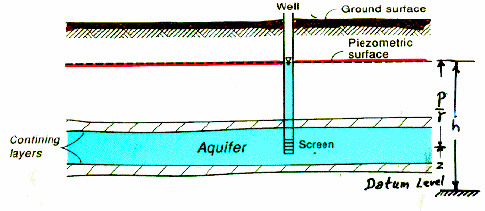
\includegraphics[width=0.99\linewidth]{conaq.jpg}

  Řez zvodní s volnou hladinou (výška zavodněné části je rovna rozdílu mezi piezometrickou výškou a dolní nepropustnou vrstvou).

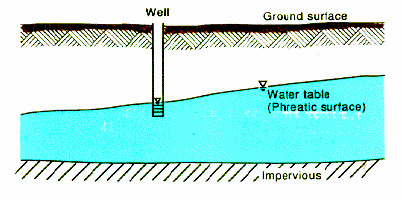
\includegraphics[width=0.99\linewidth]{phraq.jpg}
  
\end{minipage}


Zapište pomocí vhodných veličin, operátorů a rovnic následující vztahy, zákony nebo pozorování,
odpovězte na otázky a splňte úkoly.
\begin{enumerate}[A)]
\item \textit{Darcyho zákon vyjádřený pro celou zvodeň (od povrchu k nepropustnému podloží)}:
  Průtok na jednotku šířky, $\vec q$, má v izotropním prostředí směr
  maximálního poklesu piezometrické hladiny a co do velikosti je
  úměrný tomuto poklesu. Koeficient úměrnosti se nazývá koeficient
  průtočnosti nebo transmisivita a označuje se $T$.
\item Jak zpravidla modifikujeme předchozí odpověď, pokud zvodeň není
  izotropní a má v různých směrech různé vlastnosti?
\item Často pracujeme s veličinou \textit{filtrační rychlost} $\vec v_f$, která
  udává, jaký objem proteče jednotkovou plochou kolmo na směr proudění
  za jednotku času. Jaký bude vztah mezi $\vec v_f$ a $\vec q$? Uvažujte pouze
  speciální případ, kdy je $\vec v_f$ konstantní v celé tloušťce zvodnělé
  vrstvy $b$. (Tloušťka zvodnělé vrstvy $b$ je u proudění s volnou hladinou rovna vzdálenosti piezometrické hladiny od dolní nepropustné vrstvy a u proudění mezi nepropustnými vrstvami rovna vzdálenosti těchto vrstev.) 
  \stranka
\item \textit{Zákon zachování pro vodu}: Množství vody v daném místě (v metrech krychlových vody na metr čtvereční povrchu zvodně) označte $v$. Rychlost s jakou se kumuluje voda v daném místě v kubických
  metrech (vody) na čtvereční metr (povrchu zvodně) za den, tj. derivace $v$ podle času, je
  součtem
  \begin{itemize}\itemsep 0 pt
  \item vydatnosti zdrojů v tomto místě ($\sigma$, v kubických
    metrech vody na metr čtvereční povrchu zvodně za den, může se jednat například o zasakování srážek) a
  \item rychlosti, s jakou v daném místě klesá tok $\vec q$.
\end{itemize}
  Vyjádřete tento zákon kvantitativně pomocí vhodné rovnice.
\item Objem vody v podzemí souvisí s hladinou podzemní
  vody. \textit{Zásobnost} $S_s$ udává, jaký objem vody se uvolní na
  metru čtverečním povrchu zvodně, pokud se piezometrická hladina
  v tomto místě sníží o jednotku. U zvodně s volnou hladinou je tato
  veličina dána zejména pórovitostí půdy nebo horniny, u zvodně s
  napjatou hladinou souvisí se stlačitelností a proto je v tomto
  případě zásobnost velmi malá. Jaká je jednotka takto definované
  zásobnosti a jak souvisí rychlost s jakou roste objem vody v daném
  místě zvodně s rychlostí, s jakou roste piezometrická hladina
  v tomto místě?
\item Předchozí odpovědi spojte do rovnice 
  podzemní vody v anizotropním prostředí.
\end{enumerate}

\textit{Podle Jacob Bear, Modeling Groundwater Flow and Pollution a Charles Fitts, Groundwater Science.}

\reseni

\begin{enumerate}[A)]
\item $\vec q=-T \nabla h$ kde $T$ je koeficient průtočnosti a $-\nabla h$
  je vektor mířící ve směru nejrychlejšího poklesu piezometrické
  hladiny $h$ a vyjadřující rychlost tohoto poklesu.
\item $T$ je  $2\times 2$ matice
\item $\vec q=b\vec v_f$
\item $\frac{\partial v}{\partial t}=\sigma-\mathop{\mathrm{div}}\vec q$
\item Zásobnost je vlastně změna objemu (vody) na jednotkovou plochu
  (zvodně) vyvolaná  jednotkovou změnou délky (změna piezometrické hladiny),
  tj. derivace $v$ podle $h$ a jednotkově vychází bez rozměru. Platí tedy
  \begin{equation*}
    \derivace vh=S_s \end{equation*}
  kde $v$ je objem vody na
  metr čtvereční povrchu zvodně v daném místě. Po vynásobení rychlostí s jakou se
  mění piezometrická výška dostáváme
  \begin{equation*}
    \derivace vh \derivace ht=S_s\derivace ht
  \end{equation*}
   a po využití derivace složené funkce
  \begin{equation*}
    \derivace vt=S_s\derivace ht.
  \end{equation*}
  Toto se děje v libovolném místě zvodně. Protože $v$ a $h$ jsou i funkcemi proměnných $x$ a $y$ a protože souřadnice $x$ a $y$ jsou nezávislé na čase, stačí pro korektní zápis použít parciální derivace namísto obyčejné derivace, tj.
  \begin{equation*}
       \frac{\partial v}{\partial t} = S_s \frac {\partial h}{\partial t}.
     \end{equation*}
\item
  \begin{equation*}
    S_s\frac{\partial h}{\partial t}=\sigma - \mathop{\mathrm{div}} \left(-T\nabla h\right)
  \end{equation*}
  tj. 
  \begin{equation*}
    S_s\frac{\partial h}{\partial t}=\sigma + \mathop{\mathrm{div}} \left(T\nabla h\right)
  \end{equation*}

\end{enumerate}
\konec
\stranka

\subsection{Rovinné proudění podzemní vody podruhé}

Prozkoumáme podruhé rovinné proudění, kterému jsme se věnovali v
příkladě \ref{pokles}.

\begin{enumerate}[A)]
\item Rovnici podzemní vody ve 2D rozepište do složek. Uvažujte pro jednoduchost izotropní prostředí (transmisivita je skalární veličina, tj. ne matice a voda teče ve směru spádu piezometrické hladiny).
\item Napište rovnici z předchozího bodu pro \textit{stacionární} případ \textit{bez zdrojů} a pro případ, že funkce $h$ nezávisí na $y$. Uvažujte homogenní prostředí a zvodeň s volnou hladinou a vodorovnou dolní nepropustnou vrstvou, kde volíme nulovou hladinu $h$ (tj. transmisivita je tvaru $$T=kh,$$ kde $k$ je reálné číslo, ne funkce proměnných $x$ a $y$)
\item Ukážeme, že rovnice se dá vyřešit i bez znalosti řešení diferenciálních rovnic. Upravte vztah z předchozího bodu použitím zřejmé identity
  $(h^2)'=2 h h'$
  pro $h$ jako funkci proměnné  $x$, kde čárka značí derivaci podle $x$. Výsledkem bude podmínka, kterou musí splňovat funkce $h^2$ a odsud již najdete hledanou křivku snížení piezometrické hladiny. (Pokud je $h$ závislé jenom na $x$, plocha ohraničující zvodnělou vrstvu se z bočního pohledu promítne do křivky.)
\end{enumerate}


\reseni
\begin{enumerate}[A)]
\item $$S_s\frac{\partial h}{\partial t}=\sigma + \frac{\partial }{\partial x}\left (T \frac{\partial h}{\partial x} \right)
  +
  \frac{\partial }{\partial y}\left (T \frac{\partial h}{\partial y} \right)
  $$
\item Protože máme uvažovat stacionární případ, funkce $h$ nezávisí na $t$. Podle předpokladu $h$ nemá záviset ani na $y$. Proto platí $h=h(x)$, tj. derivace $h$ podle $t$ a podle $y$ jsou nulové.
  Protože nemáme uvažovat zdroje, je $\sigma$ také nulové. Protože máme uvažovat homogenní případ a $T=kh$, můžeme konstantu $k$ a dát před derivaci.  Rovnice má tvar
  $$0=k\frac{\partial }{\partial x}\left ( h\frac{\partial h}{\partial x} \right)
  $$
  anebo (využitím stručnějšího zápisu pro derivace funkce jedné proměnné)
  $$0=k(h h')'.$$
\item Dostáváme $h h' = \frac12 (h^2)'$ a po dosazení
$$0=k\left(\frac 12 (h^2)'\right )'.$$ Po vydělení rovnice konstantou $k$ a vynásobení faktorem $2$ dostaneme 
  $$0=(h^2)''.$$
  Druhá derivace funkce $h^2$ tedy musí být nula. Proto je $h^2$ nutně lineární funkcí proměnné $x$, tj. existují konstanty $C_1$ a $C_2$ tak, že platí $$h^2=C_1x+C_2.$$
  Křivka odpovídá výsledku příkladu  \ref{pokles}, kde je
  $$h^2=\frac{-2q}k x + \text{const.}$$
\end{enumerate}
\konec

\subsection{O Otesánkovi.}
Otesánek se vykrmil do tvaru koule o průměru $2{,}4\,\mathrm{m}$ a dále baští. Jeho objem roste konstantní rychlostí $0{,}002 \mathrm{m}^3/\mathrm{hod}$. Jak tato úloha souvisí s derivacemi a jak rychle roste průměr koule (Otesánka)? $$V=\frac 16 \pi d^3$$

\subsection{Dlouhý a Bystrozraký.} Dlouhý má na ramenou Bystrozrakého ve výšce $4$ metry. Bystrozraký hledá princeznu a vzdálenost, na kterou vidí, je dána vzorcem pro vzdálenost k horizontu, tj. $$H=k\sqrt {h},$$ kde $H$ je vzdálenost k horizontu v kilometrech, $h$ je výška pozorovatele nad povrchem  v metrech  a $k$ je konstanta.
  Dlouhý roste rychlostí $0{,}1\,\mathrm{m} \mathrm{s}^{-1}$.
Jak tato úloha souvisí s derivacemi a jak rychle roste vzdálenost na kterou Bystrozraký vidí?

\subsection{Nábytek bez atestu}

Formaldehyd se z dřevěného výrobku v malé nevětrané místnosti uvolňuje jenom do dosažení určité rovnovážné koncentrace. Rychlost, s jakou přibývá množství formaldehydu ve vzduchu v místnosti, je úměrná množství, která do této rovnovážné koncentrace chybí. Zapište tento proces pomocí vhodného matematického modelu (diferenciální rovnice).

\subsection{Kontaminovaný salát} Bakterie na kontaminovaném salátu se množí rychlostí  $$2e^{0.1t}\text{ milionů bakterií/den,}$$  kde $t$ je čas ve dnech. Pokud je to možné, určete, o~kolik se změní množství bakterií za čtyři dny. Pokud není dost informací, vysvětlete, jaké další informace potřebujeme.


\subsection{Nádrž na zavlažování}

Nádrž má tvar válce a je do poloviny naplněna vodou. Máme tři různé úlohy.
\begin{enumerate}[(A)]\itemsep 0 pt
\item Do nádrže teče voda konstantní rychlostí. Rychlost, s jakou roste hladina, je konstantní.
\item Dírou ve dně vytéká voda. Rychlost, s jakou klesá hladina, je úměrná odmocnině z výšky hladiny.
\item Z nádrže vytéká dírou ve dně voda (tj. stejná situace jako v předchozím modelu) a navíc konstantní rychlostí odebíráme vodu na zavlažování.
\end{enumerate}
Každý děj zapište pomocí
vhodného matematického modelu. Zajímá nás
hloubka vody v nádrži. Výška nádrže nás
nelimituje (nádrž v úloze A nepřeteče).


\subsection{Vlčí mák}
Vlčí mák je oblíbený letní plevel
  s obrovskou nadprodukcí
  semen. Předpokládejme, že rychlost
  s jakou roste populace vlčího máku je
  úměrná velikosti populace. Vyjádřete
  tento růst pomocí vhodné diferenciální
  rovnice.

  \subsection{Ošoupané medaile}

  Dana Zátopková vozila svoji zlatou medaili po besídkách a nechávala ji
    zde kolovat mezi diváky. Tím se medaile otírala a ztrácela hmotnost. Pokusíme
    se popsat tento děj. Předpokládejme, že s odstupem od olympiády intenzita
    besídek slábne a rychlost otírání se snižuje. Jaký bude úbytek zlata na
    medaili za první rok, pokud předpokládáme, že rychlost s jakou se mění
    hmotnost $m$ medaile je $\frac{\mathrm d m}{\mathrm dt}=-\frac{1}{t+1}$
    mikrogramů za týden?

    \subsection{Brýle}

    \begin{enumerate}
 \item Nechť $\varphi=f(a)$ je funkce, která
  udává jak závisí počet dioptrií $\varphi$ pro
  korekci krátkozrakosti na vzdálenosti $a$
  (v metrech), na kterou ještě oko vidí
  ostře. V jakých jednotkách bude
  vyjádřena derivace
  $\frac{\mathrm d\varphi}{\mathrm da}$ a jaká
  bude slovní interpretace této derivace?
\item Funkce z předchozího bodu je
  $\varphi=-\frac 1a$. Nechť $a=10\,\mathrm m$
  a nechť se $a$ zkracuje rychlostí $0.1$
  metru za rok. Napište, jak souvisí rychlost s jakou se mění $a$ s rychlostí, s jakou se mění $\varphi$ a pro daný případ určete, jak rychle se mění počet
  dioptrií nutných pro korekci této vady?

\end{enumerate}



\subsection{Rychlost zvuku ve dřevě}

Rychlost zvuku v pevné látce je dána vzorcem $c=\sqrt{\frac E\varrho}$ kde $c$ je rychlost zvuku v metrech za sekundu, $E$ Yougův modul pružnosti v pascalech a $\varrho$ hustota v kilogramech na metr krychlový. U dřeva předpokládejme, že v závislosti na vlhkosti se $\varrho$ může měnit a $E$ je konstantní. Určete derivaci $\frac{\mathrm dc}{\mathrm d\varrho}$. Pokud například pro břízu $\rho = 640 \,\mathrm{kg}\,\mathrm{m}^{-3}$ je tato derivace číselně rovna hodnotě $-3.3$, doplňte jednotku a napište slovní interpretaci této derivace.

\subsection{Růst ryb}

Na rozdíl od jiných živočichů jsou malé ryby jsou přibližně zmenšeniny
    velkých ryb a proto je u nich hmotnost přibližně úměrná třetí mocnině
    délky. Najděte souvislost mezi rychlostí s jakou roste hmotnost kapra a
    rychlostí, s jakou roste délka kapra.



\subsection{Termohrnek z rozemleté televize}    
Termohrnek bez atestu, vyrobený z rozemletého plastu ze staré
elektroniky, uvolňuje do nápoje zdravotně závadné materiály.
Například zpomalovače hoření, BFR. Předpokládejme, že tempo se kterým
se BFR vylučuje do nápoje se snižuje s rostoucí kontaminací nápoje a s
klesající teplotou nápoje, tj. klesá v čase. Vhodným modelem může být
například
    $$r(t)=(10-2t) \,\mathrm{\mu g}/\mathrm{hod},$$ kde $r(t)$ je rychlost vylučování
    BFR do nápoje v čase $t$ v mikrogramech za hodinu a $t$ je čas v hodinách. Vypočtěte, jaké množství
    BFR se do nápoje uvolní za první hodinu a porovnejte s
    hodnotou, která se uvolní za druhou hodinu.


    \subsection{Padání sněhu s proměnnou intenzitou}

    O půlnoci začal padat sníh rychlostí $6$ centimetrů za hodinu. Intenzita
    slábla a v poledne přestalo sněžit. V tomto období je možné modelovat
    rychlost padání sněhu funkcí $r(t)$, která splňuje $r(0)=6$ a
    $r(12)=0$, kde $t$ je počet hodin od půlnoci v
    hodinách a $r$ je rychlost v centimetrech za hodinu. Kolik sněhu napadalo? Zapište obecně a poté pro nejjednodušší funkci, která splňuje uvedené požadavky, pro funkci $$r(t)=6-\frac 12 t.$$
    (Slunce nesvítilo a bylo pořád pod nulou.)


    \subsection{Vyzařování tepla}

    \begin{enumerate}
    \item Vyzařování ve wattech na metr čtvereční je dáno Stefanovým-Bolzmanovým zákonem
      $$Q=\sigma T^4,$$
      kde $T$ je teplota (v Kelvinech), $\sigma$ konstanta a $Q$ vyzářený výkon ve wattech na metr čtvereční. Vypočtěte derivaci
      $$\frac{\mathrm dQ}{\mathrm dT}.$$
    \item Derivace z předchozího bodu pro $T=300K$ je číselně rovna $6.12$. Doplňte jednotku a napište slovní interpretaci této derivace.
    \end{enumerate}
    Poznámka: Termodynamická teplota v Kelvinech je teplota ve stupních Celsia zmenšená o hodnotu 273.15.


\subsection{Odvození rovnice vedení tepla v 1D}

Pokračujeme v úloze s vedením tepla v 1D. S využitím výsledků této úlohy zapište kvantitativně následující zákony.
\begin{enumerate}[a)]
\item Tok tepla (směrem doprava) je úměrný rychlosti, s jakou klesá
teplota (směrem doprava).
\item Rychlost, s jakou v daném bodě ubývá tok tepla jako funkce polohy je úměrná rychlosti, s jakou roste teplota v daném bodě, jako funkce času, tj. teplo které ``ztratíme'' na toku tepla se projeví odpovídajícím zvýšením teploty. 
\end{enumerate}

Poté oba zákony spojte do jednoho vztahu a odvodíte rovnici vedení tepla v 1D.
Ukažte, že pokud bude tyč homogenní, po nastolení rovnováhy bude teplota lineární funkcí polohy.

\reseni

\begin{enumerate}[a)]
\item To, že tok tepla (směrem doprava) je úměrný rychlosti, s jakou klesá
  teplota (směrem doprava) vyjádříme rovnicí
  \begin{equation*}
    q=-k_1\frac {\partial T}{\partial x}
  \end{equation*}
  kde $k_1$ je konstanta úměrnosti a $-\frac {\partial T}{\partial x}$ udává, jak klesá teplota směrem doprava.
\item To, že rychlost, s jakou v daném bodě ubývá tok tepla jako funkce polohy je úměrná rychlosti, s jakou roste teplota v daném bodě, jako funkce času, tj. teplo které ``ztratíme'' na toku tepla se projeví zvýšením teploty, vyjádříme rovnicí
  \begin{equation*}
-\frac{\partial q}{\partial x} = k_2    \frac{\partial T}{\partial t},
  \end{equation*}
  kde $k_2$ je konstanta úměrnosti a $\frac {\partial T}{\partial t}$ udává, jak roste teplota jako funkce času.    
\end{enumerate}
Spojením dostaneme
  \begin{equation*}
-\frac{\partial }{\partial x}
\left( -k_1\frac {\partial T}{\partial x} \right)  = k_2 \frac{\partial T}{\partial t}  ,
  \end{equation*}
  a po úpravě
  \begin{equation*}
  k_2  \frac{\partial T}{\partial t} = \frac{\partial }{\partial x}
\left( k_1\frac {\partial T}{\partial x} \right).    
\end{equation*}
Častěji se tato rovnice píše ve tvaru 
  \begin{equation*}
\rho c  \frac{\partial T}{\partial t} = \frac{\partial }{\partial x}
\left( k_1\frac {\partial T}{\partial x} \right),    
\end{equation*}
protože konstantu ${k_2}$ můžeme vyjádřit pomocí fyzikálních charakteristik hustota $\rho$ a měrná tepelná kapacita $c$.

V rovnovážném stavu je derivace podle času nulová a dostáváme
  \begin{equation*}
\frac{\partial }{\partial x}
\left( k_1\frac {\partial T}{\partial x} \right)=0
\end{equation*}
a pro homogenní tyč je $k_1$ konstanta a proto 
  \begin{equation*}
k_1 \frac{\partial }{\partial x}
\left( \frac {\partial T}{\partial x} \right)=0.
\end{equation*}
Druhá derivace podle $x$ je tedy nulová, což znamená, že $T$  je vzhledem k $x$ lineární.

\konec

\obrazek{destnik}[-20pt]

\subsection{Kapka vody I}
Předpokládejme, že kapka vody má kulovitý tvar a při dešti roste tak, že objem
jako funkce času se zvětšuje rychlostí úměrnou povrchu. (Kondenzace vodních par probíhá
na povrchu a výsledek této kondenzace, voda, zvětšuje objem.) Přepište tento scénář do matematického modelu a všechny závislé proměnné vyjádřete pomocí objemu.

\textit{Klasický případ, kdy v zadání figuruje rychlost s jakou se mění objem, tj. derivace objemu, a tento vztah zformulujeme matematicky. Protože tato formulace obsahuje povrch koule, je nutné tento povrch přepočítat na objem.}

\reseni Je-li $V$ objem a $S$ povrch koule, je $\derivace Vt$ rychlost s jakou roste objem koule a přepisem zadání do kvantitativních vztahů dostáváme
$$\frac {\mathrm dV}{\mathrm dt}= k_1S, $$ kde $k$ je konstanta úměrnosti. Protože díky podobnosti pro kouli platí $S=k_2 V^{2/3}$ kde $k_2$ je vhodná konstanta, dostáváme 
$$\frac{\mathrm dV}{\mathrm dt}=k_1k_2 V^{2/3}.$$ Spojením obou konstant do jediné $k=k_1k_2$ obdržíme výsledný model 
$$\frac{\mathrm dV}{\mathrm dt}=kV^{2/3}.$$ 
\konec



\obrazek{destnik}[-20pt]

\subsection{Kapka vody II}
Předpokládejme jako v předchozím příkladě, že kapka vody má kulovitý tvar a při dešti roste tak, že objem
jako funkce času se zvětšuje rychlostí úměrnou povrchu. Ukažte,
že poloměr jako funkce času roste konstantní rychlostí.

\textit{Klasický případ, kdy v zadání figuruje rychlost s jakou se mění objem, tj. derivace objemu, ale protože nás zajímá jiná veličina, musíme ještě najít vztah mezi rychlostí, s jakou roste objem, a rychlostí, s jakou roste poloměr.}

\reseni Je-li $V=\frac 43 \pi r^3$ objem kulovité kapky, platí
(derivováním) $$\frac {\mathrm dV}{\mathrm dt}=4\pi r^2\frac{\mathrm dr}{\mathrm dt}$$
a (přepisem zadání do řeči derivací a s využitím vzorce pro povrch koule)
$$\frac {\mathrm dV}{\mathrm dt}= k 4\pi r^2, $$ kde $k$ je konstanta úměrnosti. Odsud
$$4\pi r^2\frac{\mathrm dr}{\mathrm dt}=k 4\pi r^2$$
a
$$\frac{\mathrm dr}{\mathrm dt}=k.$$ Napravo je konstanta, poloměr tedy roste konstantní rychlostí.
\konec


\stranka

\subsection{Výpočet $\pi$}  Pro $n\neq -1$ vypočtěte integrály
$$\int_0^1 x^n\,\mathrm dx \qquad \text{a} \qquad \int_0^1
\frac{1}{1+x^2}\,\mathrm dx.$$

\textbf{Poznámka:} Vzorec pro součet geometrické
řady s kvocientem $-x^2$ je $$\frac{1}{1+x^2}=1-x^2+x^4-x^6+\cdots$$ po integrování (a po
zapojení teorie nekonečných řad, která ospravedlní integrování člen po
členu a to, že v horní mezi je $x=1$, přestože řada pro $x=1$ nekonverguje) dává
$$
\int_0^1 \frac{1}{1+x^2}\,\mathrm dx
=
\int_0^1 1\,\mathrm dx
-
\int_0^1 x^2\,\mathrm dx
+
\int_0^1 x^4\,\mathrm dx
-
\int_0^1 x^6\,\mathrm dx
+\cdots .
$$
Po zintegrování vlevo dostaneme veličinu obsahující $\pi$ a vpravo
součet racionálních čísel. Tím je možné odhadnout hodnotu $\pi$. Tato
technika, používaná v~jistých obměnách v~17. a 18. století, je mnohem
efektivnější pro výpočet $\pi$, než starší metoda pravidelných
mnohoúhelníků vepsaných do kružnice. Dnes máme k dispozici řady,
které k hodnotě $\pi$ konvergují mnohem rychleji.

\reseni

Platí $$\int_0^1 \frac {1}{x^2+1}\,\mathrm dx=\left [\arctg x\right]_0^1=\arctg 1 - \arctg 0 = \frac \pi 4$$
a
$$\int_0^1 x^n \,\mathrm dx=\left[\frac 1{n+1} x^{n+1}\right]_0^1=\frac 1{n+1}.$$
Proto integrováním vztahu
$$\frac{1}{1+x^2}=1-x^2+x^4-x^6+\cdots$$
dostaneme
$$\frac{\pi}{4}=1-\frac 13 +\frac 15 - \frac 17+\cdots$$
a vyjádření $\pi$ pomocí řady je
$$\pi=4-\frac 43 +\frac 45 - \frac 47+\cdots .$$
Čím více členů započítáme, tím je aproximace čísla $\pi$ přesnější.
\konec



\obrazek{pneumatika.jpg}

\subsection{Tlak v pneumatice}

Tlakem v pneumatice rozumíme ve skutečnosti přetlak vůči atmosférickému tlaku. Poškozená pneumatika ztrácí vzduch tak, že množství vzduchu v pneumatice klesá rychlostí, která je úměrná tomuto tlaku. Tlak v~pneumatice a množství vzduchu v pneumatice jsou také navzájem úměrné. Napište matematický model popisující pokles tlaku v čase.


\reseni

Je-li $m$ hmotnost vzduchu v pneumatice a $p$ tlak, z úměrnosti mezi oběma veličinami plyne $$\frac{\mathrm dm}{\mathrm dt}=k_1\frac{\mathrm dp}{\mathrm dt}.$$
Podle zadání platí
$$\frac{\mathrm dm}{\mathrm dt}=-k_2p.$$
Odsud $$\frac{\mathrm dp}{\mathrm dt}=-kp,$$
kde $k$ je konstanta, která vznikne sloučením konstant $k_1$ a $k_2$.

\konec

\subsection{Kvadratický moment kruhu}

\subsection{Stacionární vedení tepla ve válcovém prostředí}


\subsection{Chemická reakce}
Při chemické reakci se spotřebovává enzym tak, že spolu za přítomnosti
katalyzátoru reagují dvě molekuly tohoto enzymu. V důsledku toho
rychlost s jakou se snižuje množství enzymu je úměrná druhé mocnině
koncentrace a tedy i druhé mocnině množství tohoto enyzmu. Napište
diferenciální rovnici popisující tento děj.

\subsection{Ondatra} V roce 1905 vysadil na svém panství
  hrabě Colloredo-Mansfeld několik párů
  ondatry, které dovezl z
  Ameriky. Ondatra se díky absenci
  přirozených nepřátel rychle rozšířila
  po celé Evropě. Předpokládejme, že
  oblast zasažená rozšířením ondatry má
  tvar kruhu o poloměru $230\, \mathrm{km}$ a tento
  poloměr roste rychlostí
  $30 \,\mathrm{km}/\mathrm{rok}$. Jak
  rychle roste plocha kruhu? Jak rychle
  roste obvod kruhu?


\subsection{Akumulátor} Teplota studeného akumulátoru přeneseného do místnosti o pokojové teplotě roste rychlostí 
  \begin{equation*}
     \frac 12e^{-t}\  {}^\circ\mathrm{C}/\mathrm{hod}
  \end{equation*}
  kde $t$ je čas v
  hodinách. Najděte změnu teploty akumulátoru za prvních pět hodin.

\subsection{Kmen stromu}
  Kmen můžeme v určitých
částech stromu primitivně modelovat
válcem. Uvažujme délkový metr kmene,
tj. válec o výšce 1m a poloměru
$r$. Hmotnost válce je
\begin{equation*}
m=V\rho =\pi \rho
r^2,
\end{equation*}
kde $\rho=700 \mathrm{kg/m^3}$ je hustota
dřeva. Poloměr kmene roste rychlostí
$0{,}01\,\mathrm{m/rok}$. Najděte vztah
mezi rychlostí růstu poloměru válce a
rychlostí růstu hmotnosti válce. Určete
rychlost s jakou roste hmotnost
v~okamžiku, kdy poloměr kmene je
$r=0{,}20\,\mathrm{m}$.
